\RequirePackage[l2tabu,orthodox]{nag}

% The one-sided layout is retained for the submitted draft.
%\documentclass[headsepline,footsepline,footinclude=false,fontsize=11pt,paper=a4,listof=totoc,bibliography=totoc,BCOR=12mm,DIV=12]{scrbook} % two-sided % original source stated: BCOR=12mm,DIV=12
\documentclass[headsepline,footsepline,footinclude=false,oneside,fontsize=11pt,paper=a4,listof=totoc,bibliography=totoc,DIV=12]{scrbook} % one-sided

% Bibliography and citation styling are defined centrally in settings.tex.
\PassOptionsToPackage{table,svgnames,dvipsnames}{xcolor}

\usepackage[utf8]{inputenc}
\usepackage[T1]{fontenc}
\usepackage[sc]{mathpazo}
\usepackage[ngerman,english]{babel} % english is the same as american or USenglish
\usepackage[autostyle]{csquotes}
\usepackage[%
  backend=biber,
  url=true,
  style=numeric, % alphabetic, numeric
  sorting=none, % default == nty, https://tex.stackexchange.com/questions/51434/biblatex-citation-order
  maxnames=4,
  minnames=3,
  maxbibnames=99,
  giveninits,
  uniquename=init]{biblatex} % numeric citations in order of first appearance
\usepackage{graphicx}
\usepackage{scrhack} % necessary for listings package
\usepackage{listings}
\usepackage{lstautogobble}
\usepackage{tikz}
\usepackage{pgfplots}
\usepackage{pgfplotstable}
\usepackage{booktabs} % for better looking table creations, but bad with vertical lines by design (package creator despises vertical lines)
\usepackage[final]{microtype}
\usepackage{caption}
% Keep figures and tables inside the section/subsection that introduces them.
% Full-page figures may float within that unit, but must precede its next heading.
\usepackage[section]{placeins}
\usepackage{etoolbox}
\AtBeginDocument{%
  \pretocmd{\subsection}{\FloatBarrier}{}%
    {\PackageError{thesis}{Cannot add subsection float barrier}{}}%
  \pretocmd{\subsubsection}{\FloatBarrier}{}%
    {\PackageError{thesis}{Cannot add subsubsection float barrier}{}}%
}
\usepackage[hidelinks]{hyperref} % hidelinks removes colored boxes around references and links
\usepackage{ifthen} % for comparison of the current language and changing of the thesis layout
\usepackage{pdftexcmds} % string compare to work with all engines
\usepackage{paralist} % for condensed enumerations or lists
\usepackage{subfig} % for having figures side by side
\usepackage{siunitx} % for physical accurate units and other numerical presentations
\usepackage{multirow} % makes it possible to have bigger cells over multiple rows in a table
\usepackage{array} % different options for table cell orientation
\usepackage{makecell} % allows nice manual configuration of cells with linebreaks in \thead and \makecell with alignments
\usepackage{pdfpages} % for including multiple pages of pdfs
\usepackage{adjustbox} % can center content wider than the \textwidth
\usepackage{tablefootnote} % for footnotes in tables as \tablefootnote
\usepackage{threeparttable} % another way to add footnotes as \tablenotes with \item [x] <your footnote> after setting \tnote{x} 


% https://tex.stackexchange.com/questions/42619/x-mark-to-match-checkmark
\usepackage{amssymb}% http://ctan.org/pkg/amssymb
\usepackage{pifont}% http://ctan.org/pkg/pifont
\newcommand{\cmark}{\ding{51}}%
\newcommand{\xmark}{\ding{55}}%


\usepackage[acronym,xindy,toc]{glossaries} % separate acronym and glossary lists
\makeglossaries
\loadglsentries{pages/glossary.tex} % important update for glossaries, before document


\bibliography{bibliography}
\AtBeginBibliography{\sloppy}

\setkomafont{disposition}{\normalfont\bfseries} % use serif font for headings
\linespread{1.05} % adjust line spread for mathpazo font

% Add table of contents to PDF bookmarks
\BeforeTOCHead[toc]{{\cleardoublepage\pdfbookmark[0]{\contentsname}{toc}}}

% Define TUM corporate design colors
% Taken from http://portal.mytum.de/corporatedesign/index_print/vorlagen/index_farben
\definecolor{TUMBlue}{HTML}{0065BD}
\definecolor{TUMSecondaryBlue}{HTML}{005293}
\definecolor{TUMSecondaryBlue2}{HTML}{003359}
\definecolor{TUMBlack}{HTML}{000000}
\definecolor{TUMWhite}{HTML}{FFFFFF}
\definecolor{TUMDarkGray}{HTML}{333333}
\definecolor{TUMGray}{HTML}{808080}
\definecolor{TUMLightGray}{HTML}{CCCCC6}
\definecolor{TUMAccentGray}{HTML}{DAD7CB}
\definecolor{TUMAccentOrange}{HTML}{E37222}
\definecolor{TUMAccentGreen}{HTML}{A2AD00}
\definecolor{TUMAccentLightBlue}{HTML}{98C6EA}
\definecolor{TUMAccentBlue}{HTML}{64A0C8}

% Settings for pgfplots
\pgfplotsset{compat=newest}
\pgfplotsset{
  % For available color names, see http://www.latextemplates.com/svgnames-colors
  cycle list={TUMBlue\\TUMAccentOrange\\TUMAccentGreen\\TUMSecondaryBlue2\\TUMDarkGray\\},
}

% Settings for lstlistings

% Use this for basic highlighting
\lstset{%
  basicstyle=\ttfamily,
  columns=fullflexible,
  autogobble,
  keywordstyle=\bfseries\color{TUMBlue},
  stringstyle=\color{TUMAccentGreen}
}

% use this for C# highlighting
% %\setmonofont{Consolas} %to be used with XeLaTeX or LuaLaTeX
% \definecolor{bluekeywords}{rgb}{0,0,1}
% \definecolor{greencomments}{rgb}{0,0.5,0}
% \definecolor{redstrings}{rgb}{0.64,0.08,0.08}
% \definecolor{xmlcomments}{rgb}{0.5,0.5,0.5}
% \definecolor{types}{rgb}{0.17,0.57,0.68}

% \lstset{language=[Sharp]C,
% captionpos=b,
% %numbers=left, % numbering
% %numberstyle=\tiny, % small row numbers
% frame=lines, % above and underneath of listings is a line
% showspaces=false,
% showtabs=false,
% breaklines=true,
% showstringspaces=false,
% breakatwhitespace=true,
% escapeinside={(*@}{@*)},
% commentstyle=\color{greencomments},
% morekeywords={partial, var, value, get, set},
% keywordstyle=\color{bluekeywords},
% stringstyle=\color{redstrings},
% basicstyle=\ttfamily\small,
% }

% Settings for search order of pictures
\graphicspath{
    {logos/}
    {figures/}
}

% Set up hyphenation rules for the language package when mistakes happen
\babelhyphenation[english]{
an-oth-er
ex-am-ple
}

% Decide between
%\newcommand{\todo}[1]{\textbf{\textsc{\textcolor{TUMAccentOrange}{(TODO: #1)}}}} % for one paragraph, otherwise error!
%\newcommand{\done}[1]{\textit{\textsc{\textcolor{TUMAccentBlue}{(Done: #1)}}}} % for one paragraph, otherwise error!
% and
\newcommand{\todo}[1]{{\bfseries{\scshape{\color{TUMAccentOrange}[(TODO: #1)]}}}} % for multiple paragraphs
\newcommand{\done}[1]{{\itshape{\scshape{\color{TUMAccentBlue}[(Done: #1)]}}}} % for multiple paragraphs
% for error handling of intended behavior in your latex documents.

\newcommand{\tabitem}{~~\llap{\textbullet}~~}

\newcolumntype{P}[1]{>{\centering\arraybackslash}p{#1}} % for horizontal alignment with limited column width
\newcolumntype{M}[1]{>{\centering\arraybackslash}m{#1}} % for horizontal and vertical alignment with limited column width
\newcolumntype{L}[1]{>{\raggedright\arraybackslash}m{#1}} % for vertical alignment left with limited column width
\newcolumntype{R}[1]{>{\raggedleft\arraybackslash}m{#1}} % for vertical alignment right with limited column width


\newcommand*{\getUniversity}{Technische Universität München}
\newcommand*{\getFaculty}{Department of Informatics}
\newcommand*{\getTitle}{On the Feasibility of Pixel-Free Visual Odometry Using Video Codec Motion Vectors}
\newcommand*{\getTitleGer}{Zur Machbarkeit pixelfreier visueller Odometrie mit Bewegungsvektoren aus Videocodecs}
\newcommand*{\getAuthor}{Emir Özer}
\newcommand*{\getDoctype}{Master's Thesis in Informatics}
\newcommand*{\getSupervisor}{Mateo de Mayo}
\newcommand*{\getExaminer}{Daniel Cremers}
\newcommand*{\getSubmissionDate}{23 September 2026}
\newcommand*{\getSubmissionLocation}{Munich}

\hypersetup{pdftitle={\getTitle},pdfauthor={\getAuthor}}

\begin{document}

% English is the main thesis language.
%\selectlanguage{ngerman}
\selectlanguage{english}

% Set page numbering to avoid "destination with the same identifier has been already used" warning for cover page.
% (see https://en.wikibooks.org/wiki/LaTeX/Hyperlinks#Problems_with_Links_and_Pages).
\pagenumbering{alph}
\begin{titlepage}
  % HACK for two-sided documents: ignore binding correction for cover page.
  % Adapted from Markus Kohm's KOMA-Script titlepage=firstiscover handling.
  % See http://mirrors.ctan.org/macros/latex/contrib/koma-script/scrkernel-title.dtx,
  % \maketitle macro.
  \oddsidemargin=\evensidemargin\relax
  \textwidth=\dimexpr\paperwidth-2\evensidemargin-2in\relax
  \hsize=\textwidth\relax

  \centering

  \IfFileExists{logos/tum.pdf}{%
    
\includegraphics[height=20mm]{logos/tum.pdf}
  }{%
    \vspace*{20mm}
  }

  \vspace{5mm}
  {\huge\MakeUppercase{\getFaculty{}}}\\

  \vspace{5mm}
  {\large\MakeUppercase{\getUniversity{}}}\\

  \vspace{20mm}
  {\Large \getDoctype{}}

  \vspace{15mm}
  \makeatletter
  \ifthenelse{\pdf@strcmp{\languagename}{english}=0}
  {\huge\bfseries \getTitle{}}
  {\huge\bfseries \getTitleGer{}}
  \makeatother

  \vspace{15mm}
  {\LARGE \getAuthor{}}

  \IfFileExists{logos/faculty.png}{%
    \vfill{}
    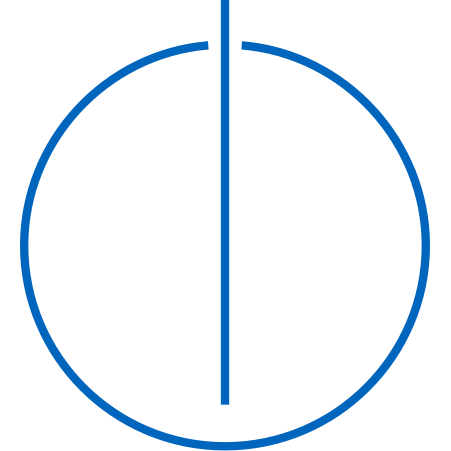
\includegraphics[height=20mm]{logos/faculty.png}
  }{}
\end{titlepage}


\frontmatter{}

\begin{titlepage}
  \centering

  \IfFileExists{logos/tum.pdf}{%
    
\includegraphics[height=20mm]{logos/tum.pdf}
  }{%
    \vspace*{20mm}
  }

  \vspace{5mm}
  {\huge\MakeUppercase{\getFaculty{}}}\\

  \vspace{5mm}
  {\large\MakeUppercase{\getUniversity{}}}\\

  \vspace{20mm}
  {\Large \getDoctype{}}

  \makeatletter
  \vspace{15mm}
  \ifthenelse{\pdf@strcmp{\languagename}{english}=0}
  {
  {\huge\bfseries \getTitle{}}

  \vspace{10mm}
  {\huge\bfseries \foreignlanguage{ngerman}{\getTitleGer{}}}
  }
  {
  {\huge\bfseries \getTitleGer{}}

  \vspace{10mm}
  {\huge\bfseries \foreignlanguage{english}{\getTitle{}}}
  }
  \makeatother

  \vspace{15mm}
  \begin{tabular}{l l}
    Author:          & \getAuthor{} \\
    Supervisor:      & \getSupervisor{} \\
    Examiner:        & \getExaminer{} \\
    Submission Date: & \getSubmissionDate{} \\
  \end{tabular}

  \IfFileExists{logos/faculty.png}{%
    \vfill{}
    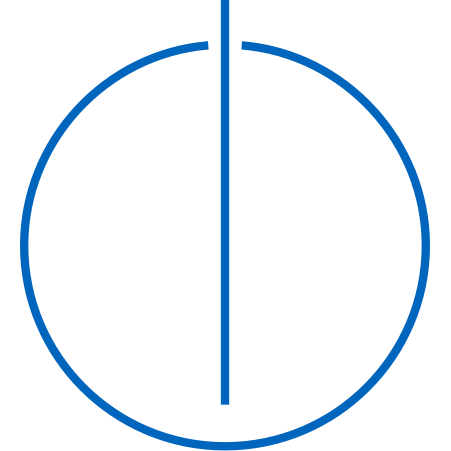
\includegraphics[height=20mm]{logos/faculty.png}
  }{}
\end{titlepage}

\cleardoublepage{}

\thispagestyle{empty}
\vspace*{0.8\textheight}
\noindent
\makeatletter
\ifthenelse{\pdf@strcmp{\languagename}{english}=0}
{I confirm that this \MakeLowercase{\getDoctype{}} is my own work and I have documented all sources and material used.}
{Ich versichere, dass ich diese \getDoctype{} selbstständig verfasst und nur die angegebenen Quellen und Hilfsmittel verwendet habe.}
\makeatother

\vspace{15mm}
\noindent
\getSubmissionLocation{}, \getSubmissionDate{} \hspace{50mm} \getAuthor{}

\cleardoublepage{}

\makeatletter
\ifthenelse{\pdf@strcmp{\languagename}{english}=0}
{\addcontentsline{toc}{chapter}{Acknowledgments}}
{\addcontentsline{toc}{chapter}{Danksagungen}}
\makeatother
\thispagestyle{empty}

\vspace*{20mm}

\begin{center}
\makeatletter
\ifthenelse{\pdf@strcmp{\languagename}{english}=0}
{\usekomafont{section} Acknowledgments}
{\usekomafont{section} Danksagungen}
\makeatother
\end{center}

\vspace{10mm}

I thank my supervisor and examiner for their guidance and feedback throughout
this project. I am also grateful to the colleagues, friends, and family members
who supported the work and the preparation of this thesis.

\cleardoublepage{}

\chapter{\abstractname}

Wearables and small drones need to understand how they move while operating
with limited power and computation. Visual odometry estimates this movement
from camera images, usually by tracking image features over time. Yet many
camera devices already contain dedicated hardware that searches for matching
image regions to compress video. Could the motion information produced by
this widely available hardware also support camera tracking?

This thesis explores that possibility using motion vectors from H.264 video
compression. These vectors describe how the encoder predicts image blocks;
they are designed to save data, so they do not necessarily follow the same
physical points over time. The proposed method combines vectors from two
cameras with known camera geometry to estimate depth and camera movement.
Its tracking and motion estimation use these measurements without consulting
image pixels. This approach is compatible with compress-then-analyze: a
camera could send the required compressed streams to a companion phone,
which reuses their motion information for localisation.

Experiments on an established drone benchmark recover coherent camera
trajectories, particularly on easier sequences. More demanding sequences
expose limitations, and methods that refine their tracks using image pixels
remain more accurate overall. The results nevertheless demonstrate that
useful camera tracking from codec motion vectors is feasible. They provide
one starting point for turning existing video-processing resources into a
source of geometric information. The experiments establish this possibility;
live hardware operation and the potential energy savings remain to be
evaluated.


\makeatletter
\ifthenelse{\pdf@strcmp{\languagename}{english}=0}
{\renewcommand{\abstractname}{Kurzfassung}}
{\renewcommand{\abstractname}{Abstract}}
\makeatother

\chapter{\abstractname}

\begin{otherlanguage}{ngerman}
\sisetup{locale=DE}

Wearables und kleine Drohnen müssen ihre eigene Bewegung erfassen können,
obwohl ihnen nur begrenzte Energie und Rechenleistung zur Verfügung stehen.
Visuelle Odometrie schätzt diese Bewegung aus Kamerabildern, üblicherweise
durch die Verfolgung von Bildmerkmalen über die Zeit. Viele Kamerageräte
enthalten jedoch bereits spezialisierte Hardware, die zur Videokompression
nach übereinstimmenden Bildregionen sucht. Könnten die dabei gewonnenen
Bewegungsinformationen auch zur Schätzung der Kamerabewegung dienen?

Diese Arbeit untersucht diese Möglichkeit anhand von Bewegungsvektoren
aus der H.264-Videokompression. Die Vektoren beschreiben, wie der Encoder
Bildblöcke vorhersagt. Da sie der Datenreduktion dienen, verfolgen sie nicht
zwangsläufig dieselben physischen Punkte über die Zeit. Das vorgeschlagene
Verfahren kombiniert Vektoren aus zwei Kameras mit bekannter Kamerageometrie,
um Tiefe und Kamerabewegung zu schätzen. Die Verfolgung und Bewegungsschätzung
nutzen diese Messungen, ohne auf Bildpixel zuzugreifen. Dieser Ansatz ist
mit Compress-then-Analyze vereinbar: Eine Kamera könnte die benötigten
komprimierten Videoströme an ein gekoppeltes Smartphone senden, das deren
Bewegungsinformationen für die Lokalisierung wiederverwendet.

Experimente auf einem etablierten Drohnen-Benchmark liefern schlüssige
Kameratrajektorien, insbesondere auf einfacheren Sequenzen. Anspruchsvollere
Sequenzen zeigen Grenzen auf; Verfahren, die ihre Korrespondenzen anhand von
Bildpixeln verfeinern, bleiben insgesamt genauer. Dennoch belegen die
Ergebnisse, dass eine brauchbare Schätzung der Kamerabewegung allein aus
Codec-Bewegungsvektoren möglich ist. Sie bieten einen Ausgangspunkt dafür,
vorhandene Ressourcen zur Videoverarbeitung als Quelle geometrischer
Informationen zu nutzen. Die Experimente zeigen diese Machbarkeit; der
Live-Betrieb auf entsprechender Hardware und mögliche Energieeinsparungen
müssen noch untersucht werden.

\end{otherlanguage}


% Undo the name switch
\makeatletter
\ifthenelse{\pdf@strcmp{\languagename}{english}=0}
{\renewcommand{\abstractname}{Abstract}}
{\renewcommand{\abstractname}{Kurzfassung}}
\makeatother

\microtypesetup{protrusion=false}
\tableofcontents{}
\microtypesetup{protrusion=true}

\mainmatter{}

% !TeX root = ../main.tex

\chapter{Introduction}\label{chapter:introduction}

\section{Motivation}

For cameras on wearables, embedded systems, and lightweight drones, useful
localisation must fit within a limited power and computation budget. Video
encoding offers an attractive resource for this purpose: H.264 has a mature,
widely deployed hardware ecosystem, and its encoders already perform motion
estimation to compress successive images~\cite{hilscher2026voca}. A geometric
estimator that can use these motion estimates could benefit from an accelerator
already available in many camera pipelines.

The appeal of dedicated hardware is concrete. One reported mobile-platform
example contrasts an \SI{80}{\milli\watt} power budget for specialized
video/audio hardware with \SI{1000}{\milli\watt} for a
CPU~\cite{chaurasia2020passthrough}.
These platform-specific budgets motivate treating video encoding as a source of
useful visual computation. Once the encoder has searched for matching blocks,
its output contains correspondence information that an odometry system could
reuse. Such correspondences can connect the two views of a stereo camera or
track scene structure across successive images. Reusing them for stereo
matching and temporal tracking is therefore a plausible route to reducing
the additional work required for localisation.

This opportunity fits naturally into a \emph{compress-then-analyze} (CTA)
architecture. A camera device can encode its observations and send the coded
streams to a companion phone for analysis~\cite{hofer2023h264cta,hilscher2026voca}.
Compression makes that communication practical, but the receiving phone still
has to infer motion from what arrives. If codec correspondences themselves
support odometry, the receiver can perform geometric estimation without first
building a pixel-based tracking frontend. The potential benefit is thus shared
across the system: dedicated coding hardware supplies motion information, the
link carries a compressed representation, and the receiver reuses that
information for localisation.

The representation also offers flexibility in where analysis is performed.
A device with spare computation could filter codec correspondences before
transmission and send the surviving observations, while a more constrained
camera could leave that work to its receiver. This makes the balance between
local computation and communication a design choice, as motivated by the
trade-off between CTA and \emph{analyze-then-compress}
(ATC)~\cite{redondi2016cta}. The choice is especially relevant when
a receiving phone must share its energy and thermal budget with other tasks.

The geometric feasibility of this idea is the prerequisite examined here:
\emph{do codec motion vectors retain enough information for useful camera
tracking without pixel-based refinement?} Their compression-oriented block
matches need not be accurate or persistent enough for this purpose. Demonstrating
a workable odometry construction would establish a reason to explore systems
built around this widely available computational resource. This thesis provides
one such construction and studies where its geometric information is sufficient.

\section{Problem Statement and Scope}

We consider calibrated stereo visual odometry using H.264 side information,
without decoded image intensities in tracking or geometric estimation, IMU
measurements, GPS, or an external pose prior. Rectification and encoding use
pixels during offline stream preparation. The frontend and estimator consume
motion-vector metadata, calibration, rectification masks, and timestamps. The
term \emph{pixel-free} applies to this estimation boundary.

The H.264 encodings use a single reference frame (\texttt{ref=1}) and disable
B-frames (\texttt{bframes=0}). In each temporal stream, inter-frame prediction
uses the preceding encoded view; stereo correspondence uses independent
I-P-P triples. This short reference structure is relevant to live systems,
where observations must be available with limited delay. It does not make
the present input preparation a live pipeline: the experiments use two-pass
encoding and reverse complete image sequences to obtain reciprocal vectors.

The restriction exposes difficulties that pixel refinement can otherwise
resolve. Codec vectors describe block-wise prediction decisions rather than
persistent scene points, their spatial support depends on the partition
structure, and their values are selected for compression rather than physical
motion~\cite{young2020fast,hilscher2026voca}. This study investigates one
construction that recovers stereo depth, validates temporal associations,
maintains identities, and integrates block-displacement observations into a
point-based estimator.

The experiments establish an analysis interface and its geometric performance.
They use prepared temporal, reverse-temporal, and shifted stereo streams;
a live hardware encoder, wireless link, and receiving phone are outside the
experimental setup. The costs of producing and transporting those inputs must
therefore be included when assessing a future distributed deployment.

\section{Research Questions}

\begin{enumerate}
  \item How much odometric accuracy remains when temporal correspondence tracking uses raw codec motion vectors without pixel-domain refinement?
  \item To what extent can block-based codec motion vectors form persistent,
        geometrically useful stereo-temporal tracks?
  \item How are the properties of the resulting tracks and input sequences related to variation in odometric accuracy?
\end{enumerate}

\section{Contributions}

Pixelless VO (PVO) provides a concrete feasibility demonstration through one
stereo pipeline. It combines codec-derived depth, persistent geometric
association, and a displacement-based observation model. Evaluation on all
eleven sequences of the established EuRoC MAV
benchmark~\cite{burri2016euroc} relates trajectory accuracy to the availability and
persistence of codec observations. The trajectory visualizations in
\autoref{sec:trajectory-geometry}, especially the easy Machine Hall sequences,
show the central result: reasonable tracking can be recovered from motion
vectors without pixel refinement. The reported PVO errors on EMH01 and EV101
provide further quantitative evidence of this geometric information.

These results support further exploration of pixel-free odometry and flexible
placement of codec-based analysis between capturing and receiving devices.
The particular stereo construction, filters, and backend are one way to test
that possibility. The measured limitations identify where alternative
constructions could improve accuracy, robustness, or the cost of preparing the
codec inputs.

\section{Thesis Structure}

Chapter~\ref{chapter:background} introduces the camera geometry, bundle-adjustment,
codec, and robust-registration concepts used throughout the thesis.
Chapter~\ref{chapter:related-work} positions the examined system with respect to
compressed-domain motion estimation, codec-aware tracking, and motion-vector
reconstruction. Chapter~\ref{chapter:method} describes the PVO compressed-domain
frontend and its integration into the visual-odometry backend.
Chapter~\ref{chapter:experimental-methodology} defines the reported configurations,
dataset, metrics, and diagnostic protocol, and Chapter~\ref{chapter:results} reports
the resulting trajectory and frontend measurements. Finally,
Chapter~\ref{chapter:discussion} interprets the operating envelope and limitations,
before Chapter~\ref{chapter:conclusion} summarizes the findings and identifies
directions for future work.

% !TeX root = ../main.tex

\chapter{Background}\label{chapter:background}

\section{Visual Odometry Foundations}

Visual odometry estimates a time-ordered sequence of camera poses from visual observations. A visual frontend supplies correspondences between frames, while a backend uses their geometric constraints to estimate motion. Visual SLAM extends this local estimation problem with a persistent map and mechanisms for global consistency, such as loop closure~\cite{cadena2016past}. This thesis evaluates local trajectory estimation and therefore uses the term visual odometry unless a cited system explicitly provides broader SLAM functionality.

Let $\mathcal{F}_W$ denote the world frame and $\mathcal{F}_{C_t}$ the camera frame at time $t$. The pose $\mathbf{T}_{WC_t}\in\mathrm{SE}(3)$ maps a point from $\mathcal{F}_{C_t}$ to $\mathcal{F}_W$ and contains a rotation $\mathbf{R}_{WC_t}\in\mathrm{SO}(3)$ and translation $\mathbf{t}_{WC_t}\in\mathbb{R}^3$. A landmark $\mathbf{p}_j^W$ is a scene point expressed in the world frame. Two-dimensional observations assigned to the same landmark form a track. Frames retained for joint pose and landmark refinement are called keyframes; limiting their number bounds the optimization problem.

\section{Camera and Stereo Geometry}

A calibrated central camera is described by a projection $\pi:\mathbb{R}^3\rightarrow\mathbb{R}^2$ and an inverse projection $\pi^{-1}$ that maps an image coordinate to a viewing ray. For the pinhole model,
\begin{equation}
  \pi\!\left(\begin{bmatrix}X&Y&Z\end{bmatrix}^{\mathsf T}\right)
  = \begin{bmatrix}f_x X/Z+c_x & f_y Y/Z+c_y\end{bmatrix}^{\mathsf T}.
\end{equation}
Native projections may additionally include lens distortion; rectification instead remaps both stereo cameras to a shared virtual, undistorted projection~\cite{hartley2004multiple}.

The calibrated stereo extrinsics fix the relative rotation and translation between the anchor and stereo views, and the translation magnitude defines the baseline. A point observed in one view must lie on the corresponding epipolar line in the other. Rectification makes these lines horizontal, so correspondence reduces to a one-dimensional disparity search. In the ideal parallel pinhole case, depth is $Z=f b/d$ for focal length $f$, baseline $b$, and disparity $d$. More generally, depth is obtained by triangulating the two calibrated rays. A valid reconstruction must satisfy cheirality, placing the point in front of both cameras~\cite{hartley2004multiple}.

\section{Nonlinear Optimization for Visual Odometry}

For an observation $\mathbf{u}_{j,t}$ of landmark $j$ at time $t$, the conventional reprojection residual uses the predicted-minus-measured convention,
\begin{equation}
  \mathbf{e}_{j,t}
  = \pi\!\left(\mathbf{T}_{WC_t}^{-1}\mathbf{p}_j^W\right)
  - \mathbf{u}_{j,t}.
\end{equation}
Bundle adjustment is the joint refinement of scene structure and viewing parameters by minimizing a cost over their prediction errors~\cite{triggs2000bundle}. For point-based visual odometry, each landmark couples the poses from which it is observed. A longer, correctly associated track can therefore support the same structure from several views, while a two-frame track supplies only a pairwise constraint. This additional support is useful only when the observations are geometrically consistent; an incorrect long association can instead contaminate several states. A robust loss, such as the Huber loss, reduces the influence of observations whose residuals are inconsistent with the assumed noise model~\cite{huber1964robust}.

The visual-only Basalt backend used here retains the bounded-window formulation of its visual-inertial estimator~\cite{usenko2020visual}. Recent states and selected keyframes remain active in the optimization; variables leaving the window are marginalized and their information is retained as a prior. This standard marginalization remains enabled in the frozen configuration, whereas the separately evaluated pre-marginalization outlier filter and second optimization pass are not retained. Since visual measurements constrain only relative geometry, a reference pose must be fixed to remove the global gauge freedom. The proposed residual changes the visual measurement term but retains this state-management structure; it is defined in \autoref{chapter:method}.

\section{H.264 Inter Prediction and Motion Vectors}

\subsection{Prediction, Residuals, and Reconstruction}

H.264, also called Advanced Video Coding (AVC) or MPEG-4 Part 10, represents
video through a standardized compressed syntax and decoding
process~\cite{Wiegand2003Overview,ITUT_H264_2026}. H.264 uses a block-based
hybrid coding model combining inter-picture prediction with transform coding
of the prediction residual~\cite[Sec.~IV]{Wiegand2003Overview}.
The following explanation concerns the progressive-frame, 4:2:0 setting used
in this thesis; interlaced and multiview extensions are not required.

Prediction reduces the amount of new information needed to describe a block.
Intra prediction uses already reconstructed neighbouring samples within the
current picture. Inter prediction instead uses a displaced region of a
reference picture. A motion vector describes the displacement used for motion
compensation~\cite[Sec.~3.95]{ITUT_H264_2026}. In addition to prediction information,
the encoder can transmit a residual: the difference between the input block and
its prediction. This residual is transformed, quantized, and entropy coded.
The decoder reconstructs the residual and adds it to the prediction; an in-loop
deblocking filter can then modify the reconstructed samples. Reference pictures
are reconstructed pictures, so encoder and decoder use matching reference
content rather than the encoder's uncompressed input
images~\cite[Sec.~IV]{Wiegand2003Overview}.

Motion vectors alone therefore do not determine the decoded image. Prediction
can be imperfect while the coded residual restores image detail. The
quantization parameter controls residual-coefficient quantization, not the
spatial step of the motion-vector representation. A visually acceptable decoded
frame need not have geometrically accurate motion
vectors~\cite{Wiegand2003Overview,young2020fast}.

Crucially, the standard specifies which bitstreams are valid and how they are
decoded, not a unique motion-estimation algorithm
\cite[Sec.~3.52]{ITUT_H264_2026}. Motion search, partition selection, and rate
control are encoder decisions. Their purpose is compression efficiency, often
expressed by a rate-distortion objective of the form
\begin{equation}
  J(c)=D(c)+\lambda R(c),
  \label{eq:codec-rate-distortion}
\end{equation}
where $c$ is a coding choice, $D$ measures reconstruction distortion, $R$ counts
its required bits, and $\lambda$ trades distortion against rate. Choices include
the prediction mode, partitioning, reference picture, motion vectors, and
residual coding. Practical searches can use approximations and early exits;
H.264 compliance does not imply a globally optimal search or identical vectors
from different encoders~\cite{Wiegand2003Overview}. The rate cost makes a vector
that is cheap to describe competitive with one that better matches image
appearance, even before geometric interpretation is considered.

\subsection{Spatial Support and Partitioning}

In 4:2:0 video, the luma component represents brightness, while each chroma
component is sampled at half the horizontal and vertical luma resolution.
The spatial dimensions used below are in luma samples. A macroblock covers
$16\times16$ luma samples. Inter prediction can use that region as one block or
partition it into $16\times8$, $8\times16$, or $8\times8$ regions. Each
$8\times8$ region can independently remain whole or be subdivided into
$8\times4$, $4\times8$, or $4\times4$ subpartitions
\cite[Tables~7-13 and~7-17]{ITUT_H264_2026}. The hierarchy is illustrated in
\autoref{fig:h264-prediction-partitions}. H.264 therefore does not require a
uniform grid of $8\times8$ motion vectors.

\begin{figure}[htbp]
  \centering
  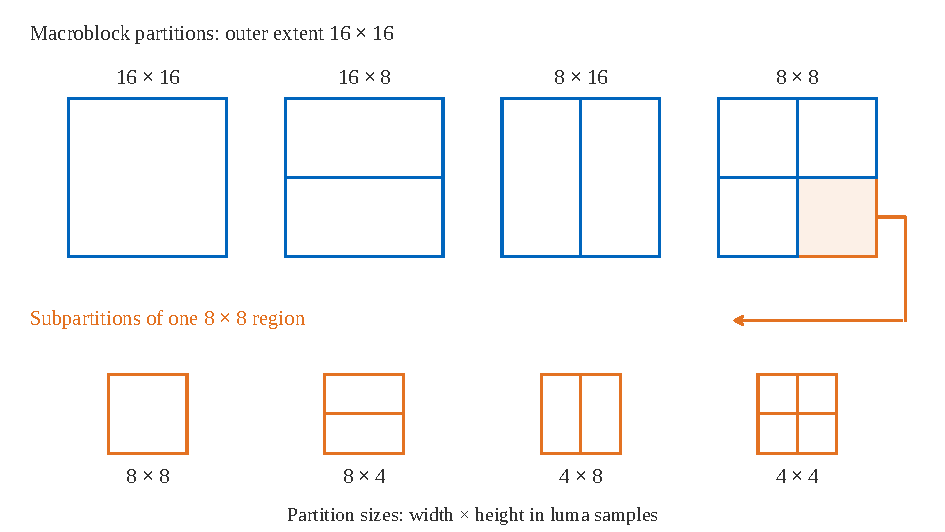
\includegraphics[width=\textwidth]{figures/background/h264-prediction-partitions}
  \caption[H.264 inter-prediction partitions]{H.264 inter-prediction partition choices in luma samples. Top:
  partitioning of a $16\times16$ macroblock. Bottom: possible subdivisions of
  one $8\times8$ region; the four regions of a partitioned macroblock can
  select these independently. The drawing uses a common spatial scale and
  shows prediction support, not transform blocks. Based on
  \cite[Tables~7-13 and~7-17]{ITUT_H264_2026}.}
  \label{fig:h264-prediction-partitions}
\end{figure}

Each inter-predicted partition or subpartition carries a translational motion
description, with one vector for a unidirectionally predicted block. Larger
partitions reduce the motion information to encode; smaller ones can represent
different displacements within the same macroblock at greater signalling cost.
These regions are not feature detections or object segments. Their selection
can change between pictures without preserving any identity
\cite[Sec.~IV-H]{Wiegand2003Overview}.

Prediction support must also be distinguished from residual transform size.
For example, the $4\times4$ transform operates on prediction-error samples; it
does not imply that every inter-prediction vector belongs to a $4\times4$
region. High-profile coding additionally permits an $8\times8$ transform
\cite[Secs.~8.5 and~A.2.4]{ITUT_H264_2026}. The MV block dimensions describe
where a displacement is applied, not the precision with which a point inside
that region has been localized.

\subsection{Reference Pictures and Temporal Direction}

Pictures are divided into slices, whose types constrain the available coding
modes. An I slice uses intra coding. A P slice permits intra coding and
inter prediction from one reference list; a B slice additionally permits a
prediction combining two reference lists. P and B slices can therefore contain
intra-coded regions with no inter-picture motion vector
\cite[Table~7-10]{ITUT_H264_2026}. The common terms I-, P-, and B-frame are
shorthand; a P label alone does not imply a temporal vector at every location.
An instantaneous decoding refresh (IDR) picture also resets reference-picture
dependencies. An ordinary intra-coded picture does not necessarily prevent
later pictures from referring to pictures preceding it
\cite[Sec.~3.69]{ITUT_H264_2026}.
A pattern such as I-P-P specifies coding types, but does not by itself specify
every reference relationship~\cite[Secs.~7.4.5 and~8.2.4]{ITUT_H264_2026}.

A vector is meaningful only together with its reference-picture identity.
H.264 can retain multiple reconstructed references, and decoding order need
not equal display order. In B prediction, either reference list can contain
pictures from either temporal direction; a list index is not by itself a
timestamp or a direction of motion
\cite[Secs.~IV-H.1 and~IV-H.2]{Wiegand2003Overview}.

The direction convention matters. Under a current-to-reference lookup
convention, a vector $\mathbf{m}$ pairs a location $\mathbf{q}$ in the current
coding block with $\mathbf{q}+\mathbf{m}$ in the reference
image~\cite[Sec.~3.95]{ITUT_H264_2026}. If the reference
is the preceding frame, forward-time propagation instead maps a point
$\mathbf{p}$ in that reference support to $\mathbf{p}-\mathbf{m}$. Thus an encoder
reference arrow and a forward-time motion arrow have opposite directions in
this case. For example, a horizontal lookup displacement of $-2$ pixels describes
a forward-time displacement of $+2$ pixels between those supports. It is a
displacement over the reference interval, not a velocity.

The experiments restrict reference count and prediction structure to simplify
this interpretation (\autoref{chapter:experimental-methodology}). Encoding the
same images in reverse order is nevertheless a new prediction problem, not a
way to obtain the exact inverse of the original vectors. This independently
encoded reverse stream is also distinct from the two reference lists of a
single B slice. Neither codec syntax nor rate-distortion optimization enforces
reciprocal agreement between the two encodings.

\subsection{Subpixel Precision and Decoded Motion Information}

H.264 represents luma motion in quarter-sample units. An integer vector
component $k$ therefore represents $k/4$ luma pixels, allowing displacements
between recorded sample locations. Motion compensation obtains these
fractional reference samples by interpolation: half-sample luma positions use
a six-tap filter, and quarter-sample positions use rounded averages of suitable
integer- and half-sample values
\cite[Secs.~8.4.2.2 and~8.4.2.2.1]{ITUT_H264_2026}. In 4:2:0 chroma, the
same displacement corresponds to eighth-chroma-sample units because that grid
has half the luma resolution; this does not provide eighth-pixel precision on
the luma image~\cite[Sec.~8.4.1.4]{ITUT_H264_2026}.

Fractional precision specifies representable displacements, not a bound on
error relative to physical image motion. The chosen vector is the result of
prediction search and coding decisions, not necessarily a correctly estimated
continuous motion rounded to its nearest quarter pixel. Consequently,
$0.25$-pixel representation alone justifies neither subpixel correspondence
accuracy nor a particular statistical uncertainty model.

The bitstream usually codes a motion-vector difference relative to a predicted
vector. For each component, reconstruction has the form
\begin{equation}
  \mathbf{m}=\mathbf{m}_{\mathrm{pred}}+\Delta\mathbf{m},
\end{equation}
where the predictor depends on neighbouring motion information, partition
shape, and reference indices
\cite[Sec.~8.4.1, Eqs.~(8-172) and~(8-173)]{ITUT_H264_2026}. A zero coded
difference is therefore not necessarily a zero displacement. The codec's
neighbour-based prediction, which includes median-based cases, saves bits;
it is separate from the motion-vector outlier filter introduced in
\autoref{chapter:method}.

Skip and direct modes provide another important distinction. A skipped P
macroblock has inferred motion information despite carrying no explicit
motion-vector difference or residual. Its derived vector need not be zero.
B direct and skip modes likewise derive motion from other decoded information
\cite[Secs.~8.4.1.1 and~8.4.1.2]{ITUT_H264_2026}. This differs from intra
coding, which provides no inter-picture vector. Extracting motion therefore
requires syntax parsing and reconstruction of motion information, including
inferred modes and reference identities, not simply reading explicit vector
differences. The standard separates this derivation from the subsequent use of
reference intensities for motion compensation
\cite[Secs.~8.4.1 and~8.4.2]{ITUT_H264_2026}. The estimator in this thesis
uses the resulting metadata, not the reconstructed intensity samples; this
does not mean that no compressed syntax is decoded.

\subsection{Motion Vectors versus Optical Flow and Feature Tracks}

Optical flow describes apparent image motion between images. A common local
model seeks a displacement $\mathbf{f}$ satisfying brightness constancy,
\begin{equation}
  I_{t+1}(\mathbf{u}+\mathbf{f}(\mathbf{u}))\approx I_t(\mathbf{u}),
\end{equation}
with spatial assumptions or patch support resolving otherwise ambiguous
matches. KLT uses such image information to refine a point displacement;
texture is needed to constrain that displacement in both directions
\cite{shi1994good,young2020fast}. Occlusion, changing illumination, repeated
patterns, and the aperture problem still limit optical-flow estimates: an
isolated straight edge does not constrain displacement along its own direction.
Optical flow is therefore not synonymous with ground-truth scene
correspondence.

Codec motion and optical flow are related because both exploit displaced image
appearance. Their objectives and outputs differ. Codec prediction trades
distortion against coded bits, may use a non-adjacent reference, and assigns one
translation to an entire prediction region. It can leave mismatched appearance
to the coded residual. Optical-flow estimation instead seeks an image-motion
field, without a cost for encoding its vectors in an H.264 stream. Repeating a
block vector at every covered pixel produces a dense array, but adds no
independent motion measurements or localized features. A useful prediction of
the block's appearance can therefore differ from the motion of a particular
corner or edge inside it~\cite{young2020fast,hilscher2026voca}.

\begin{figure}[htbp]
  \centering
  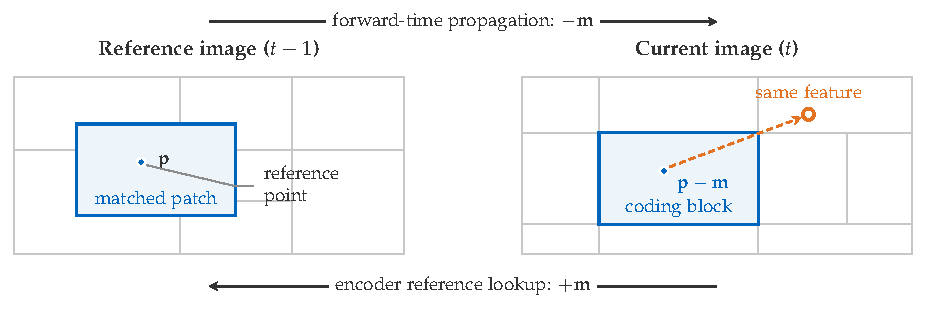
\includegraphics[width=\textwidth]{figures/background/mv-block-prediction}
  \caption[Block prediction and physical feature motion]{Conceptual block prediction, not measured data. Blue rectangles
  mark a matched reference patch and its current coding block. Applying their
  displacement to the reference point produces the filled blue point; the
  same physical feature may appear elsewhere (orange ring). Gray lines show
  independently chosen coding partitions. The arrows distinguish encoder
  reference lookup from chronological propagation for an earlier reference.}
  \label{fig:mv-block-prediction}
\end{figure}

As illustrated in \autoref{fig:mv-block-prediction}, translating a point with
its containing block does not establish feature identity. A matched reference
patch need not coincide with a coding partition in the reference image.
Although coding partitions cover the current picture, their displaced
reference supports can overlap and leave gaps. Repeatedly selecting a block
that covers a propagated point can consequently switch the image structure
being followed. Conversely, a visible structure may have no usable vector:
its region may be intra-coded, or no available source support may cover the
queried point. Missing support supplies no motion measurement and does not
imply that the point is stationary. Measured examples of departure from a KLT
track and abrupt loss of local support are given in
\autoref{fig:mv-feature-departure-example} and
\autoref{fig:mv-abrupt-stop-example}.

Even the presence of a syntactically valid vector does not guarantee a valid
geometric observation. H.264 permits reference lookup outside the image by
extending boundary samples~\cite[Sec.~IV-H.1]{Wiegand2003Overview}; those
extended samples do not constitute additional observed scene content. This
motivates separating codec validity from the image bounds and rectification
validity required for the geometry used here.

\subsection{Texture and the Motion-Matching Error Surface}

The reliability of a block displacement also depends on the shape of its local
matching-error surface. Zhang et al.~\cite{zhang2010subpixel} characterize this
surface from the nine integer-pixel displacements centred on an integer-pixel
optimum. For an image-matching distortion expressed as a sum of squared
differences, the local surface is
\begin{equation}
  E(\Delta x,\Delta y)
  = \sum_{(x,y)\in W}
    \left[s(x,y)-c(x+d_{0x}+\Delta x,y+d_{0y}+\Delta y)\right]^2,
  \label{eq:mv-error-surface}
\end{equation}
where $s$ is the current block, $c$ is the reference image, $W$ is the
block support, and $\mathbf d_0$ is the selected integer-pixel displacement.
The perturbation $(\Delta x,\Delta y)$ is measured around that displacement.
With the first-order brightness-constancy approximation
\begin{equation}
  c(x+d_{0x}+\Delta x,y+d_{0y}+\Delta y)
  \approx c(x+d_{0x},y+d_{0y})+I_x\Delta x+I_y\Delta y,
\end{equation}
where $I_x$ and $I_y$ are evaluated at the corresponding reference location
for each pixel in $W$, the displacement Hessian is
\begin{equation}
  \mathbf{H}_E
  \approx 2\sum_{(x,y)\in W}
  \begin{bmatrix}
    I_x^2 & I_xI_y \\
    I_xI_y & I_y^2
  \end{bmatrix}
  =2\mathbf{M}_W.
  \label{eq:mv-error-hessian}
\end{equation}
Thus the local quadratic curvature is, up to a factor of two, the same
second-moment matrix used by Shi-Tomasi corner selection~\cite{shi1994good}.
A corner-like region supplies curvature in two displacement directions; an
edge leaves one direction weakly constrained, and a low-texture region leaves
both weakly constrained. Zhang et al. use the Hessian condition and deviation
from flatness to characterize the accuracy available to sub-pixel motion
estimation. This local SSD model explains matching ambiguity; it is not a
claim that every H.264 encoder minimizes SSD or uses this quadratic fit.
Under the rate-distortion tradeoff in \autoref{eq:codec-rate-distortion}, a
flat image-matching surface gives the rate term greater opportunity to affect
which displacement is selected. This is an interpretation of the local model,
not a guarantee that the chosen displacement represents physical point motion.
Empirical comparisons likewise show that codec vectors can deviate substantially
from refined optical flow in regions with
little texture, repetitive patterns, or strong motion
blur~\cite{hilscher2026voca}.

This relationship motivates using corner coincidence as an offline diagnostic
of whether a codec block contains structure capable of localizing translation.
It is not a correctness test for an individual vector: the actual codec surface
depends on two frames, interpolation, partitioning, and rate-distortion search,
and even a textured block can be assigned to the wrong physical surface.

This distinction accounts for the principal measurement difficulties considered later: block support is spatially quantized, several scene structures can contribute to one block, different blocks can describe nearly indistinguishable observations, and useful temporal information can be absent at intra-coded regions.

\section{Robust Point-Cloud Registration}

Rigid registration estimates a rotation $\mathbf{R}\in\mathrm{SO}(3)$ and translation $\mathbf{t}\in\mathbb{R}^3$ from putative 3D-3D correspondences $(\mathbf{a}_i,\mathbf{b}_i)$. Incorrect associations make ordinary least squares brittle. TEASER formulates robust registration with a truncated least-squares objective,
\begin{equation}
  \min_{\mathbf{R},\mathbf{t}}
  \sum_i \min\!\left(
    \frac{\lVert\mathbf{b}_i-(\mathbf{R}\mathbf{a}_i+\mathbf{t})\rVert^2}
         {\beta_i^2},
    \bar{c}^{\,2}
  \right),
\end{equation}
where $\beta_i$ bounds the expected inlier noise, $\bar c$ is the dimensionless truncation threshold, and the scale is fixed for metric point clouds~\cite{yang2020teaser}. Large residuals saturate instead of dominating the estimate. TEASER++ combines invariant measurements, graph-based outlier pruning, and graduated non-convexity to obtain a robust rigid transform and an inlier set.

CLIPPER addresses the related problem of selecting mutually consistent associations. It represents putative matches as vertices of a consistency graph and uses pairwise geometric compatibility to recover a dense inlier subgraph~\cite{lusk2021clipper}. This illustrates the distinction between proposing correspondences and validating them geometrically. The implementation in this thesis uses TEASER++, not CLIPPER: its pairwise transform filters stereo-temporal associations and supports identity propagation, but is not used as the reported camera trajectory.

\section{Trajectory Evaluation}

Let $\mathbf{T}_i$ and $\widehat{\mathbf{T}}_i$ be synchronized reference and estimated camera poses. Before evaluation, the estimate is brought into the reference frame with a rigid $\mathrm{SE}(3)$ alignment $\mathbf{S}$ obtained from corresponding positions~\cite{umeyama1991least}. The absolute pose error is
\begin{equation}
  \mathbf{E}_i = \mathbf{T}_i^{-1}\mathbf{S}\widehat{\mathbf{T}}_i,
\end{equation}
and absolute trajectory error (ATE) is the root mean square of $\lVert\operatorname{trans}(\mathbf{E}_i)\rVert$ over the trajectory~\cite{sturm2012benchmark}. It measures global disagreement after alignment and is therefore sensitive to accumulated drift.

Relative translation error compares motion over a fixed interval $\Delta$. Its pose error is
\begin{equation}
  \mathbf{F}_i^{\Delta}
  = \left(\mathbf{T}_i^{-1}\mathbf{T}_{i+\Delta}\right)^{-1}
    \left(\widehat{\mathbf{T}}_i^{-1}\widehat{\mathbf{T}}_{i+\Delta}\right),
\end{equation}
with the translational statistic computed from $\operatorname{trans}(\mathbf{F}_i^{\Delta})$~\cite{sturm2012benchmark}. It describes local drift over the chosen interval rather than global trajectory agreement, so it need not rank methods in the same order as ATE. The alignment and interval used in the experiments are specified in \autoref{chapter:experimental-methodology}.

% !TeX root = ../main.tex

\chapter{Related Work}\label{chapter:related-work}

\section{Compression and the Placement of Visual Analysis}

Compress-then-analyze and analyze-then-compress allocate different work to a
capturing device and its receiver. Hofer et al.~\cite{hofer2023h264cta}
investigate H.264 transmission for edge-assisted visual SLAM, evaluating
encoding, transmission, decoding, and feature-analysis latency on a Raspberry
Pi and an Intel NUC. Their software OpenH264 experiments motivate transmitting
compressed video when capture-side feature extraction is costly; they evaluate
the coding pipeline independently of a complete SLAM system and do not measure
energy consumption.

Redondi et al.~\cite{redondi2016cta} compare JPEG-based CTA and BRISK-feature ATC
for image recognition in visual sensor networks. Their measurements and network
evaluation relate recognition accuracy, transmission rate, and camera-node
energy. The outcome depends on the hardware, feature workload, and link
constraints. These studies motivate the allocation of visual computation; the
present thesis investigates what the receiver can infer directly from codec
motion without a pixel-based correspondence stage.

\section{Motion-Vector Refinement into Optical Flow}

Young, Girod, and Taubman~\cite{young2020fast} recover a dense optical-flow field from block-based coded motion using confidence-weighted filtering and inpainting. Prediction-unit dimensions inform the confidence model, while decoded image colours guide edge-preserving filtering; optional variational refinement additionally uses image gradients, temporal intensity differences, and warping. This work characterizes how codec motion can initialize a more accurate flow estimate, but its recovered flow is a pixel-guided product rather than a codec-only geometric observation.

\section{Codec-Aware Tracking}

VOCA~\cite{hilscher2026voca} uses H.264 motion vectors as initialization priors
for KLT tracking. The codec prediction moves the initial estimate closer to the
subsequent photometric solution, while KLT refinement and conventional tracking
modes retain access to decoded image intensities. VOCA provides the implementation
context and the reference configurations used in this thesis, but does not
impose the same pixel-access restriction.

\section{Motion Vectors for Camera Motion and Mapping}

Li and Song~\cite{li2014toward} estimate monocular camera motion and planar scene
structure from MPEG motion vectors. Their formulation explicitly assumes a
structured environment dominated by planes, such as building facades and paved
roads. It merges direct and bidirectional-frame observations, rejects
insufficient-parallax motion, groups correspondences with homography RANSAC, and
jointly tracks planes and camera motion in an extended Kalman filter. It thus
establishes an early codec-only navigation result within this planar setting,
rather than a general point-based reconstruction. Its B-frame observations also
depend on subsequent anchor images: they cannot be formed as soon as each
intermediate image is captured, introducing buffering and latency for a live
camera. The paper does not establish end-to-end real-time operation. These
constraints concern both the required scene structure and the availability of
the measurements, independently of the estimator's computational cost.

MoV-SLAM~\cite{turner2023movslam} uses H.264 macroblocks and their motion vectors to build long-range correspondence tracks within a complete monocular and stereo SLAM system. Its EXPRESS detector evaluates block intensities to select distinctive regions, while Lucas-Kanade tracking handles missing motion-vector coverage and stereo association. It consequently demonstrates how codec motion can reduce frontend cost without enforcing the pixel-access boundary studied here.

\section{Motion Vectors for Correspondence and Reconstruction}

Zouein et al.~\cite{zouein2025leveraging} convert AV1 block centres and motion vectors into point correspondences, propagate them into multi-frame tracks, and reject directionally inconsistent tracks using cosine similarity. Their evaluation focuses on correspondence density, pairwise geometry, and a small COLMAP structure-from-motion demonstration rather than a dedicated visual-odometry estimator.

The subsequent Gaussian-splatting work~\cite{zouein2026efficient} reuses this
correspondence pipeline to produce dense COLMAP point clouds for initializing 3D
Gaussian splatting. It evaluates the effect of denser reconstruction on
rendering quality and training time, without introducing calibrated stereo depth
or a motion-vector-specific visual-odometry backend.

\section{Motion-Vector Stereo}

Passthrough+~\cite{chaurasia2020passthrough} repurposes video-encoding hardware
to estimate correspondences between rectified views of a stereo pair. Shifted
copies of the stereo images reduce the displacement presented to the encoder
and offset the codec block grid, after which consistency checks and calibrated
triangulation produce sparse 3D points. This per-frame stereo stage uses codec
motion, but the complete scene proxy is not motion-vector-only: the system
assumes a high-precision headset pose, typically supplied by an independent
SLAM system, and uses pose to propagate the previous depth map into the current
view. That pose-assisted temporal model is unavailable under the information
restriction of this thesis. The present work adapts the sparse
stereo-reconstruction principle; the differences in preprocessing and downstream
use are specified in \autoref{chapter:method}.

\section{Spatial Feature Management}

Feature-based estimators generally regulate both the number and spatial
distribution of their observations. VINS-Mono maintains a target population of
corner tracks and enforces a minimum separation between newly detected features
to obtain a more uniform distribution~\cite{qin2018vins}. Similarly, the
low-latency VIO pipeline of K\"uhne et al. suppresses nearby detector candidates
so that the same local feature is not represented repeatedly~\cite{kuhne2025lowlatency}.
Both systems make these decisions from image-derived features. Their common
design objective motivates the pixel-free analogue developed here: codec
observations that are indistinguishable at the available spatial and depth
resolution should not provide duplicated geometric support.

\section{Positioning of This Work}

The compressed-domain systems above span the distinctions central to this thesis: whether
codec motion is refined using pixels, whether recovered structure is planar or
point-based, whether metric scale is supplied by stereo, and whether
correspondences persist beyond a frame pair. Work that merely accelerates video
decoding or generic optical flow without using codec side information is outside
this comparison.

Prior codec-only navigation establishes that motion vectors can support
camera-motion estimation in structured, plane-dominated
environments~\cite{li2014toward}. Other work uses codec motion to initialize
pixel-domain tracking or provide correspondences for reconstruction. The present
work investigates one way to use these measurements in a calibrated, point-based
stereo visual-odometry system without requiring a planar scene model. The
evaluated design combines metric motion-vector stereo, persistent 3D
association, suppression of geometrically indistinguishable observations, and
displacement-based optimization without pixel refinement. Its reverse-temporal
streams are nevertheless prepared offline, so this study also leaves causal,
end-to-end real-time operation unverified.

\begin{table}[p]
  \centering
  \caption[Comparison of compressed-domain visual methods]{Comparison of directly related compressed-domain systems. ``Pixels''
  refers to image-intensity access in correspondence generation or geometric
  estimation, not to the image input required by an encoder.}
  \label{tab:related-work-comparison}
  \begingroup
  \footnotesize
  \setlength{\tabcolsep}{1mm}
  \begin{tabular}{@{}L{26mm}L{29mm}L{24mm}L{36mm}L{25mm}@{}}
    \toprule
    Work & Input and representation & Scale and pixel access &
    Track persistence and validation & Estimator or output \\
    \midrule
    Young et al.~\cite{young2020fast}
      & Coded MVs\newline Dense 2D flow
      & No scale\newline Pixels used
      & \textit{Persistence:} none\newline \textit{Validation:} pairwise confidence
      & Pixel-guided flow \\
    Li and Song~\cite{li2014toward}
      & MPEG MVs\newline Planes and pose
      & Monocular\newline No pixels
      & \textit{Persistence:} plane tracks\newline \textit{Validation:} homography RANSAC
      & Extended Kalman filter \\
    MoV-SLAM~\cite{turner2023movslam}
      & H.264 MVs and LK\newline Point tracks
      & Mono/stereo\newline Pixels used
      & \textit{Persistence:} point tracks\newline \textit{Validation:} LK fallback
      & SLAM backend \\
    Zouein et al.~\cite{zouein2025leveraging}
      & AV1 MVs\newline 2D point tracks
      & Monocular\newline No pixels
      & \textit{Persistence:} MV tracks\newline \textit{Validation:} directional check
      & Matching and SfM study \\
    Zouein et al.~(2026)~\cite{zouein2026efficient}
      & AV1 MVs\newline Dense 3D points
      & Monocular SfM\newline Pixels downstream
      & \textit{Persistence:} MV tracks\newline \textit{Validation:} geometric checks
      & COLMAP and 3DGS \\
    VOCA~\cite{hilscher2026voca}
      & H.264-seeded KLT\newline Point tracks
      & Calibrated VO\newline Pixels used
      & \textit{Persistence:} KLT tracks\newline \textit{Validation:} fallback modes
      & Sliding window BA \\
    Passthrough+~\cite{chaurasia2020passthrough}
      & Stereo encoder MVs and SLAM pose\newline Sparse depth and dense proxy
      & Metric stereo\newline Pixels used
      & \textit{Persistence:} temporal depth\newline \textit{Validation:} stereo consistency
      & View synthesis \\
    Pixelless VO (this thesis)
      & H.264 temporal and stereo MVs\newline Persistent 3D points
      & Metric stereo\newline No estimator pixels
      & \textit{Persistence:} landmark IDs\newline \textit{Validation:} reciprocal + TEASER++
      & Sliding window BA \\
    \bottomrule
  \end{tabular}
  \endgroup
\end{table}

No row alone defines the contribution. In particular, codec-only navigation
predates this thesis, motion-vector tracks have already been used for
reconstruction, and motion-vector stereo originates in Passthrough+. The present
study tests how these ingredients behave together under a pixel-free estimation
boundary and within a point-based visual-odometry estimator.

% !TeX root = ../main.tex

\chapter{Compressed-Domain Visual Odometry}\label{chapter:method}

\section{System Overview}

The examined pipeline separates image-dependent preparation from compressed-domain
estimation, as summarized in \autoref{fig:system-pipeline}. Offline preparation
encodes native images into temporal H.264 streams and rectified images into
stereo streams. The extraction software decodes these streams to obtain their
motion-vector metadata. Only codec side information, calibration, masks, and
timing metadata enter the tracking frontend and pose estimator.
Temporal vectors propose motion, shifted stereo encodings provide metric
depth, and robust registration validates the resulting 3D-3D associations.
Confirmed identities are converted into observations for a windowed
visual-odometry backend.

\begin{figure}[htbp]
  \centering
  \resizebox{\textwidth}{!}{%
  \begin{tikzpicture}[
      prep/.style={draw=TUMBlue, rounded corners, align=center, fill=white,
        minimum height=9mm, text width=25mm, font=\small},
      estimation/.style={draw=TUMBlue, rounded corners, align=center, fill=white,
        minimum height=10mm, text width=22mm, font=\small},
      flow/.style={->, thick, color=TUMDarkGray}]
    \node[anchor=west,font=\small\bfseries,color=TUMSecondaryBlue]
      at (-0.35,4.55) {Offline preprocessing: image intensities available};
    \draw[dashed,rounded corners,color=TUMSecondaryBlue]
      (-0.50,0.45) rectangle (13.05,4.35);

    \node[prep] (images) at (1.00,2.35) {Native stereo images\\and calibration};
    \node[prep] (temporal) at (4.35,3.35) {Temporal H.264\\forward and reverse};
    \node[prep] (rectify) at (4.35,1.35) {Rectification\\+ masks};
    \node[prep] (stereoencode) at (7.75,1.35) {Shifted stereo H.264\\I-P-P streams};
    \node[prep] (products) at (11.45,2.35) {Encoded streams,\\masks +\\calibration};
    \draw[flow] (images.east) -- ++(0.35,0) |- (temporal.west);
    \draw[flow] (images.east) -- ++(0.35,0) |- (rectify.west);
    \draw[flow] (rectify) -- (stereoencode);
    \draw[flow] (temporal.east) to[out=0,in=90] (products.north);
    \draw[flow] (stereoencode.east) to[out=0,in=-90] (products.south);

    \node[anchor=west,font=\small\bfseries,color=TUMSecondaryBlue]
      at (-0.35,0.05) {Frontend and pose estimation: no image intensities};
    \draw[dashed,rounded corners,color=TUMSecondaryBlue]
      (-0.50,-3.00) rectangle (10.10,-0.15);
    \node[prep] (extract) at (11.65,-1.60) {Decode frames +\\extract MV metadata\\(uses pixels)};
    \node[estimation] (filter) at (8.80,-1.60) {Median + reciprocal\\filtering};
    \node[estimation] (stereolookup) at (6.15,-1.60) {Stereo depth\\at both\\endpoints};
    \node[estimation] (registration) at (3.50,-1.60) {TEASER++ +\\track identity};
    \node[estimation] (backend) at (0.85,-1.60) {Suppression +\\rigid-flow BA};
    \draw[flow] (products.south) -- (extract.north);
    \draw[flow] (extract) -- (filter);
    \draw[flow] (filter) -- (stereolookup);
    \draw[flow] (stereolookup) -- (registration);
    \draw[flow] (registration) -- (backend);
  \end{tikzpicture}}
  \caption[Processing pipeline and pixel-access boundary]{Processing pipeline and pixel-access boundary. Rectification and
  both H.264 paths operate on images before evaluation. Native images feed the
  forward/reverse temporal encodings, while rectified images feed the shifted
  stereo encodings. The extractor reconstructs image pixels, which are not
  passed to the frontend. The pixel-free boundary encloses correspondence
  filtering, stereo lookup, association, and pose estimation; these stages
  consume only side information, masks, timing data, and calibrated geometry.}
  \label{fig:system-pipeline}
\end{figure}

\section{Input and Pixel-Access Boundary}

For each timestamp, the estimator receives temporal motion vectors from the
forward and reverse encodings, stereo motion vectors from the shifted I-P-P
encodings, the width and height of every prediction block, reference direction,
fractional displacement and frame type. It additionally receives the two-camera
calibration, synchronized timestamps, the virtual rectification model, and the
two rectification validity masks. These quantities are sufficient to express
codec supports in native camera coordinates and to form calibrated rays.

In compressed-domain operation, image loading is disabled before observations
enter the frontend. The frontend neither constructs image pyramids nor
runs FAST, KLT, patch alignment, descriptor extraction, or a photometric test.
Image intensities are used to generate the H.264 streams during offline
preprocessing, and the extraction software reconstructs images while reading
codec side information. Neither the tracking frontend nor pose estimation consumes
those intensities. The Shi-Tomasi and blur measurements reported later
are likewise post-hoc diagnostics and are not available to pose estimation.

\section{Stereo Rectification and Video Preprocessing}

Rectification is constructed separately for each supplied stereo calibration.
The camera supplying temporal track candidates is designated the anchor camera
$A$, and the other view is the stereo camera $S$. Let
${}^{A}\mathbf{t}_{S}$ be the position of the stereo camera expressed in the
anchor-camera frame.
The horizontal axis of the virtual camera is
$\mathbf{e}_x={}^{A}\mathbf{t}_{S}/\lVert{}^{A}\mathbf{t}_{S}\rVert$.
The sum of the two native optical axes, expressed in the anchor-camera frame,
is projected onto
the plane orthogonal to $\mathbf{e}_x$ and normalized to form
$\mathbf{e}_z$; $\mathbf{e}_y=\mathbf{e}_z\times\mathbf{e}_x$ completes the
orientation. This produces a common view direction while making the calibrated
baseline horizontal.

Both cameras are remapped into the same undistorted pinhole projection. Its
resolution equals the native EuRoC resolution, its principal point is the image
centre, and its common focal length is the smallest of the four native horizontal
and vertical focal parameters. Each virtual ray is rotated into the respective
native camera and projected with that camera's calibrated distortion model.
Bilinear sampling produces the offline rectified images. Pixels for which this
mapping is invalid are set to zero, and a binary validity mask for each camera is
stored with the virtual intrinsics and rotations. During estimation, an entire
codec block is rejected if either of its rectified supports intersects an invalid
region.

Camera streams are paired by their recorded nanosecond timestamps. If one camera
contains an unmatched terminal image, only that unpaired timestamp is removed
from the longer metadata stream; both the temporal video and its reverse
counterpart are generated from the resulting ordered timestamp list. EuRoC has
two cameras, so its calibrated pair is used directly. For a dataset with more
than two cameras, one calibrated pair would have to be designated as the anchor
and stereo views; additional cameras would remain outside the
Passthrough+-derived depth stage.

\section{Codec-Domain Stereo Correspondences}

Only the sparse encoder-stereo stage of Passthrough+~\cite{chaurasia2020passthrough} is adapted. The shifted views are represented as independent full-frame encodings rather than subframes of one hardware-encoder mosaic. Temporal motion-search and partition settings are retained, while the reference structure, rate control, and encoded frame rate follow the stereo configuration in \autoref{chapter:experimental-methodology}. Each EuRoC camera pair is remapped into a calibration-specific common virtual projection before encoding. During estimation, stereo motion vectors are queried only at temporal candidate locations; their endpoints are converted back to native camera rays and triangulated with the calibrated baseline.

The original hemispherical depth grid, Laplacian densification, stereoscopic rendering, and pixel-based subpixel refinement are not used. Nor is its temporal depth-map propagation: Passthrough+ projects the previous depth map using a headset pose obtained from an independent SLAM system~\cite{chaurasia2020passthrough}, whereas no external pose estimate is available here. Sparse stereo depths instead serve as geometric support for temporal association and visual odometry.

Writing $L$ for the anchor view and $R$ for the stereo view, three horizontal
pre-shifts, 0, 8, and 32 pixels, are combined with four codec
grid phases, $(0,0)$, $(4,0)$, $(0,4)$, and $(4,4)$ pixels. The resulting twelve
independent streams contain repeated triples
\begin{equation}
  I(L_t^{s,g}),\quad P(R_t^g),\quad P(L_t^{s,g}),
\end{equation}
where $s$ denotes the disparity pre-shift and $g$ the grid phase. With one
reference frame, the first P-frame supplies left-to-right predictions and the
second supplies right-to-left predictions. The known artificial shifts are
removed from the reported block coordinates. Left-to-right and right-to-left
blocks are paired one-to-one when their supports overlap and their componentwise
cycle error is at most 1.0 pixel. The intersection of the two supports becomes
the validated rectangle.

A native anchor-camera query $\mathbf{u}$ is first unprojected, rotated into the virtual
frame, and projected onto the rectified grid. Every variable-sized codec block
whose source rectangle contains this location is considered; blocks are not
expanded into per-pixel points. Applying that block's fractional motion vector
gives a candidate in the rectified right view. Both endpoints must lie in valid
rectification support, and their vertical displacement in the common grid must
not exceed one pixel. The encoded right endpoint is then converted to a native
stereo-camera ray. The frontend triangulates distances along unit native-camera
bearings. Candidates are rejected when their calibrated epipolar error exceeds
$0.005$, triangulation is degenerate, either depth is at most
$\SI{0.333}{\metre}$, the anchor-camera depth exceeds $\SI{30}{\metre}$, or reprojection
into the stereo camera differs from the candidate by more than $1.5$ pixels.

When several encodings or overlapping variable-size blocks cover the query, one
stereo observation is returned. Its ranking cost is
\begin{equation}
  C = e_{\mathrm{repr}} + e_{\mathrm{epi}}
      + 10^{-4}wh + 10^{-3}d_c,
\end{equation}
Here $e_{\mathrm{repr}}$ is the stereo reprojection distance in pixels, and
$e_{\mathrm{epi}}=|\hat{\mathbf b}_L^{\mathsf T}\mathbf E\hat{\mathbf b}_R|$
is a dimensionless epipolar residual. The bearings are unit vectors in their
native camera frames, and $\mathbf E$ is the essential matrix formed from the
calibrated relative rotation and unit baseline direction.
The product $w h$ is block area and $d_c$ is the squared, block-size-normalized
distance from the query to the block centre. This preference resolves duplicate
codec hypotheses locally; the later suppression stage handles geometrically
indistinguishable temporal measurements.

\subsection{Grid Sampling and Disparity Pre-Shifts}

The grid phases and horizontal pre-shifts address two different aspects of
stereo correspondence. Grid phases increase spatial sampling density.
Applying the same phase $g$ to both views moves the codec's sampling grid
relative to the scene while preserving disparity. In the eight-pixel sampling
example used by Passthrough+~\cite{chaurasia2020passthrough}, the phases
$(0,0)$, $(4,0)$, $(0,4)$, and $(4,4)$ interleave into a grid with four-pixel
spacing in both directions, as shown in \autoref{fig:stereo-grid-interleaving}.
The combined samples refine spatial coverage. This spacing describes the
sampling construction; the encoded prediction blocks and their validated
intersections retain variable sizes.

\begin{figure}[htbp]
  \centering
  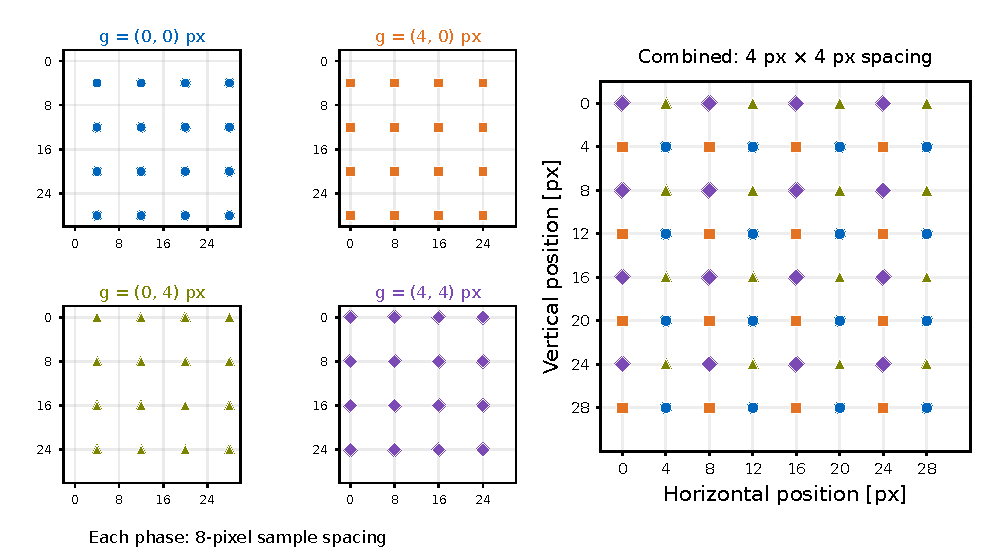
\includegraphics[width=\textwidth]{figures/method/stereo-grid-phase-interleaving.pdf}
  \caption[Finer spatial sampling through grid-phase interleaving]{Grid-phase interleaving, illustrated for an eight-pixel base grid.
  The four phases sample different positions in the same image coordinates.
  Their union has four-pixel spacing horizontally and vertically. Colour and
  marker shape identify the originating phase. The same phase is applied to
  both stereo views, so it changes sampling position without changing disparity.}
  \label{fig:stereo-grid-interleaving}
\end{figure}

Horizontal pre-shifts change the displacement presented to the encoder.
Passthrough+ reports that encoders favour short motion vectors, making
large disparities from nearby surfaces harder to recover~\cite{chaurasia2020passthrough}.
For disparity $d=u_L-u_R$, shifting the left image by $s$ pixels presents
$d-s$ to the encoder. The known shift is restored before triangulation.
With focal length $f_x$ and baseline $B$, rectified axial depth satisfies
\begin{equation}
  Z = \frac{f_x B}{d}, \qquad
  |d-s| = \left|\frac{f_x B}{Z}-s\right|.
  \label{eq:stereo-shift-depth}
\end{equation}
Here $Z$ is axial depth in the virtual rectified camera, used to interpret the
pre-shift examples and depth visualizations. The tracking frontend instead
triangulates distance along native-camera unit bearings, denoted $\lambda$
below.

\autoref{fig:stereo-shift-success-failure} shows two locations whose depth is
recovered by different pre-shifts. At the EMH01 location at \SI{135}{\second},
a disparity of 29.25 pixels gives $Z\approx\SI{1.31}{\metre}$. The 32-pixel
pre-shift reduces the required displacement to 2.75 pixels and provides an
accepted match. The displayed 0- and 8-pixel proposals instead have a vertical
error of 1.75 pixels and fail the one-pixel check. At the EMH02 location at
\SI{95}{\second}, disparity is 8.50 pixels and $Z\approx\SI{4.52}{\metre}$;
the 8-pixel pre-shift reduces the required displacement to 0.50 pixels and
supplies the depth.

For each location, all four grid phases are checked: neither of the other
pre-shifts returns an accepted block covering that query. Thus, a pre-shift
can determine whether a particular scene location supplies depth, and the
useful pre-shift changes with disparity. Local appearance and codec decisions
also affect availability, so useful depth ranges can overlap.
The illustrated matches pass rectification-mask, vertical-displacement,
reciprocal-cycle, and one-to-one overlap checks; they precede temporal tracking
and backend landmark selection. An overview of the correspondences from all
twelve transforms on a later EMH02 frame is given in
\autoref{fig:stereo-all-shifts}.

\begin{figure}[p]
  \centering
  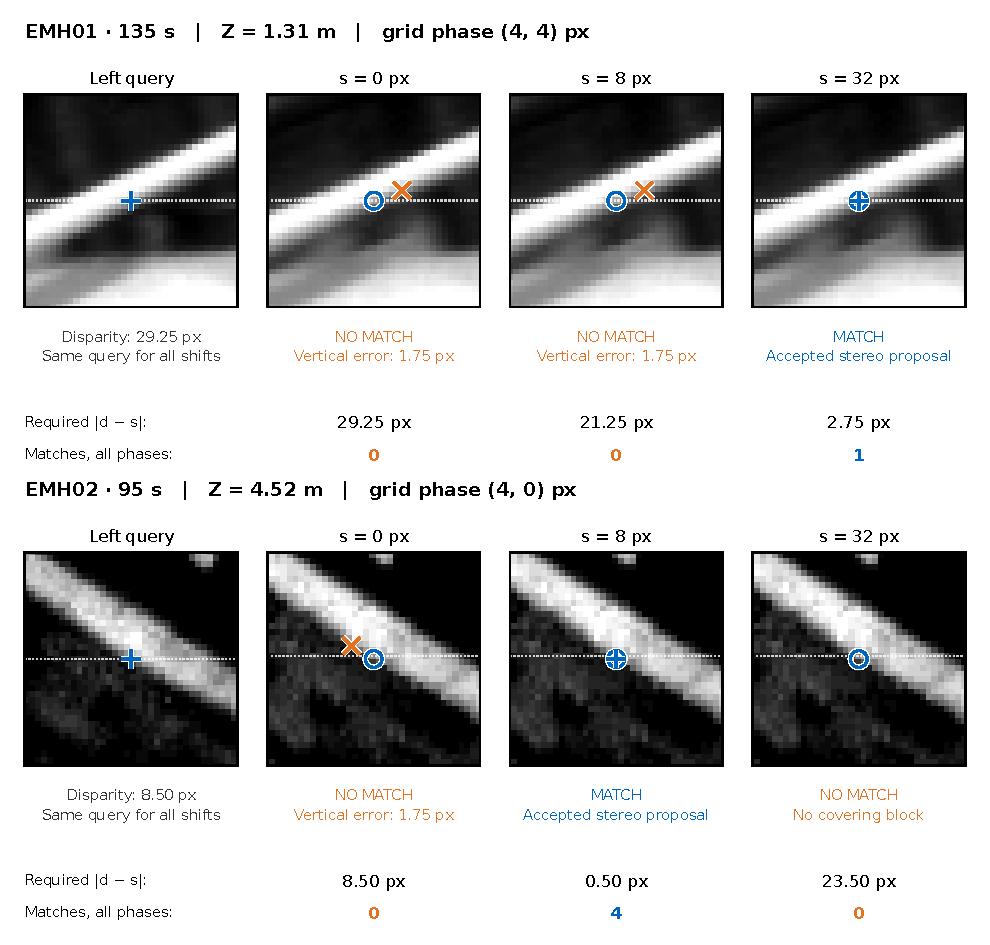
\includegraphics[width=\textwidth]{figures/method/stereo-shift-exclusive-depths.pdf}
  \caption[Depth recovery at different pixel pre-shifts]{Pre-shift-dependent depth recovery at two later scene locations.
  Each row holds the left query and displayed grid phase fixed. Blue circles
  repeat the right-image match supplied by the successful pre-shift; orange
  crosses mark rejected proposals. The dotted line is the query's epipolar
  row. The required residual $|d-s|$ is computed from the recovered disparity;
  the counts below include all four grid phases. Left and right crops within
  a row share one grayscale display scale.}
  \label{fig:stereo-shift-success-failure}
\end{figure}

\autoref{fig:stereo-depth-examples} and
\autoref{fig:stereo-depth-late-machine-hall} show depth renderings in three
scenes: EV101 at \SI{60}{\second}, EMH01 at \SI{115}{\second}, and EMH02 at
\SI{135}{\second}. A separate grayscale depth inset is placed inside each
rectified scene image. Stereo-block support surviving the rectification and
bidirectional checks is sampled on a four-pixel grid. Each supported sample
displays calibrated axial depth, using the median where several blocks cover
the same location. Brighter values indicate nearer surfaces; black marks
locations without a displayed sample. Unsupported regions are left unfilled.
These post-hoc renderings make the codec-derived geometry inspectable;
grayscale intensity is not passed to the estimator.

\begin{figure}[htbp]
  \centering
  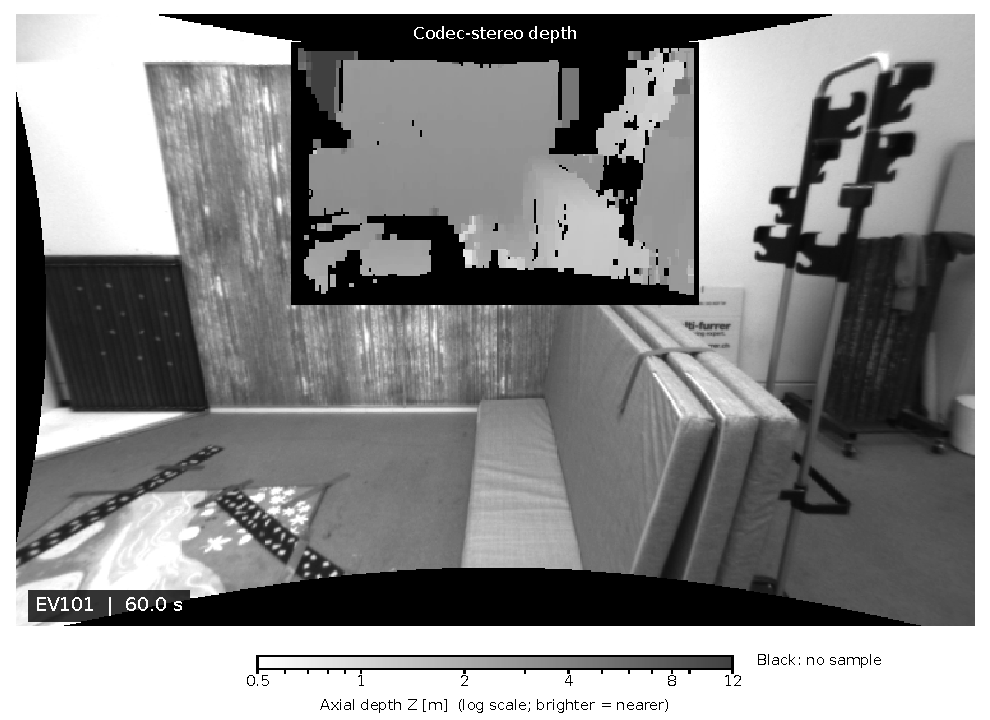
\includegraphics[width=\textwidth]{figures/method/depth-inset-ev101-f1200.pdf}
  \caption[Codec-stereo depth map on EV101]{Codec-stereo depth for EV101 at \SI{60}{\second}. The inset shows
  the full field of view on a four-pixel sampling grid, with nearer surfaces
  brighter on the logarithmic depth scale. Black marks unsupported samples;
  depths outside the displayed \SIrange{0.5}{12}{\metre} range are clipped
  only for grayscale visualization.}
  \label{fig:stereo-depth-examples}
\end{figure}

\begin{figure}[p]
  \centering
  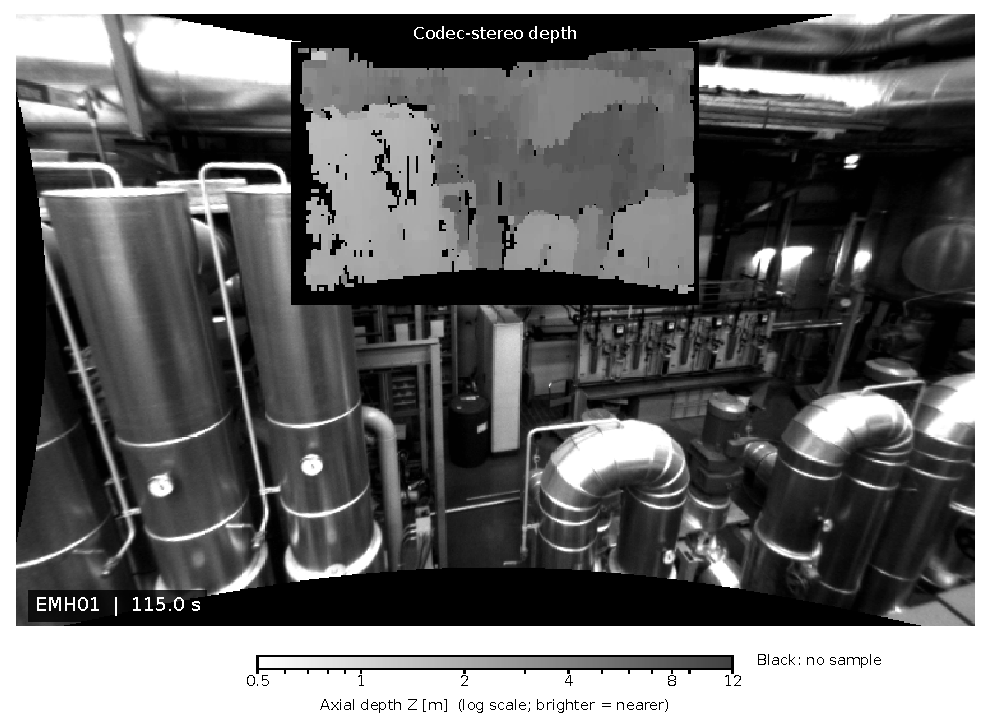
\includegraphics[width=0.80\textwidth]{figures/method/depth-inset-emh01-f2300.pdf}
  \par\medskip
  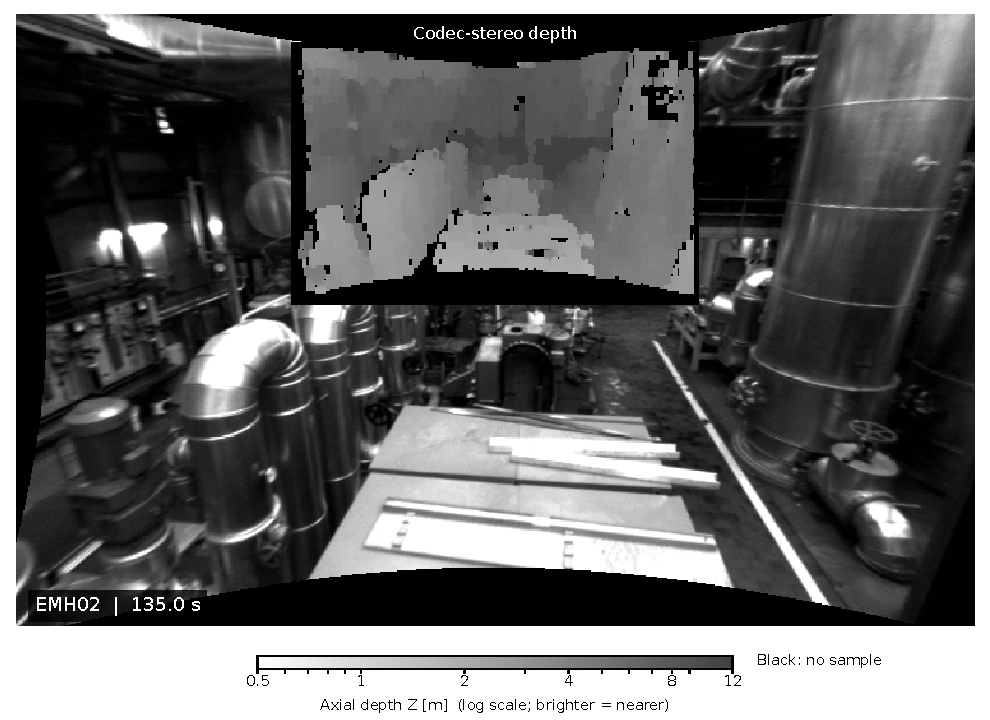
\includegraphics[width=0.80\textwidth]{figures/method/depth-inset-emh02-f2700.pdf}
  \caption[Codec-stereo depth maps in later Machine Hall scenes]{Additional codec-stereo depth maps in later Machine Hall scenes:
  EMH01 at \SI{115}{\second} (top) and EMH02 at \SI{135}{\second} (bottom).
  Both use the grayscale scale and sampling convention of
  \autoref{fig:stereo-depth-examples}. The separate depth insets distinguish
  nearby equipment from more distant structure while retaining unsupported
  regions in black.}
  \label{fig:stereo-depth-late-machine-hall}
\end{figure}

\section{Temporal Motion-Vector Candidates}

Motion vectors are read from the H.264 side data with their reference direction,
block dimensions, integer numerator, and scale. Only vectors referencing the
preceding encoded frame are used. Dividing the numerator by the scale preserves
the fractional current-to-reference displacement $\mathbf v$. In the forward
encoding, a coding-block centre $\mathbf q_t$ corresponds to the reference-support
centre $\mathbf q_{t-1}=\mathbf q_t+\mathbf v$. The temporal candidate runs from
$\mathbf q_{t-1}$ to $\mathbf q_t$, with forward displacement
$\mathbf m=-\mathbf v$. Later continuation may apply a covering block's
displacement to an established track location; it does not repeatedly snap that
location back to the block centre.

The compression-artifact filter tests local agreement without consulting the
image. Motion vectors are accumulated into a $16\times16$-pixel grid and their
two displacement components are averaged independently in each occupied cell.
For a cell $q$, let $\bar{\mathbf v}_q$ denote this mean and let
$\widetilde{\mathbf v}_q$ be the componentwise median of the occupied cells in
its $3\times3$ neighbourhood. Provided that at least three neighbouring cells
are occupied, every vector assigned to $q$ receives the score
\begin{equation}
  d_{\mathrm{med}}(q)
  = \left\lVert\bar{\mathbf v}_q-\widetilde{\mathbf v}_q\right\rVert_2.
\end{equation}
It is retained when $d_{\mathrm{med}}\leq5$ pixels. Border cells, cells without
sufficient neighbourhood support, out-of-image endpoints, and endpoints in
masked-out image regions are rejected. The result is illustrated in
\autoref{fig:median-filter-example}: the large magenta vectors disagree with
the coherent downward motion that dominates their neighbourhoods.

\begin{figure}[htbp]
  \centering
  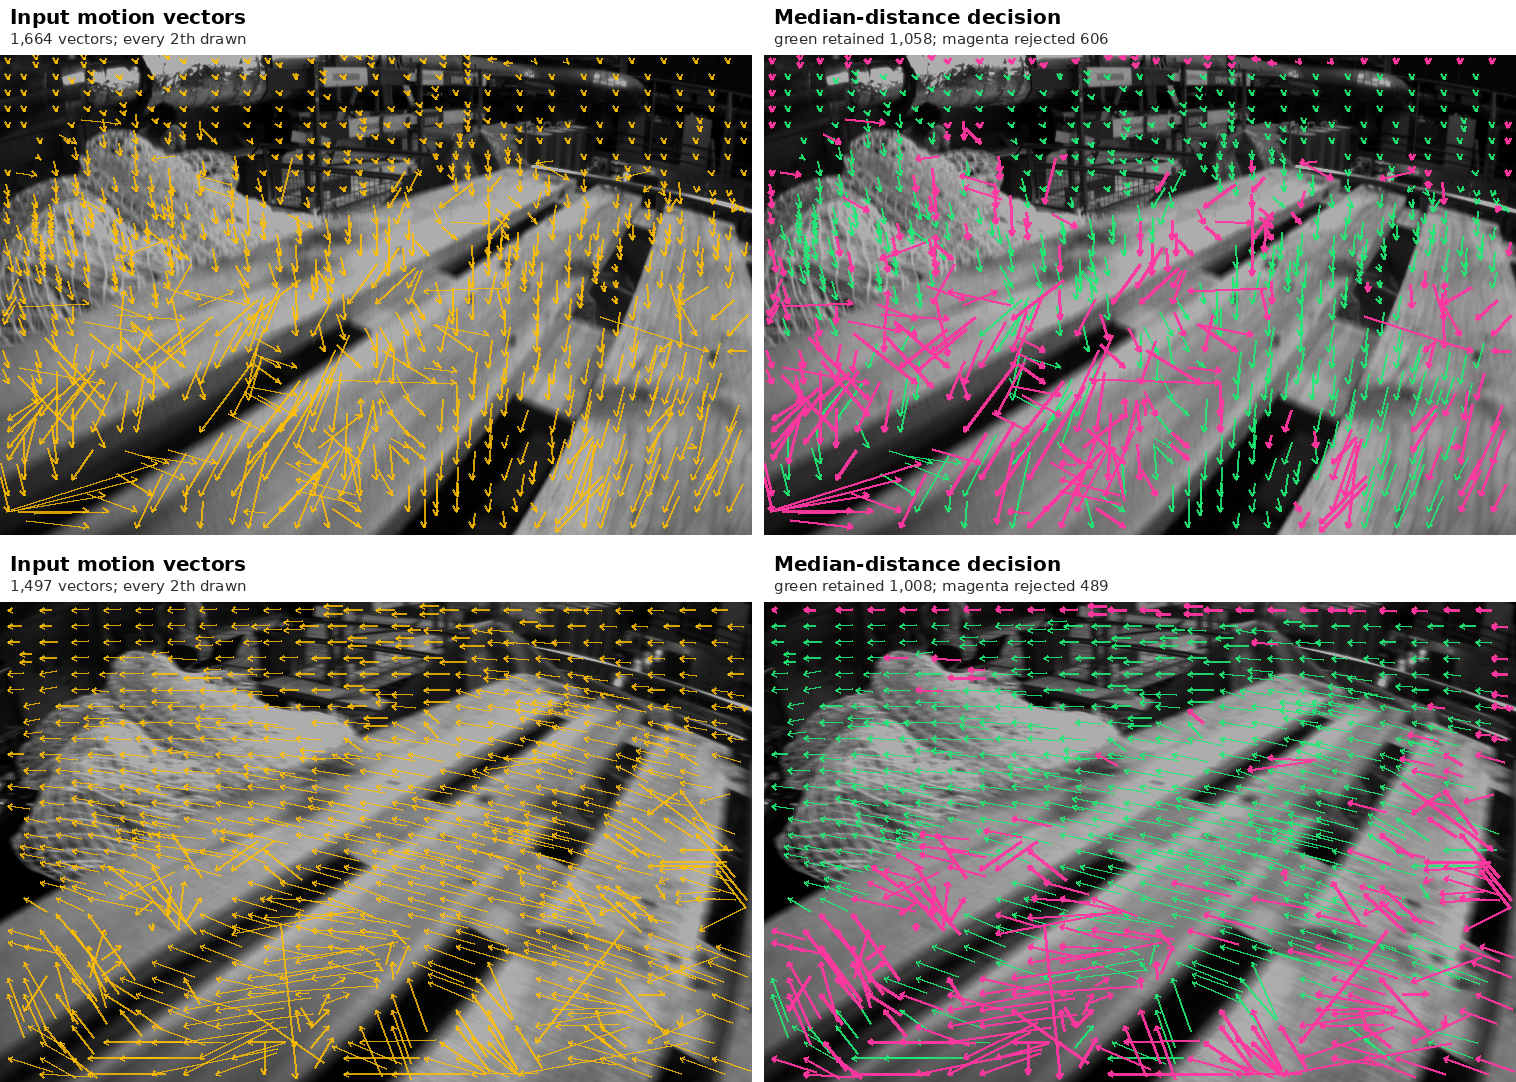
\includegraphics[width=\textwidth]{figures/method/median-filter-example}
  \caption[Median filtering of temporal motion vectors]{Examples of median-filter decisions on two EMH01 frames. In each row the
  left panel shows the input field; on the right, retained vectors are green and
  rejected vectors are magenta. Arrows use the measured displacements; dense
  populations are deterministically subsampled only for legibility.}
  \label{fig:median-filter-example}
\end{figure}

The forward encoding supplies $t-1\rightarrow t$ motion. A second video encoded
in reverse image order supplies the same interval from the opposite temporal
direction; its vectors and timestamps are inverted back into forward-time
coordinates. The fixed single-reference encoder setting prevents a temporal
vector from silently spanning more than one frame. At an I-frame boundary, the
available direction is used if exactly one encoding supplies inter prediction.
If neither direction supplies a candidate, the affected tracks terminate rather
than receiving a copied or pixel-derived displacement.

A motion vector describes a block prediction, not the identity of a scene point
inside that block. Naively assigning a persistent ID to whichever block covers
the previous sample can therefore fail in two distinct ways. First,
the selected block can continue to produce plausible motion after its displacement
has ceased to follow the same localized structure. \autoref{fig:mv-feature-departure-example}
shows this effect over fourteen transitions on a strong-gradient railing edge.
The codec path and a post-hoc KLT track initially agree, then separate
progressively while raw codec vectors remain available.

\begin{figure}[htbp]
  \centering
  \begin{minipage}[t]{0.485\textwidth}\centering
    \textbf{Track initialization}\\[-0.15em]
    {\small stereo depth: $1.98$ m}\par\smallskip
    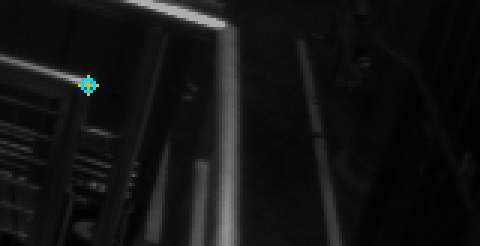
\includegraphics[width=\linewidth]{figures/method/mv-divergence-1}
  \end{minipage}\hfill
  \begin{minipage}[t]{0.485\textwidth}\centering
    \textbf{Four transitions later}\\[-0.15em]
    {\small MV to KLT gap: $0.86$ px}\par\smallskip
    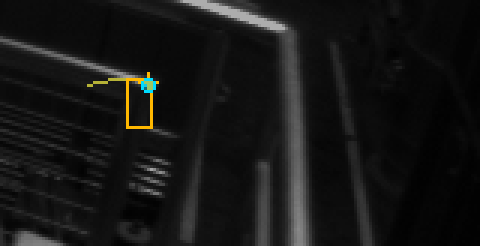
\includegraphics[width=\linewidth]{figures/method/mv-divergence-2}
  \end{minipage}

  \medskip
  \begin{minipage}[t]{0.485\textwidth}\centering
    \textbf{Nine transitions later}\\[-0.15em]
    {\small MV to KLT gap: $6.68$ px}\par\smallskip
    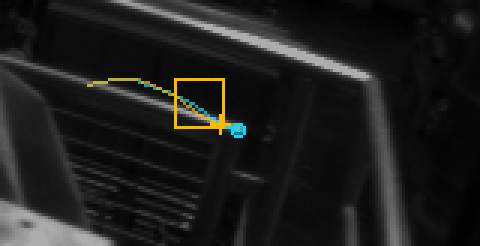
\includegraphics[width=\linewidth]{figures/method/mv-divergence-3}
  \end{minipage}\hfill
  \begin{minipage}[t]{0.485\textwidth}\centering
    \textbf{Fourteen transitions later}\\[-0.15em]
    {\small MV to KLT gap: $16.28$ px}\par\smallskip
    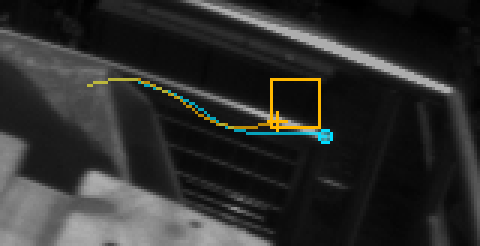
\includegraphics[width=\linewidth]{figures/method/mv-divergence-4}
  \end{minipage}
  \caption[Drift of a propagated codec sample from an image feature]{Failure of naive ID propagation on EMH01. Both diagnostic tracks
  start at the same selected image feature. Orange repeatedly applies the raw,
  unfiltered H.264 vector whose source block covers the preceding point; its
  rectangle shows that step's destination block support. Cyan is an OpenCV
  pyramidal KLT track computed
  after the experiment and retained only while its per-step forward-backward
  error is at most one pixel. It is diagnostic and is not consumed by the
  estimator. The nearest accepted compressed-stereo sample is $3.43$ pixels
  from the birth location and estimates a depth of $1.98$ metres. The trails
  show the full histories up to each displayed stage.}
  \label{fig:mv-feature-departure-example}
\end{figure}

Second, local inter-prediction support can disappear although the tracked image
structure remains visible. In \autoref{fig:mv-abrupt-stop-example}, raw motion
vectors remain present in the destination image at the first unsupported
transition, but none has a source block covering the previously propagated
point. The KLT diagnostic remains stable over the subsequent observations. The
trace alone does not identify whether this local absence
was caused by an intra-coded block, a partition change, or another encoder
decision. It nevertheless demonstrates why an absent vector cannot be equated
with an absent scene point.

\begin{figure}[htbp]
  \centering
  \begin{minipage}[t]{0.485\textwidth}\centering
    \textbf{Complete paths}\\[-0.15em]
    {\small codec path terminates; KLT continues}\par\smallskip
    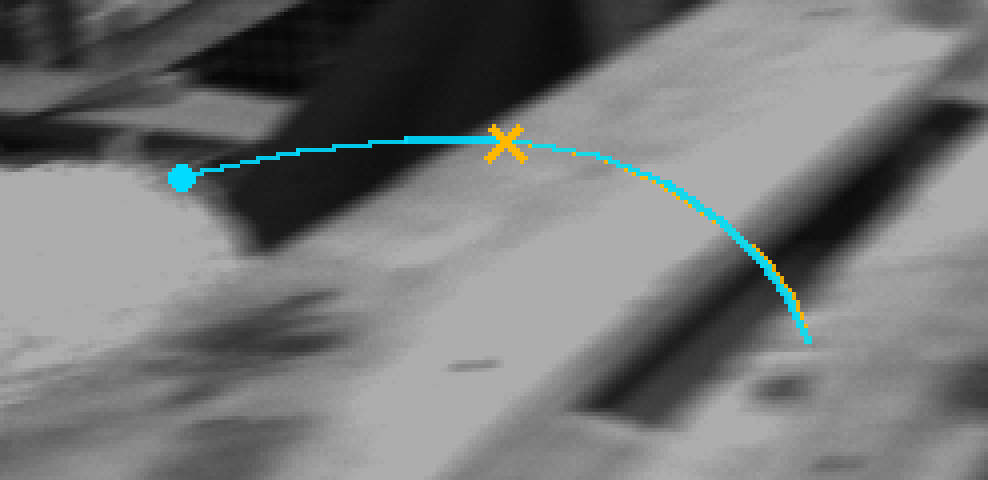
\includegraphics[width=\linewidth]{figures/method/mv-stop-combined}
  \end{minipage}\hfill
  \begin{minipage}[t]{0.485\textwidth}\centering
    \textbf{First unsupported transition}\\[-0.15em]
    {\small nearest raw-MV support is $6.0$ px away}\par\smallskip
    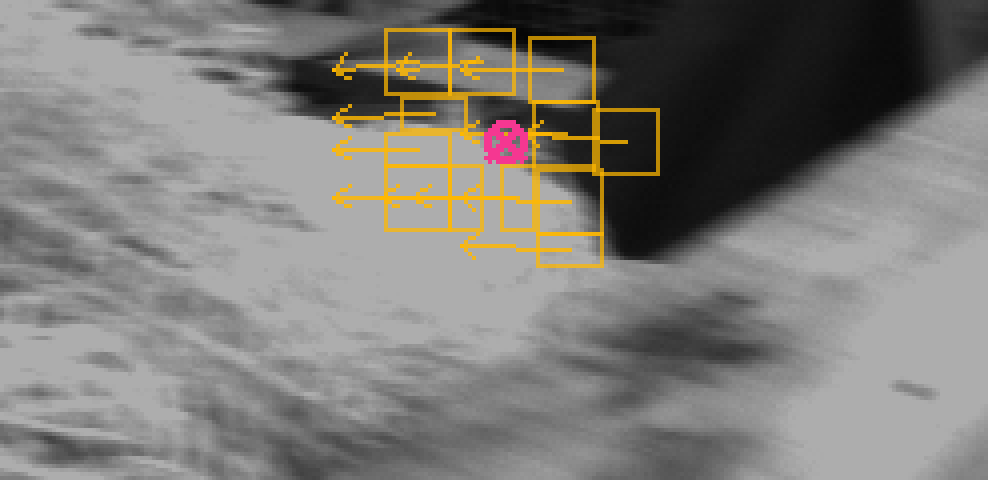
\includegraphics[width=\linewidth]{figures/method/mv-stop-neighborhood}
  \end{minipage}
  \caption[Abrupt local loss of codec support]{Abrupt local loss of codec support on EMH01. Orange and cyan have
  the same meanings as in \autoref{fig:mv-feature-departure-example}. The raw
  MV path follows the KLT diagnostic for six transitions and then terminates;
  the left panel places both complete paths on one image. The right panel shows
  a nearby subsample of the raw H.264 source supports and displacements used for
  the next transition. Other vectors are present locally, but none covers the
  propagated query marked in magenta. Decoded intensities are used only to
  construct this explanatory diagnostic.}
  \label{fig:mv-abrupt-stop-example}
\end{figure}

These two observations motivate reciprocal and geometric validation; neither
post-hoc KLT track is an additional pixel-domain gate in the method.

\section{Forward-Backward Consistency}

Tracking a point forward and then backward should return to its starting location when both estimates describe the same correspondence. Kalal et al. use this time-reversal principle to detect tracking failures from forward-backward error~\cite{kalal2010forwardbackward}. Zouein et al. apply a related directional-consistency test to tracks assembled from AV1 motion vectors~\cite{zouein2025leveraging}. Here the principle is adapted to H.264 block supports rather than image-tracked points.

Let $\mathbf{v}_f$ be a forward motion vector and let $\mathbf{v}_b$ be a vector from the reverse encoding, expressed in the same temporal direction. A candidate pair is retained only if its source and destination support rectangles overlap in both directions and
\begin{equation}
  \frac{\mathbf{v}_f^{\mathsf T}\mathbf{v}_b}
       {\lVert\mathbf{v}_f\rVert\lVert\mathbf{v}_b\rVert}
  \geq 0.98,
  \qquad
  \lVert\mathbf{v}_f-\mathbf{v}_b\rVert_2 \leq 1.5\ \text{px}.
\end{equation}
The minimum intersection-over-union of the corresponding source and destination supports must additionally be at least $0.15$. Two zero-displacement vectors are treated as directionally consistent. The validated support is the intersection that remains after translating both block supports into a common frame.

The retained hybrid policy uses reciprocal candidates for consensus estimation and continuation of established tracks. The larger best-direction pool may propose new tracks, but these remain provisional until a reciprocal continuation confirms a third observation. If only one encoding direction is available at an I-frame boundary, that direction is used as a fallback.

\begin{figure}[htbp]
  \centering
  \begin{minipage}[t]{0.315\textwidth}\centering
    \textbf{Forward: $64.78$ px}\par\smallskip
    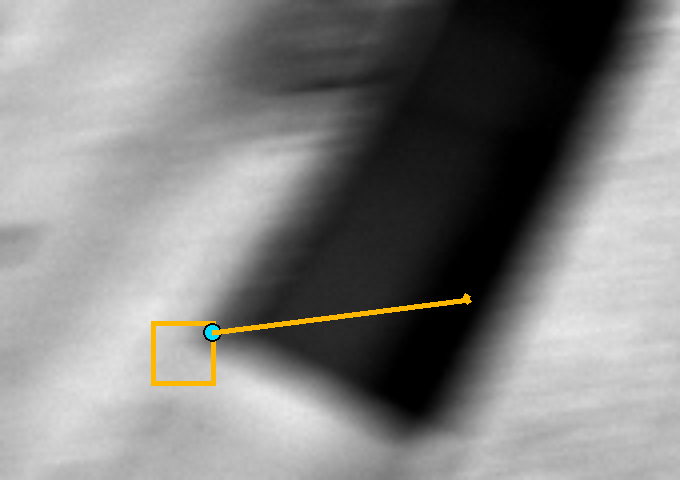
\includegraphics[width=\linewidth]{figures/method/reciprocal-accepted-1}
  \end{minipage}\hfill
  \begin{minipage}[t]{0.315\textwidth}\centering
    \textbf{Reverse: $65.03$ px}\par\smallskip
    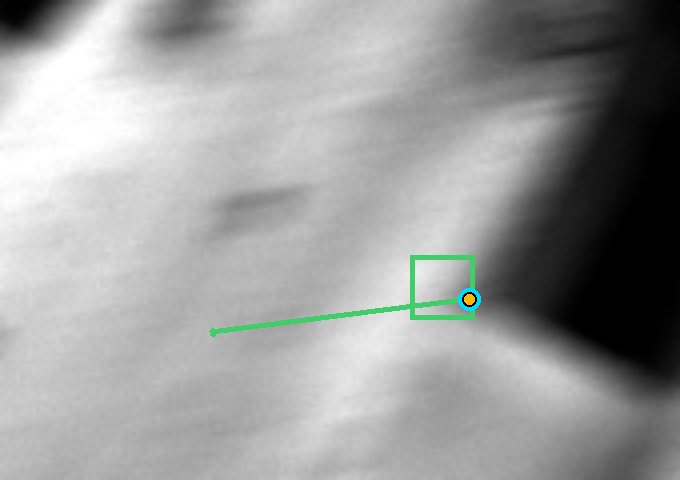
\includegraphics[width=\linewidth]{figures/method/reciprocal-accepted-2}
  \end{minipage}\hfill
  \begin{minipage}[t]{0.315\textwidth}\centering
    \textbf{Cycle closure: $0.25$ px}\par\smallskip
    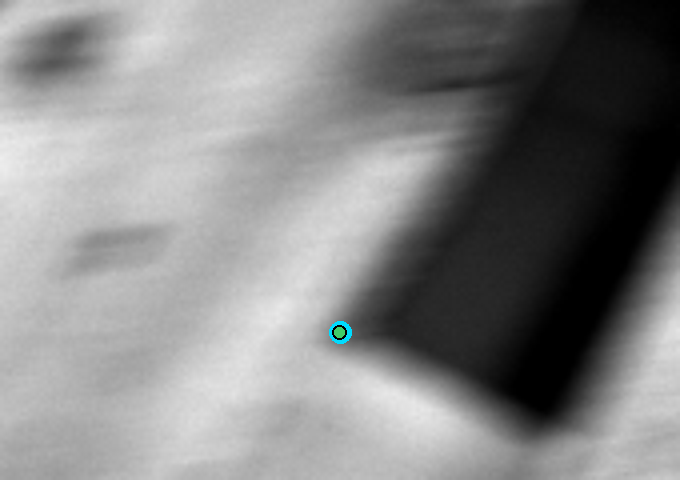
\includegraphics[width=\linewidth]{figures/method/reciprocal-accepted-3}
  \end{minipage}

  {\small cosine $1.000$, IoU $0.31$; codec/KLT endpoint difference $0.13$ px}
  \caption[Accepted reciprocal motion-vector correspondence]{An accepted large-displacement reciprocal match on EMH01. The cyan marker identifies a post-hoc KLT
  feature, the orange arrow is the forward codec motion, and the green arrow is
  the reverse-encoding motion. In the middle panel, the cyan KLT ring encloses
  the orange codec endpoint; in the final panel, the green return point lies
  within $0.25\,\mathrm{px}$ of the cyan source point. The KLT observation also
  passes its own forward-backward check with $0.06\,\mathrm{px}$ error. Image
  intensities are used only for this explanatory validation and are not inputs
  to reciprocal correspondence selection.}
  \label{fig:reciprocal-example}
\end{figure}

\section{Robust Association and Track Identity}

For a temporal candidate $(\mathbf{u}_{t-1},\mathbf{u}_t)$, compressed-domain
stereo supplies the distance $\lambda$ along the native anchor-camera bearing
at each endpoint. Let $\hat{\mathbf b}_A(\mathbf u)$ denote the corresponding
unit bearing. These ranges and bearings form a putative 3D-3D association
\begin{equation}
  \mathbf{a}_i = \lambda_{t-1,i}\,\hat{\mathbf b}_A(\mathbf{u}_{t-1,i}),
  \qquad
  \mathbf{b}_i = \lambda_{t,i}\,\hat{\mathbf b}_A(\mathbf{u}_{t,i}).
\end{equation}
Under the static-scene assumption, the inlier pairs share one rigid transformation. TEASER++ estimates this consensus with fixed scale and a $0.1\,\mathrm{m}$ noise bound~\cite{yang2020teaser}. Each candidate is then tested against the estimated transform. For points beyond $5\,\mathrm{m}$, a further $1.5\,\mathrm{px}$ reprojection gate rejects associations whose metric residual is small only because of weak depth geometry. If registration fails, no temporal association is accepted for that frame.

An accepted continuation inherits the existing landmark ID. A new association receives a provisional ID and is withheld from the backend until the following frame confirms it. TEASER++ therefore acts as an association filter; its frame-to-frame transform is not inserted as a camera-pose measurement.

\begin{figure}[htbp]
  \centering
  \begin{minipage}[t]{0.475\textwidth}\centering
    \textbf{Accepted: source}\\[-0.15em]
    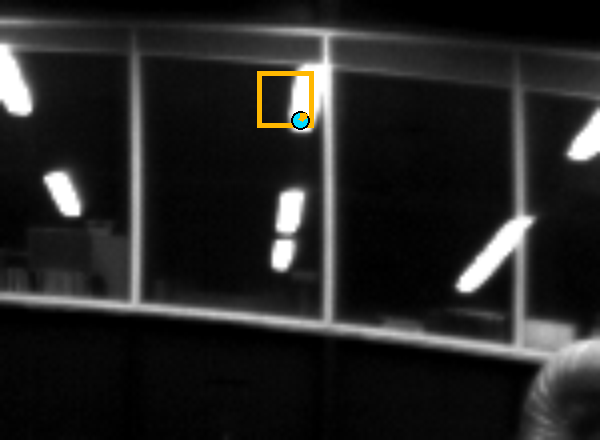
\includegraphics[width=\linewidth]{figures/method/teaser-accepted-source}
  \end{minipage}\hfill
  \begin{minipage}[t]{0.475\textwidth}\centering
    \textbf{Accepted: destination}\\[-0.15em]
    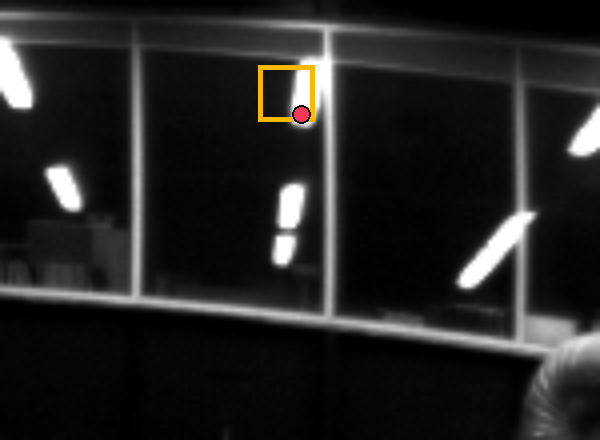
\includegraphics[width=\linewidth]{figures/method/teaser-accepted-destination}
  \end{minipage}\par\vspace{0.45em}
  \begin{minipage}[t]{0.475\textwidth}\centering
    \textbf{Rejected: source}\\[-0.15em]
    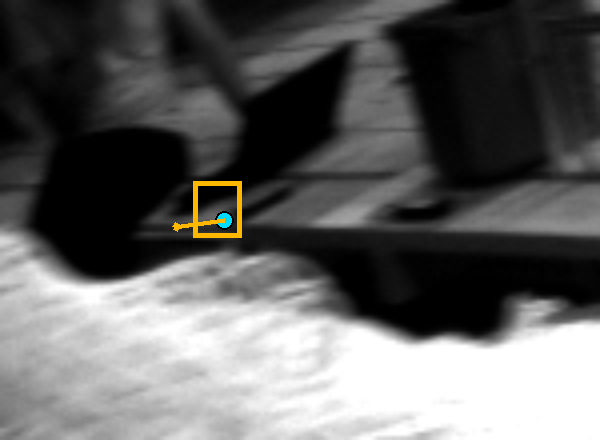
\includegraphics[width=\linewidth]{figures/method/teaser-rejected-source}
  \end{minipage}\hfill
  \begin{minipage}[t]{0.475\textwidth}\centering
    \textbf{Rejected: destination}\\[-0.15em]
    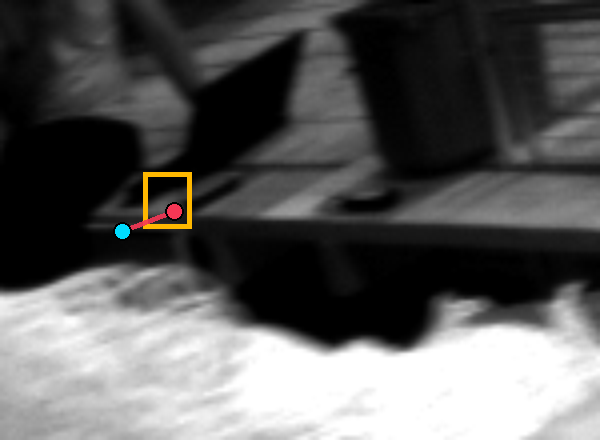
\includegraphics[width=\linewidth]{figures/method/teaser-rejected-destination}
  \end{minipage}
  \caption[Accepted and rejected robust-association candidates]{Individual robust-association decisions on EMH01. Orange outlines
  show the exact codec-block support, cyan marks a post-hoc KLT endpoint, and
  magenta marks the codec-motion endpoint. The accepted example has a
  $0.12\,\mathrm{px}$ endpoint difference. In the rejected example, the distinctly localized corner
  moves to the cyan position while the codec candidate ends
  $13.8\,\mathrm{px}$ away. Both KLT observations pass a one-pixel
  forward-backward check. KLT is used only to explain the decisions after
  estimation; TEASER++ receives the stereo 3D-3D candidates and no image data.}
  \label{fig:teaser-example}
\end{figure}

\section{Suppression of Indistinguishable Measurements}

Conventional feature frontends suppress nearby detections to avoid repeatedly representing the same local structure and to preserve spatially useful support~\cite{qin2018vins,kuhne2025lowlatency}. Codec blocks have no image-derived detector response on which to perform conventional non-maximum suppression. The proposed frontend instead suppresses measurements that cannot be distinguished at its available geometric resolution.

H.264 represents motion vectors at quarter-pixel precision and assigns each
vector to an extended prediction block. This finite spatial resolution motivates
treating sufficiently similar codec-derived observations as duplicate support.
Two accepted measurements are considered duplicates when their positions at both
temporal endpoints differ by at most $1.125\,\mathrm{px}$ in the $L_\infty$ norm
and their depth intervals overlap at both endpoints.

The interval model assigns a single-endpoint tolerance of $0.5625\,\mathrm{px}$,
half the selected suppression distance, giving a stereo-disparity tolerance of
$1.125\,\mathrm{px}$. It forms a disparity surrogate $f_xB/\lambda$ from the
triangulated camera range, perturbs it by the disparity tolerance, and maps the
limits back through the pinhole depth relation. A nonpositive lower disparity
limit gives an unbounded upper range limit. This is a pinhole approximation for
comparing depth support. The tolerances were selected in the parameter study;
quarter-pixel representation alone does not establish a bound on physical
correspondence error.

Candidates are processed in age order: established IDs are considered before new
births, and monotonically assigned IDs order older tracks first. The oldest
eligible representative is retained and suppresses younger indistinguishable
candidates. This favors continuity without inspecting image intensities.

\begin{figure}[htbp]
  \centering
  \begin{minipage}[t]{0.235\textwidth}\centering
    \textbf{Birth}\\[-0.15em]
    {\small $d_\infty=16.25$ px}\par\smallskip
    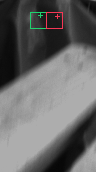
\includegraphics[width=\linewidth]{figures/method/suppression-retained-1}
  \end{minipage}\hfill
  \begin{minipage}[t]{0.235\textwidth}\centering
    \textbf{Age 4}\\[-0.15em]
    {\small $d_\infty=16.00$ px}\par\smallskip
    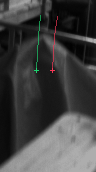
\includegraphics[width=\linewidth]{figures/method/suppression-retained-2}
  \end{minipage}\hfill
  \begin{minipage}[t]{0.235\textwidth}\centering
    \textbf{Age 7}\\[-0.15em]
    {\small $d_\infty=16.00$ px}\par\smallskip
    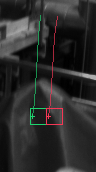
\includegraphics[width=\linewidth]{figures/method/suppression-retained-3}
  \end{minipage}\hfill
  \begin{minipage}[t]{0.235\textwidth}\centering
    \textbf{Age 10}\\[-0.15em]
    {\small $d_\infty=15.75$ px}\par\smallskip
    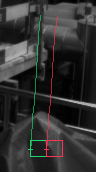
\includegraphics[width=\linewidth]{figures/method/suppression-retained-4}
  \end{minipage}
  \caption[Retention of nearby distinguishable tracks]{Two nearby but distinguishable EMH01 tracks over their complete
  ten-frame shared lifetime. Green and magenta identify the two retained IDs;
  the trails show their preceding image-plane observations. The centers are
  $16.25$ pixels apart at birth and remain between $15.75$ and $16.25$ pixels
  apart while moving approximately $135$ pixels through the image. Both IDs
  therefore survive age-prioritized suppression. This illustrates that the
  method does not enforce generic spatial sparsity: it removes only pairs that
  meet the $1.125$ pixel and depth-overlap criteria. Rectangles show the exact
  H.264 block dimensions rather than enlarged display regions.}
  \label{fig:suppression-example}
\end{figure}

\begin{figure}[htbp]
  \centering
  \begin{minipage}[t]{0.235\textwidth}\centering
    \textbf{Birth}\\[-0.15em]
    {\small $d_\infty=4.50$ px}\par\smallskip
    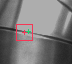
\includegraphics[width=\linewidth]{figures/method/suppression-merged-1}
  \end{minipage}\hfill
  \begin{minipage}[t]{0.235\textwidth}\centering
    \textbf{Age 2}\\[-0.15em]
    {\small $d_\infty=4.25$ px}\par\smallskip
    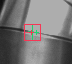
\includegraphics[width=\linewidth]{figures/method/suppression-merged-2}
  \end{minipage}\hfill
  \begin{minipage}[t]{0.235\textwidth}\centering
    \textbf{Age 3}\\[-0.15em]
    {\small $d_\infty=1.75$ px}\par\smallskip
    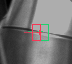
\includegraphics[width=\linewidth]{figures/method/suppression-merged-3}
  \end{minipage}\hfill
  \begin{minipage}[t]{0.235\textwidth}\centering
    \textbf{Age 4}\\[-0.15em]
    {\small younger ID suppressed}\par\smallskip
    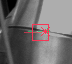
\includegraphics[width=\linewidth]{figures/method/suppression-merged-4}
  \end{minipage}
  \caption[Suppression of an indistinguishable younger track]{An age-prioritized suppression event recorded at the original
  $2.25$-pixel component-ablation setting on EMH01. The two
  accepted tracks are distinguishable at birth, approach one another, and end
  $1.75$ pixels apart for two consecutive observations. The older green ID is
  retained; the crossed magenta ID is omitted once the endpoint and
  depth-overlap tests both identify the measurements as indistinguishable. The
  selected PVO setting applies the same rule with a $1.125$-pixel bound.}
  \label{fig:suppression-merged-example}
\end{figure}

\section{Rigid-Flow Bundle Adjustment}

\subsection{Observation Model}

Conventional bundle adjustment treats an image coordinate
$\mathbf{u}_{j,t}^{c}$ as a noisy observation of a projected landmark,
\begin{equation}
  \mathbf{e}_{j,t}^{c}
  = \widehat{\mathbf{u}}_{j,t}^{c}-\mathbf{u}_{j,t}^{c},
  \qquad
  \widehat{\mathbf{u}}_{j,t}^{c}
  = \pi_c\!\left(\mathbf{T}_{WC_t}^{-1}\mathbf{p}_j^W\right).
\end{equation}
A codec block instead supplies a displacement over an extended prediction
region, without identifying a particular scene point within that region.
For an anchor-camera track propagated from an initial sample, the stored
coordinate after several accepted displacements is
\begin{equation}
  \mathbf{u}_{j,t}^{c}
  = \mathbf{u}_{j,0}^{c}+\sum_{k=1}^{t}\mathbf{m}_{j,k}^{c}.
\end{equation}
Absolute reprojection assigns each resulting coordinate a point-observation
residual. An earlier block-selection or displacement error can therefore affect
several later residuals. A fixed per-observation variance does not represent
this temporal correlation; it does not, however, imply that the coordinates
are assumed noise-free.

The evaluated alternative replaces eligible absolute factors with displacement
factors. Let $s$ be the predecessor timestamp explicitly recorded for
observation $(j,t,c)$. In the evaluated frontend this is the preceding processed
frame when the same ID has a stored observation in that camera. It is not
reassigned to an older retained keyframe if that predecessor is removed.
The shared landmark and two poses predict
\begin{equation}
  \Delta\widehat{\mathbf{u}}_{j,t}^{c}
  = \widehat{\mathbf{u}}_{j,t}^{c}
    -\widehat{\mathbf{u}}_{j,s}^{c},
\end{equation}
while the recorded measurement is
\begin{equation}
  \mathbf{m}_{j,t}^{c}
  = \mathbf{u}_{j,t}^{c}-\mathbf{u}_{j,s}^{c}.
\end{equation}
The rigid-flow residual is their difference,
\begin{equation}
  \mathbf{r}_{j,t}^{c}
  = \Delta\widehat{\mathbf{u}}_{j,t}^{c}-\mathbf{m}_{j,t}^{c}.
  \label{eq:rigid-flow-residual}
\end{equation}
Here \emph{rigid flow} means the image displacement predicted by reprojecting
one static landmark through two camera poses. It is not an additional measured
3D motion. The factor constrains a difference of projections without attaching
either endpoint to an absolute codec sample. Other factors still provide
absolute constraints, as detailed below. Shared poses and one persistent
landmark state couple the available temporal factors across a track.
This construction changes the observation model; it neither makes codec
correspondences exact nor removes the possibility of accumulated pose drift.

In the evaluated implementation, the frontend records the predecessor and
endpoint difference separately for each camera whenever both same-ID samples
are present. Anchor-camera samples are propagated using the selected temporal
motion vector. Stereo-camera samples are obtained from codec-stereo
correspondences and expressed in native stereo-camera pixels. Their stored
endpoint difference supplies $\mathbf{m}_{j,t}^{S}$; it is not a separately
queried temporal vector from the stereo camera. When both camera factors are
available, they share a landmark and pose pair but use their respective
calibrated projections. Missing flow metadata, including for some backfilled
birth observations, leaves an absolute observation instead.
\autoref{fig:absolute-versus-rigid-flow} illustrates the two observation models.

\begin{figure}[p]
  \centering
  \resizebox{!}{0.74\textheight}{%
  \begin{tikzpicture}[
      plane/.style={draw=TUMDarkGray,fill=TUMBlue!5,line width=0.45pt},
      sphere/.style={draw=TUMDarkGray!45,densely dotted},
      ray/.style={draw=TUMDarkGray!65,densely dotted},
      measured/.style={->,very thick,color=TUMAccentOrange},
      predicted/.style={->,very thick,color=TUMBlue},
      residual/.style={->,thick,color=red!75!black},
      artificial/.style={rectangle,draw=TUMAccentOrange,
        fill=TUMAccentOrange,inner sep=2.2pt}]
    \begin{scope}
      \node[font=\bfseries] at (2.5,5.05) {Absolute reprojection};
      \coordinate (P) at (2.5,2.70);
      \draw[sphere] (P) circle[radius=1.72];
      \fill[black] (P) circle[radius=2.3pt];
      \node[font=\small,above right] at (P) {$\mathbf p^W$};

      \begin{scope}[shift={(1.28,1.48)},rotate=-44]
        \path[plane] (-0.70,-0.22) -- (0.64,-0.15) --
          (0.70,0.22) -- (-0.64,0.15) -- cycle;
        \coordinate (p0) at (-0.12,0.00);
        \node[circle,fill=TUMBlue,inner sep=2.2pt] at (p0) {};
        \coordinate (a0) at (0.18,0.07);
        \node[artificial] at (a0) {};
      \end{scope}
      \begin{scope}[shift={(2.5,4.35)}]
        \path[plane] (-0.70,-0.20) -- (0.64,-0.13) --
          (0.70,0.20) -- (-0.64,0.13) -- cycle;
        \coordinate (p1) at (-0.16,0.00);
        \node[circle,fill=TUMBlue,inner sep=2.2pt] at (p1) {};
        \coordinate (a1) at (0.23,0.06);
        \node[artificial] at (a1) {};
      \end{scope}
      \begin{scope}[shift={(3.72,1.48)},rotate=44]
        \path[plane] (-0.70,-0.22) -- (0.64,-0.15) --
          (0.70,0.22) -- (-0.64,0.15) -- cycle;
        \coordinate (p2) at (-0.10,0.00);
        \node[circle,fill=TUMBlue,inner sep=2.2pt] at (p2) {};
        \coordinate (a2) at (0.28,0.07);
        \node[artificial] at (a2) {};
      \end{scope}
      \draw[ray] (P) -- (p0);
      \draw[ray] (P) -- (p1);
      \draw[ray] (P) -- (p2);
      \draw[measured] (a0) -- (a1);
      \draw[measured] (a1) -- (a2);
      \draw[residual] (a0) -- node[below,font=\scriptsize,inner sep=0.4444em] {$\mathbf e_{t-1}$} (p0);
      \draw[residual] (a1) -- node[above,font=\scriptsize,inner sep=0.4444em] {$\mathbf e_t$} (p1);
      \draw[residual] (a2) -- node[right,xshift=6pt,yshift=-2.3333pt,font=\scriptsize] {$\mathbf e_{t+1}$} (p2);
      \node[font=\scriptsize] at (0.62,0.72) {$\Pi_{t-1}$};
      \node[font=\scriptsize] at (1.62,4.35) {$\Pi_t$};
      \node[font=\scriptsize] at (4.38,0.72) {$\Pi_{t+1}$};
    \end{scope}

    \begin{scope}[yshift=-5.7cm]
      \node[font=\bfseries] at (2.5,5.05) {Rigid-flow reprojection};
      \coordinate (Q) at (2.5,2.70);
      \draw[sphere] (Q) circle[radius=1.72];
      \fill[black] (Q) circle[radius=2.3pt];
      \node[font=\small,above right] at (Q) {$\mathbf p^W$};

      \begin{scope}[shift={(1.28,1.48)},rotate=-44]
        \path[plane] (-0.70,-0.22) -- (0.64,-0.15) --
          (0.70,0.22) -- (-0.64,0.15) -- cycle;
        \coordinate (q0) at (-0.12,0.00);
        \node[circle,fill=TUMBlue,inner sep=2.4pt] at (q0) {};
      \end{scope}
      \begin{scope}[shift={(2.5,4.35)}]
        \path[plane] (-0.70,-0.20) -- (0.64,-0.13) --
          (0.70,0.20) -- (-0.64,0.13) -- cycle;
        \coordinate (q1) at (-0.16,0.00);
        \node[circle,fill=green!60!black,inner sep=2.4pt] at (q1) {};
        \coordinate (m1) at (0.12,-0.12);
      \end{scope}
      \begin{scope}[shift={(3.72,1.48)},rotate=44]
        \path[plane] (-0.70,-0.22) -- (0.64,-0.15) --
          (0.70,0.22) -- (-0.64,0.15) -- cycle;
        \coordinate (q2) at (-0.10,0.00);
        \node[circle,fill=violet!85!black,inner sep=2.4pt] at (q2) {};
        \coordinate (m2) at (0.18,-0.13);
      \end{scope}
      \draw[ray] (Q) -- (q0);
      \draw[ray] (Q) -- (q1);
      \draw[ray] (Q) -- (q2);
      \draw[predicted] (q0) -- (q1);
      \draw[predicted] (q1) -- (q2);
      \draw[measured] (q0) -- (m1);
      \draw[measured] (q1) -- (m2);
      \draw[residual] (m1) -- node[right,font=\scriptsize,inner sep=0.4444em] {$\mathbf r_t$} (q1);
      \draw[residual] (m2) -- node[right,xshift=6pt,yshift=-2.3333pt,font=\scriptsize] {$\mathbf r_{t+1}$} (q2);
      \node[font=\scriptsize] at (0.62,0.72) {$\Pi_{t-1}$};
      \node[font=\scriptsize] at (1.62,4.35) {$\Pi_t$};
      \node[font=\scriptsize] at (4.38,0.72) {$\Pi_{t+1}$};
    \end{scope}
  \end{tikzpicture}}
  \caption[Absolute reprojection and rigid-flow residuals]{Schematic comparison for one static landmark observed at
  three consecutive times. Top: absolute factors compare propagated codec samples
  (orange squares) with individual projections. Bottom: rigid-flow factors compare
  predicted displacement (blue) with recorded displacement (orange).
  Red arrows follow the predicted-minus-measured residual convention.
  Connections between the drawn image planes indicate temporal coupling;
  displacement subtraction is performed in image-pixel coordinates, not in
  the page-space geometry of this illustration.}
  \label{fig:absolute-versus-rigid-flow}
\end{figure}

\subsection{Shared State and Jacobian Assembly}

The implementation stores each landmark in its host camera, using two bearing
parameters and inverse distance,
$\boldsymbol{\ell}_j=(\alpha_j,\beta_j,\rho_j)^{\mathsf T}$.
The unit bearing $\mathbf b(\alpha_j,\beta_j)$ and $\rho_j$ form the homogeneous
point
\begin{equation}
  \overline{\mathbf p}_{h,j}(\boldsymbol{\ell}_j)
    = \begin{bmatrix}\mathbf b(\alpha_j,\beta_j)\\ \rho_j\end{bmatrix},
  \qquad
  \widehat{\mathbf u}_{j,k}^{c}
    = \pi_c\!\left(\mathbf T_{kh}
             \overline{\mathbf p}_{h,j}(\boldsymbol{\ell}_j)\right).
\end{equation}
Here $\mathbf T_{kh}$ maps the landmark host camera to camera $c$ at time $k$;
it combines the host and target body poses with the fixed camera extrinsics.
Both projections use the same $\boldsymbol{\ell}_j$, rather than independently
parameterized points at $s$ and $t$.

The two predictions are functions of one joint optimization state containing
the host pose, predecessor pose, current pose, and shared landmark. Therefore
\begin{equation}
  \frac{\partial\mathbf r}{\partial\mathbf x}
    = \frac{\partial\widehat{\mathbf u}_{j,t}^{c}}{\partial\mathbf x}
      -\frac{\partial\widehat{\mathbf u}_{j,s}^{c}}{\partial\mathbf x}.
\end{equation}
This subtraction requires identical state columns, with zeros for variables
absent from a projection. It does not identify the predecessor and current
poses as one variable.

Basalt first differentiates a projection with respect to its local
host-to-target pose perturbation and the landmark
parameters~\cite{usenko2020visual}. Denote these derivatives by
$\mathbf D_k\in\mathbb R^{2\times6}$ and
$\mathbf L_k\in\mathbb R^{2\times3}$.
Let $\mathbf A_{kh}$ and $\mathbf A_{kk}$ map the absolute host and target
body-pose perturbations into that local relative-pose perturbation. For
distinct host, predecessor, and current poses, the residual blocks are
\begin{equation}
  \begin{aligned}
    \mathbf J_h &= \mathbf D_t\mathbf A_{th}
                  -\mathbf D_s\mathbf A_{sh},&
    \mathbf J_s &= -\mathbf D_s\mathbf A_{ss},\\
    \mathbf J_t &= \mathbf D_t\mathbf A_{tt},&
    \mathbf J_{\ell} &= \mathbf L_t-\mathbf L_s.
  \end{aligned}
  \label{eq:rigid-flow-block-jacobians}
\end{equation}
Current and predecessor pose terms are placed in separate columns.
Subtraction within one block occurs for the shared landmark and, after the
chain rule, the shared host pose. If a host and target use the same body pose,
their contributions accumulate in the same block. When both timestamp and
camera are identical, the relative transform is identity and its pose
derivatives are zero.

The backend retains Basalt's pose-linearization convention: the
$\mathbf A$ maps are evaluated at stored pose linearization points, while the
projection transform is updated from the current estimates when those points
are held fixed. The local projection derivatives are evaluated using that
transform and the current landmark. Thus the block assembly above also applies
when marginalization has fixed the pose reference points; it does not imply
that every derivative is recomputed at the latest pose estimate.

\subsection{Factor Allocation and Weighting}

Both cameras are enabled for rigid-flow factors in the evaluated configuration.
A current observation receives a flow factor only if it is not the landmark's
host-camera observation, its finite flow measurement identifies an earlier
observation of the same ID in the same camera, and both poses are in the active
state ordering. Otherwise, an active observation receives an absolute factor.
The allocation is exclusive: one observation is never represented by both
factors in the same joint problem. If a selected flow factor has an invalid
projection at either endpoint, it contributes no residual at that
linearization; this projection failure does not trigger an absolute fallback.
The nonlinear objective and the linear system implement the same residual
definition and structural selection rule in separate routines.

For joint-window visual factors, the Huber weight is computed from the
two-dimensional residual norm in pixels before scaling by the observation
standard deviation. Holding this weight fixed for each linearization gives
the weighted residual and Jacobian rows used in the linear system:
\begin{equation}
  w_H =
  \begin{cases}
    1, & \|\mathbf r\|\leq\delta,\\
    \delta/\|\mathbf r\|, & \|\mathbf r\|>\delta,
  \end{cases}
  \qquad
  \widetilde{\mathbf r}=\frac{\sqrt{w_H}}{\sigma}\mathbf r,
  \qquad
  \widetilde{\mathbf J}=\frac{\sqrt{w_H}}{\sigma}\mathbf J .
\end{equation}
The selected settings are $\sigma=4$ pixels and $\delta=0.5$ pixels. Absolute
and displacement factors use this same scalar weighting; the model does not
introduce a separate flow covariance or temporal error-correlation matrix.
The residual ablation changes only this backend factor allocation in joint
optimization and marginalization,
holding the frontend and other backend settings fixed.

\subsection{Optimization and Marginalization}

After the incoming pose and its observations have been inserted, a pose-only
initialization step uses absolute reprojection of already connected landmarks.
It performs two Gauss--Newton updates with small damping; its normal equations
use unweighted valid projection residuals. The robust weighting described above
applies to the subsequent joint optimization and marginalization, not to these
initialization updates. All of these coordinates come from codec metadata and
calibrated geometry, without consulting image intensities.

A keyframe is requested when the fraction of currently observed anchor-camera
IDs connected to landmarks falls below $0.8$, provided more than one frame has elapsed since
the previous keyframe. New landmarks are triangulated from multi-camera or
multi-frame observations. Joint optimization uses absolute square-root QR
linearization to eliminate landmark increments, then solves the damped reduced
pose system. This is one coupled window problem, not an independent pose fit
for each flow measurement.

After optimization, old non-keyframe poses and their observations are removed
before the marginalization system is constructed. The most recent pose is
retained, so a preceding non-keyframe can still participate in the next joint
solve before its removal. After marginalization, the retained state contains
at most seven keyframes plus the current pose if it is not already a keyframe;
the joint solve can temporarily contain additional poses. The configured
three-state limit belongs to the inertial estimator and is inactive here.

Square-root marginalization forms a prior from the existing prior and selected
landmarks hosted by departing keyframes or classified as lost. Those
landmarks use the same factor-allocation rule on the observations and poses
that remain at this stage. Surviving eligible flow factors can therefore enter
the prior, but the procedure does not preserve every historical flow factor:
removal of a predecessor can make an observation use absolute reprojection,
and there is no replacement flow edge to another retained frame. The
separately explored pre-marginalization outlier-removal step and second
optimization pass are disabled in the evaluated method.

\section{Integration and Frame Processing}

The retained hybrid policy separates continuation from birth. Established IDs
may continue only through reciprocal forward-backward candidates. The larger
union of forward and inverted-reverse candidates may propose births, allowing
coverage where one direction is preferable, but a new ID remains provisional
until a reciprocal observation confirms it in the following frame. The frontend
therefore buffers two frames before publishing them to the backend. Once
confirmed, the withheld observations for the first two frames and the third
observation are emitted with one ID. A provisional track that fails confirmation
is discarded. At shutdown, buffered frames are flushed in timestamp order, but
unconfirmed births are not promoted.

The per-frame procedure is summarized below.

\begin{center}
\begin{minipage}{0.97\textwidth}
\hrule
\vspace{0.35em}
\textbf{Algorithm 1:} Pixel-free processing of frame $t$.
\vspace{0.35em}
\hrule
\vspace{0.25em}
\begin{tabular}{@{}r@{\hspace{0.8em}}p{0.91\linewidth}@{}}
  1 & \textbf{Input:} temporal and stereo MVs, calibration, masks, tracks, and backend state. \\
  2 & \textbf{Output:} confirmed observations with IDs and updated state. \\
  3 & Normalize MVs; apply source, mask, bounds, and median checks. \\
  4 & Form best-direction birth and reciprocal continuation pools. \\
  5 & Obtain stereo at both endpoints; fit fixed-scale TEASER++ to spatially subsampled 3D pairs. \\
  6 & Retain candidates passing stereo, rigid-consensus, and far-depth gates. \\
  7 & \textbf{for} active IDs $j$, oldest first, \textbf{do} \\
  8 & \quad Select the reciprocal successor with minimum 3D residual. \\
  9 & \quad Continue $j$ and record both camera displacements if suppression retains it. \\
 10 & \textbf{end} \\
 11 & Allocate provisional IDs from unused birth candidates surviving suppression. \\
 12 & Confirm provisional IDs after a reciprocal third observation. \\
 13 & Release confirmed observations after the two-frame delay. \\
 14 & For released frames, optimize the current pose and update keyframes and landmarks. \\
 15 & Optimize the active window and marginalize as required. \\
\end{tabular}
\vspace{0.25em}
\hrule
\end{minipage}
\end{center}

% !TeX root = ../main.tex

\chapter{Experimental Methodology}\label{chapter:experimental-methodology}

\section{Research Design}

The evaluation separates three forms of evidence. First, Pixelless VO (PVO) is
compared with a stationary baseline and two pixel-refined reference
configurations. Second, a component ablation holds the stereo frontend,
TEASER++ registration, rigid-flow residual, backend settings, and encoded input
fixed while enabling reciprocal motion-vector agreement and spatial suppression
individually and jointly. Third, offline diagnostics measure track persistence,
stereo support, image-structure coincidence, and the conditions associated with
large local error. The latter measurements explain the operating envelope but
are not inputs to the estimator.

All trajectory tables use full-sequence runs. The reported PVO trajectory uses
the operating point selected by the bounded parameter study described below;
short smoke tests, abandoned variants, and results from non-equivalent
diagnostic builds are excluded. Every reported configuration completed
all eleven sequences; a failed or incomplete run would be reported as missing
rather than replaced by a numeric value.

\section{Dataset}

Experiments use all eleven sequences of the EuRoC MAV dataset, an established
benchmark for visual odometry and SLAM, with its supplied stereo calibration
and ground truth~\cite{burri2016euroc}. The evaluated sequence
aliases, difficulty labels, and frame counts are listed in
\autoref{tab:euroc-evaluation-set}.

Other relevant benchmarks include TUM-VI~\cite{schubert2018vidataset} and the
Monado SLAM Dataset~\cite{deMayoCremersPireMSD}. The choice of EuRoC for the
final evaluation is primarily motivated by two practical requirements of the
present construction: broad usable coverage after stereo rectification and
the availability of depth at both endpoints of temporal correspondences.
The encoder-stereo stage adapted from Passthrough+ operates on rectified
views~\cite{chaurasia2020passthrough} and can recover depth only where both
cameras observe the scene. EuRoC's nearly parallel camera pair is well suited
to the common pinhole projection used here. TUM-VI's wide-angle images and
Monado's varied headset camera arrangements require more adaptation to retain
useful image support in that projection.

A reanalysis of the archived pilot calibrations quantifies the coverage
restriction. Of the calibrated, safe-radius-valid native left-image pixel
centres, \SI{97.0}{\percent} project inside the chosen rectified image on
EuRoC, compared with \SI{51.5}{\percent} on TUM-VI and
\SIrange{58.4}{78.7}{\percent} across the tested Monado camera pairs.
These fractions describe native-to-rectified image coverage. Temporal
candidates outside this domain cannot obtain stereo depth through the
implemented lookup, irrespective of the availability of temporal motion
vectors. Raw image resolution alone does not explain the dataset choice:
the Monado Index trials used $960\times960$ images, exceeding EuRoC's
$752\times480$ resolution.

The preliminary runs also show substantially less usable stereo-temporal
support. After the stereo geometric checks, approximately
\SIrange{74.1}{74.8}{\percent} of temporal candidates had depth at both
endpoints on the two easy Machine Hall pilot sequences, compared with about
\SI{43}{\percent} on TUM-VI room2 and room5 and
\SIrange{6.4}{17.3}{\percent} on the four tested Monado sequences. Such
missing depth prevents candidates from forming the 3D--3D correspondences
required by this frontend. These coverage and support limitations motivated
concentrating the final feasibility evaluation on EuRoC; further adaptation
of rectification and codec-domain stereo to the other camera configurations
lies outside its scope. The pilot observations concern the tested
configurations and do not establish a general limitation of those datasets
or of Passthrough+.

\begin{table}[htbp]
  \centering
  \caption[EuRoC evaluation sequences]{EuRoC sequences used by the full-sequence evaluation.}
  \label{tab:euroc-evaluation-set}
  \begin{tabular}{@{}lllrl@{}}
    \toprule
    Alias & EuRoC sequence & Difficulty & Frames & Camera rate \\
    \midrule
    EMH01 & MH\_01\_easy      & Easy      & 3682 & \SI{20}{\hertz} \\
    EMH02 & MH\_02\_easy      & Easy      & 3040 & \SI{20}{\hertz} \\
    EMH03 & MH\_03\_medium    & Medium    & 2700 & \SI{20}{\hertz} \\
    EMH04 & MH\_04\_difficult & Difficult & 2032 & \SI{20}{\hertz} \\
    EMH05 & MH\_05\_difficult & Difficult & 2273 & \SI{20}{\hertz} \\
    EV101 & V1\_01\_easy      & Easy      & 2912 & \SI{20}{\hertz} \\
    EV102 & V1\_02\_medium    & Medium    & 1710 & \SI{20}{\hertz} \\
    EV103 & V1\_03\_difficult & Difficult & 2149 & \SI{20}{\hertz} \\
    EV201 & V2\_01\_easy      & Easy      & 2280 & \SI{20}{\hertz} \\
    EV202 & V2\_02\_medium    & Medium    & 2348 & \SI{20}{\hertz} \\
    EV203 & V2\_03\_difficult & Difficult & 1921 & \SI{20}{\hertz} \\
    \bottomrule
  \end{tabular}
\end{table}

Encoded stereo and reverse-temporal streams are aligned by timestamp rather than
row number. Where preprocessing produced a one-frame terminal mismatch, the
unpaired terminal timestamp was omitted from the longer stream; no timestamp
shift or hard common-length truncation was applied.

\section{Compared Configurations}

\begin{description}
  \item[Stationary] Baseline that repeats the initial pose.
  \item[TEASER++ only] Motion-vector method with TEASER++ and rigid-flow optimization, without forward-backward agreement or non-maximum suppression.
  \item[Forward-backward] TEASER++-only method with reciprocal agreement and delayed confirmation.
  \item[NMS] TEASER++-only method with age-prioritized suppression of indistinguishable measurements.
  \item[Pixelless VO (PVO)] Proposed codec-only method using reciprocal checks,
    age-prioritized suppression, TEASER++ registration, and rigid-flow
    optimization.
  \item[VOCA MV-first] Frozen reference~\cite{hilscher2026voca}. Codec motion vectors initialize the first
    KLT pass; tracks not recovered in that pass are retried with unseeded optical
    flow.
  \item[VOCA OF-first] Frozen reference. Ordinary KLT optical flow is attempted
    first; lost tracks are retried with motion-vector initialization.
\end{description}

The stationary baseline and the TEASER++-only estimator are distinct
configurations. The VOCA MV-first and OF-first values are taken from their
frozen full-sequence evaluations; diagnostic runs are not substituted for those
trajectories.

\section{Encoding and Preprocessing Configuration}

All streams are encoded with FFmpeg 4.4.2 and \texttt{libx264} in the H.264
High profile with \texttt{yuv420p} output. The enabled partitions are
\texttt{p8x8}, \texttt{p4x4}, and \texttt{i8x8}. For the temporal streams,
the remaining x264 options
are \texttt{keyint=1000}, \texttt{me=umh}, \texttt{merange=64},
\texttt{subme=6}, \texttt{bframes=0}, and \texttt{ref=1}. The encoder uses
two-pass rate control at
\SI{500}{\kilo\bit\per\second}. Images listed by each camera's timestamp CSV
are supplied through FFmpeg's concat demuxer and encoded at 30 frames per
second. This encoded rate controls the container timestamps but does not replace
the EuRoC nanosecond timestamps used by the estimator and evaluation. H.264
fractional motion is preserved using each vector's reported numerator and scale;
no integer rounding is applied.

For every camera, a reverse-temporal stream is made by reversing the same ordered
image list and applying the identical temporal encoder settings. The extracted
reverse vectors are subsequently inverted and remapped to the corresponding
forward-time EuRoC timestamps. Forward and reverse files are required to contain
the same number of frames as the synchronized dataset metadata.
The single-reference configuration limits prediction dependencies within each
encoded stream, but two-pass rate control and reversal of complete sequences
make this preparation offline. No end-to-end real-time claim follows from
\texttt{ref=1} or the absence of B-frames.

Stereo preprocessing first applies the calibration-dependent common projection
described in \autoref{chapter:method}. It then encodes twelve independent
full-frame stereo streams: disparity shifts 0, 8, and 32 pixels crossed with
grid phases $(0,0)$, $(4,0)$, $(0,4)$, and $(4,4)$ pixels. Each source stereo
pair is expanded to an I-P-P triple and encoded at 90 frames per second with
CRF 23. The temporal motion-search and partition settings are retained, while
\texttt{keyint=3}, \texttt{min-keyint=3}, \texttt{scenecut=0},
\texttt{bframes=0}, and \texttt{ref=1} enforce independent triples. The I-P-P
reference structure and shift strategy are adapted from Passthrough+~\cite{chaurasia2020passthrough}; the mosaic layout,
hardware encoder, and subsequent depth processing are not reproduced.

Preprocessing verifies the frame type of every triple, equal timestamp order for
the stereo pair, exact forward/reverse frame counts, the presence of all twelve
shift combinations, and non-empty validity masks. The full command templates are
given in \autoref{appendix:reproducibility}; the immutable evaluation manifest
also records the exact FFmpeg version and hashes of the configurations used.

\section{Estimator Configuration}

All evaluated estimators are visual-only: IMU input and real-time enforcement are
disabled. The proposed method uses a calibrated anchor/stereo pair, an absolute square-root QR
linearization, square-root marginalization, at most seven retained keyframes
plus the current pose after marginalization, and a keyframe connection-ratio threshold of 0.8. With the
minimum-frames-after-keyframe parameter set to 1 and a strict counter test, a
new keyframe can be requested only after more than one frame has elapsed.
The Levenberg--Marquardt iteration-limit parameter is set to 7, with an
initial damping value of $10^{-4}$. Joint-window visual factors use an observation
standard deviation of 4 pixels and a Huber threshold of 0.5 pixels, applied to
the residual norm before normalization. Rigid-flow factors are enabled for
eligible observations in both the anchor and stereo cameras; host and
ineligible observations retain absolute factors. Standard marginalization and
lost-landmark removal
remain active; the additional pre-marginalization filtering and second
optimization pass evaluated in earlier experiments remain disabled.

\autoref{tab:frozen-frontend-parameters} lists the selected PVO frontend thresholds. Before
TEASER++ estimation, at most one stereo-temporal pair per
$40\times40$-pixel cell is retained using the stereo matching cost. TEASER++
uses fixed scale, a \SI{0.1}{\metre} noise bound, GNC-TLS rotation estimation,
and heuristic maximum-clique inlier selection~\cite{yang2020teaser}. PVO enables the
hybrid reciprocal-confirmation policy and indistinguishable-measurement
suppression. At the original operating point, the four component-ablation
configurations differ only in these two switches; their joint use is labelled
``Joint frontend.'' PVO uses the same complete method with selected frontend
thresholds and backend weights.

\begin{table}[htbp]
  \centering
  \caption[Selected PVO frontend parameters]{Selected PVO compressed-domain frontend parameters.}
  \label{tab:frozen-frontend-parameters}
  \begin{tabular}{@{}lr@{}}
    \toprule
    Parameter & Value \\
    \midrule
    Median-filter grid / distance threshold & $16$ px / $5$ px \\
    Stereo reprojection gate & $1.5$ px \\
    Stereo epipolar gate & $0.005$ \\
    Valid stereo depth interval & $(0.333,30]$ m \\
    TEASER++ noise bound & $0.1$ m \\
    Far-depth threshold / reprojection gate & $5$ m / $1.5$ px \\
    Reciprocal cosine / minimum IoU & $0.98$ / $0.15$ \\
    Reciprocal cycle-error gate & $1.5$ px \\
    Single-endpoint tolerance in suppression model & $0.5625$ px \\
    Suppression endpoint distance & $1.125$ px in $L_\infty$ \\
    Confirmation age & 3 observations \\
    \bottomrule
  \end{tabular}
\end{table}

The numerical values above define the selected PVO operating point. A bounded
twelve-candidate study varied reciprocal-agreement gates, suppression distance,
Huber threshold, and observation standard deviation on all eleven sequences.
The selected point gave the strongest typical-sequence trade-off: it had the lowest
median ATE in the original sweep and remained preferable to the local variants
around it. One local variant reduced median RTE-6 slightly but greatly enlarged
the EV103 failure. Since selection and reporting use the same benchmark, the
result is an in-sample operating point rather than a held-out estimate of
generalization. The evaluated executable and configuration are identified by
SHA-256 hashes in \autoref{appendix:reproducibility}.

\section{Metrics and Aggregation}

Absolute trajectory error (ATE) is reported in metres after a single rigid
$\mathrm{SE}(3)$ alignment between the estimated and reference trajectories~\cite{umeyama1991least,sturm2012benchmark}.
Relative translation error (RTE-6) is the translation error in metres over
non-overlapping six-frame intervals~\cite{sturm2012benchmark}. At the nominal camera rate this corresponds
to \SI{0.3}{\second}. Both per-sequence values are root mean square errors
(RMSE), computed over associated positions for ATE and relative-pose intervals
for RTE-6. ATE measures global trajectory consistency, whereas RTE-6
measures short-horizon drift; a trajectory may therefore have small local errors
that accumulate into a larger aligned ATE.

The main tables report every sequence. Across-sequence summaries use the macro
mean and median so that long sequences do not receive additional weight. The
empirical cumulative distribution and the number of sequences completed are
reported alongside these summaries because one failed sequence can dominate an
arithmetic mean.

Qualitative trajectory plots use the same single three-dimensional alignment
as ATE, with scale fixed to one. They show the saved estimator-origin positions
in two orthogonal projections, with equal metric axes and no separate fitting
of the projections. Every saved estimate is retained, including boundary poses
without a valid ground-truth association; available ground truth is shown over
the saved time span. These views reveal path geometry but not the timing or
cause of a failure, which requires the episode analysis below.

\section{Ablation Studies}

The component study contains four configurations at the original operating
point: TEASER++ only, reciprocal forward-backward agreement only,
age-prioritized non-maximum suppression only, and their joint use. Their encoded
inputs, stereo processing, TEASER++ configuration, rigid-flow residual, backend
settings, and evaluated timestamps are identical. ``Joint frontend'' denotes
the complete method at the original parameter settings. ``PVO'' denotes the same
method after selecting reciprocal-agreement thresholds, suppression distance,
observation standard deviation, and Huber threshold. PVO is reported alongside
the four controlled configurations as a parameter-selected variant of the
complete method, rather than an additional component-ablation cell.

A separate paired experiment isolates the backend observation model at the
selected PVO operating point. It keeps the frontend, encoded inputs, stereo
associations, robust registration, window, and loss parameters fixed, and
changes only whether eligible temporal observations use conventional absolute
reprojection factors or the two-camera rigid-flow factors of
\autoref{eq:rigid-flow-residual}. This comparison is reported separately from
the frontend component ablation because it evaluates a different interface in
the estimator.

\section{Track Characteristics}

Track length is the number of frames in which one confirmed landmark ID is observed. Because admission is delayed until a third observation, provisional two-frame candidates that subsequently fail are counted separately rather than entered into the confirmed-track histogram. Results report the full distribution and survival proportions in addition to the mean, since a small long-lived tail can be hidden by a large number of short tracks. Track length is kept separate from trajectory error so that multiview support remains visible even when aggregate pose metrics appear similar.

Spatial support is evaluated offline and is never supplied to the estimator.
Shi-Tomasi corners are detected with quality level $0.01$, minimum distance 7,
and block size 7. An observation is marked as structurally coincident when its
motion-vector support rectangle contains at least one detected corner. The
analysis reports both the fraction of codec regions containing a corner and the
fraction of corners covered by their union. Raw temporal vectors, candidates
with valid stereo depth at both endpoints, reciprocal candidates, TEASER++
survivors, and suppression-retained candidates are reported separately. The
last row also includes newly selected best-direction births, which remain
provisional until reciprocal confirmation; it is therefore not a strict subset
of the preceding reciprocal-consensus row.
Quality levels $0.05$ and $0.10$ test whether the result is retained for
stronger corner responses. These measurements are post-hoc diagnostics of the
selected PVO run and do not affect its trajectory.

Frontend counters are normalized by the evaluated frame count. Stereo support is
reported as the fraction of queries that return a valid match, together with the
availability of depth at consecutive track endpoints. The reported PVO track and
depth distributions are computed from the selected PVO runs. Track statistics from reference
frontends are used only where their trajectory reproduces the corresponding
frozen reference result; non-equivalent diagnostic replays are excluded.

\section{Failure Analysis}

The saved full-sequence trajectories are inspected for large pose updates,
sustained local error, stationary outputs during camera motion, and recovery.
Each selected episode is examined with its preceding and subsequent frames.
Interval boundaries follow the event being examined; they do not divide the
sequences into equal time or distance bins. The selection is retrospective and
illustrative. Contrasting intervals are included to test whether a proposed
explanation also fits successful motion or fails in a different way.

Local comparisons retain the non-overlapping six-frame intervals used by RTE-6.
Their actual timestamps are used, since missing pose samples can change the
duration of a six-frame interval. Adjacent-pose translation and rotation are
also inspected to separate a single discontinuity from sustained error.
Accumulated error after aligning the first associated pose illustrates what
remains after local recovery; it is explicitly distinguished from the
whole-trajectory alignment used for ATE. The archived absolute-residual
ablation and VOCA OF-first reference are compared over identical timestamps
after checking their complete trajectories against the frozen metrics.

Timestamped diagnostics provide raw and selected candidate counts, emitted
frontend IDs, IDs connected to existing landmarks, and optimization iterations.
The connected count precedes creation of new landmarks. A stereo-valid
candidate has passed the preceding filters and has depth at both temporal
endpoints; a zero count at this stage does not isolate which preceding check
failed. Eligibility for a rigid-flow factor likewise does not measure the
number of independent geometric constraints. Full-sequence track lifetimes,
query-success rates, and mean consecutive depth changes remain sequence-level
summaries and are not attributed to individual events without timestamped
evidence.

Raw images, Shi-Tomasi corners, and an inverse-Laplacian sharpness proxy are
used only for offline inspection. The sharpness proxy depends on texture and
illumination as well as blur, so it is not treated as a direct measurement of
motion blur. Stream frame types are checked where an interruption of temporal
MVs is observed. These measurements help locate changes in the input and
processing chain, while the interpretation separates observed events from
possible causes that the recorded data cannot resolve.

\section{Reproducibility}

The PVO implementation is based on commit \texttt{29d09aa0b14e}. The selected
evaluation executable and selected configuration are identified by hashes because
the suppression distance was exposed as an evaluation-time parameter after that
base revision. The evaluation manifest records these hashes, the FFmpeg and Python versions, the
eleven canonical dataset identifiers, and the commands used to regenerate the
tables and plots. Intermediate data are retained outside the thesis source; the
PDF figures included here are immutable exports of that bundle. Missing values
are not imputed, and results from binaries that fail the selected-trajectory
consistency check are omitted.

% !TeX root = ../main.tex

\chapter{Results}\label{chapter:results}

\section{Overall EuRoC Results}

All reported configurations completed all eleven EuRoC sequences. The
full-sequence ATE and RTE-6 results are given in \autoref{tab:euroc-ate} and
\autoref{tab:euroc-rte6}. The VOCA columns use their frozen evaluations rather
than later instrumented diagnostic runs.

\begin{table}[p]
  \centering
  \caption[Absolute trajectory error on EuRoC]{Aligned absolute trajectory error (ATE) in metres on all EuRoC
  sequences. Lower is better; bold denotes the lowest value in a row.}
  \label{tab:euroc-ate}
  \begin{tabular}{@{}lrrrr@{}}
    \toprule
    Sequence & Stationary & PVO & VOCA MV-first & VOCA OF-first \\
    \midrule
    EMH01 & 4.308 & 0.246 & 0.172 & \textbf{0.118} \\
    EMH02 & 4.646 & 0.594 & 0.123 & \textbf{0.104} \\
    EMH03 & 3.580 & 1.082 & \textbf{0.200} & 0.212 \\
    EMH04 & 6.821 & 4.722 & 0.234 & \textbf{0.202} \\
    EMH05 & 6.879 & 4.089 & 0.228 & \textbf{0.181} \\
    EV101 & 1.853 & 0.226 & 0.101 & \textbf{0.096} \\
    EV102 & 1.778 & 0.514 & \textbf{0.074} & 0.085 \\
    EV103 & 1.574 & 12.565 & 0.513 & \textbf{0.438} \\
    EV201 & 2.299 & 0.935 & 0.267 & \textbf{0.090} \\
    EV202 & 2.111 & 2.087 & 0.137 & \textbf{0.104} \\
    EV203 & \textbf{1.959} & 6.497 & 9.532 & 2.508 \\
    \bottomrule
  \end{tabular}
\end{table}

\begin{table}[p]
  \centering
  \caption[Six-frame relative translation error on EuRoC]{Relative translation error over non-overlapping six-frame intervals
  (RTE-6), in metres. Lower is better; bold denotes the lowest value in a row.}
  \label{tab:euroc-rte6}
  \begin{tabular}{@{}lrrrr@{}}
    \toprule
    Sequence & Stationary & PVO & VOCA MV-first & VOCA OF-first \\
    \midrule
    EMH01 & 0.1573 & 0.0092 & \textbf{0.0063} & 0.0066 \\
    EMH02 & 0.1685 & 0.0123 & \textbf{0.0060} & 0.0061 \\
    EMH03 & 0.3659 & 0.0476 & 0.0150 & \textbf{0.0145} \\
    EMH04 & 0.3414 & 0.1344 & 0.0213 & \textbf{0.0196} \\
    EMH05 & 0.3149 & 0.1195 & \textbf{0.0159} & 0.0162 \\
    EV101 & 0.1365 & 0.0189 & 0.0142 & \textbf{0.0140} \\
    EV102 & 0.3037 & 0.0359 & 0.0163 & \textbf{0.0155} \\
    EV103 & 0.2536 & 2.0434 & \textbf{0.0618} & 0.0643 \\
    EV201 & 0.1084 & 0.0818 & 0.0551 & \textbf{0.0163} \\
    EV202 & 0.2441 & 0.2078 & 0.0167 & \textbf{0.0145} \\
    EV203 & 0.3296 & 0.5169 & 1.5336 & \textbf{0.2455} \\
    \bottomrule
  \end{tabular}
\end{table}

PVO improves on the stationary trajectory in both ATE and RTE-6 on nine of
eleven sequences. It therefore recovers camera motion over most of the benchmark,
but EV103 and EV203 show that the method is not consistently better than
predicting no motion. Its macro ATE is \SI{3.051}{\metre} and its median ATE is
\SI{1.082}{\metre}; its macro RTE-6 is \SI{0.2934}{\metre} and its median RTE-6
is \SI{0.0818}{\metre}. The gap between mean and median is dominated by the
EV103 outlier.

\begin{figure}[htbp]
  \centering
  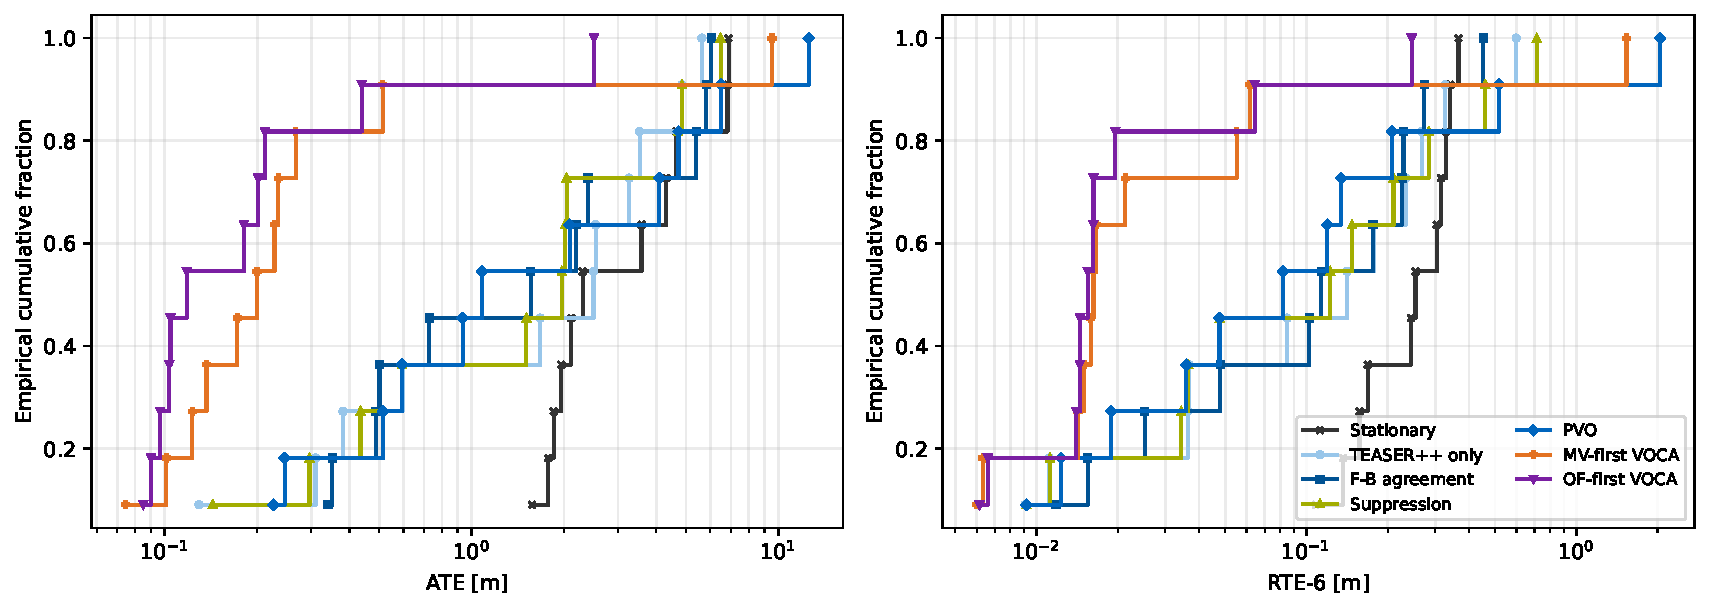
\includegraphics[width=\textwidth]{figures/evaluation/trajectory-error-ecdf}
  \caption[Distributions of full-sequence trajectory errors]{Empirical cumulative distributions over the eleven full-sequence ATE
  values (left) and RTE-6 values (right). The logarithmic horizontal axes retain
  the effect of both low-error sequences and large failures.}
  \label{fig:trajectory-error-ecdf}
\end{figure}

\subsection{Trajectory Geometry}\label{sec:trajectory-geometry}

The trajectory overlays illustrate the central feasibility result: motion
vectors alone can support reasonable camera-motion tracking.
The easy Machine Hall sequences give especially clear examples:
\autoref{fig:trajectory-emh01-separated} and
\autoref{fig:trajectory-emh02-separated} show close agreement with the
reference paths on EMH01 and EMH02. The medium EMH03 sequence and EV201
follow in \autoref{fig:trajectory-emh03-separated} and
\autoref{fig:trajectory-ev201-separated}. Their codec-only estimates recover
the broad shape of the reference route, with visible deviations in position
and vertical motion. Each method is shown separately against ground truth,
with common axes for comparison within a sequence.

These results demonstrate one way to recover useful trajectory geometry from
codec motion vectors and motivate further investigation of pixel-free VO.
Full-sequence PVO overlays for all eleven sequences, including failure cases,
are provided in \autoref{appendix:full-trajectories}; the temporal evidence for
failures is examined in \autoref{sec:failure-episodes}.

\begin{figure}[p]
  \centering
  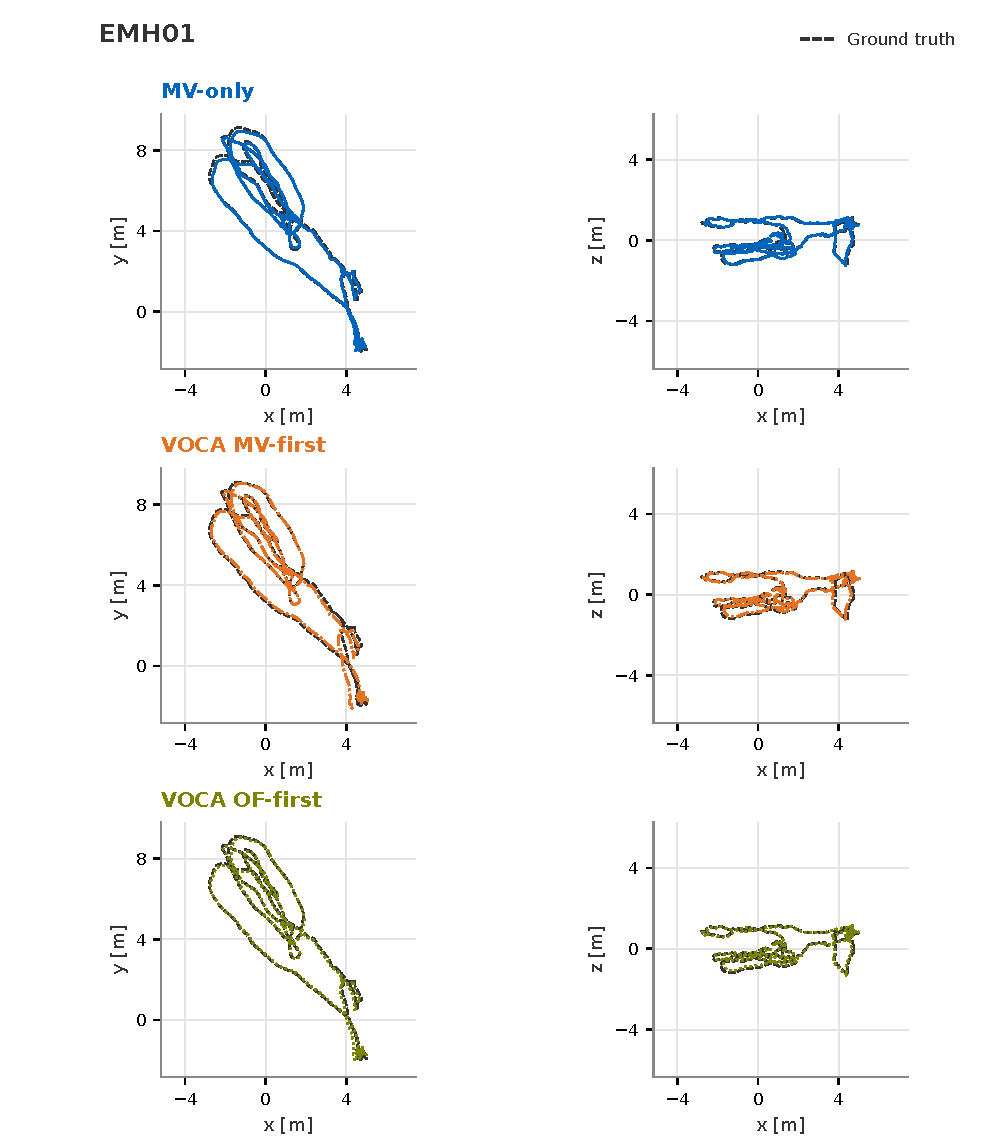
\includegraphics[width=\textwidth]{figures/evaluation/trajectory-emh01-separated.pdf}
  \caption[EMH01 trajectory comparison]{Full-sequence EMH01 trajectories. Top to bottom: MV-only,
  VOCA MV-first, and VOCA OF-first, each with ground truth. Left: $xy$;
  right: $xz$. All rows share the same spatial limits and metric scale.
  Each complete estimate uses its rigid alignment for ATE, shared between
  projections, without scale correction. All saved estimates are shown.}
  \label{fig:trajectory-emh01-separated}
\end{figure}

\begin{figure}[p]
  \centering
  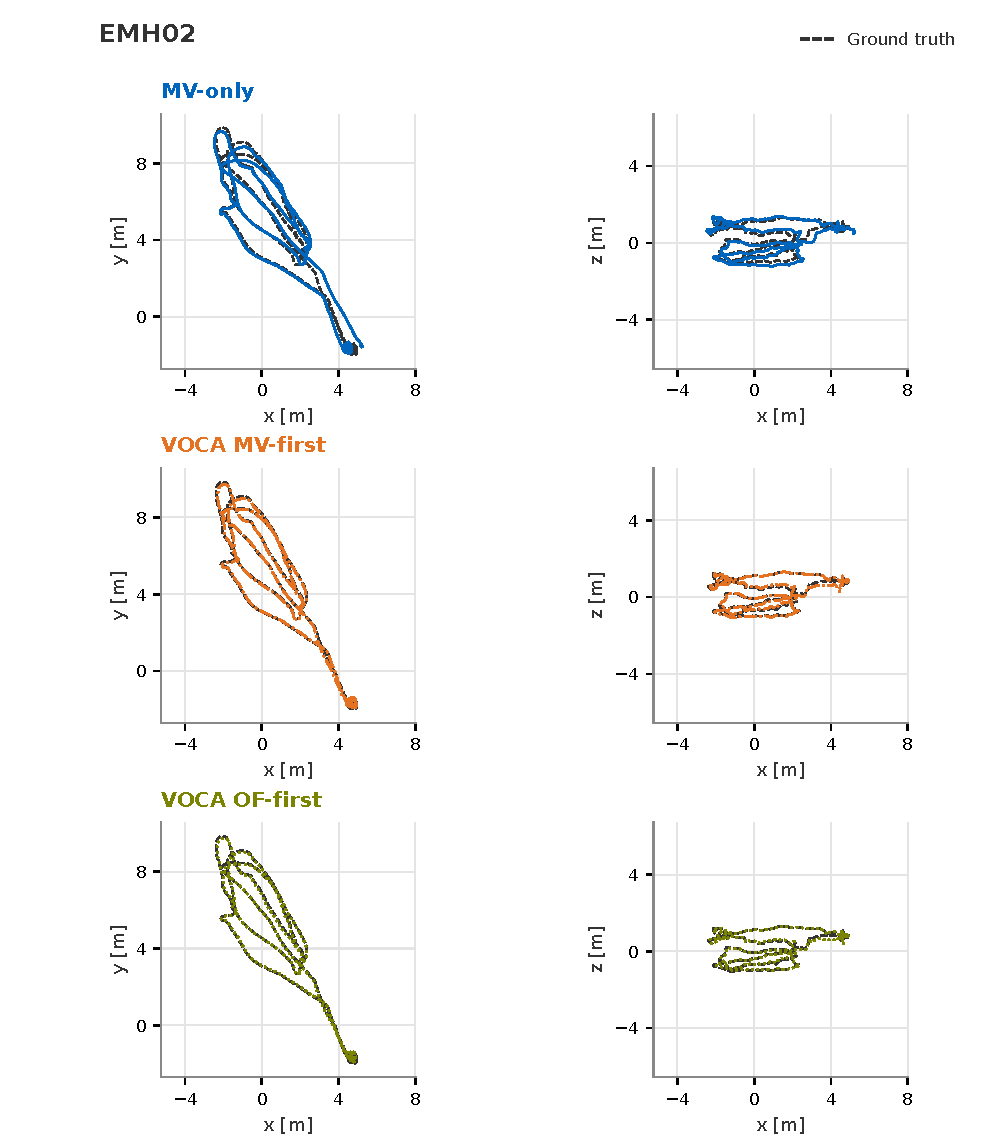
\includegraphics[width=\textwidth]{figures/evaluation/trajectory-emh02-separated.pdf}
  \caption[EMH02 trajectory comparison]{Full-sequence EMH02 trajectories. Top to bottom: MV-only,
  VOCA MV-first, and VOCA OF-first, each with ground truth. Left: $xy$;
  right: $xz$. Alignment and plotting conventions follow
  \autoref{fig:trajectory-emh01-separated}.}
  \label{fig:trajectory-emh02-separated}
\end{figure}

\begin{figure}[p]
  \centering
  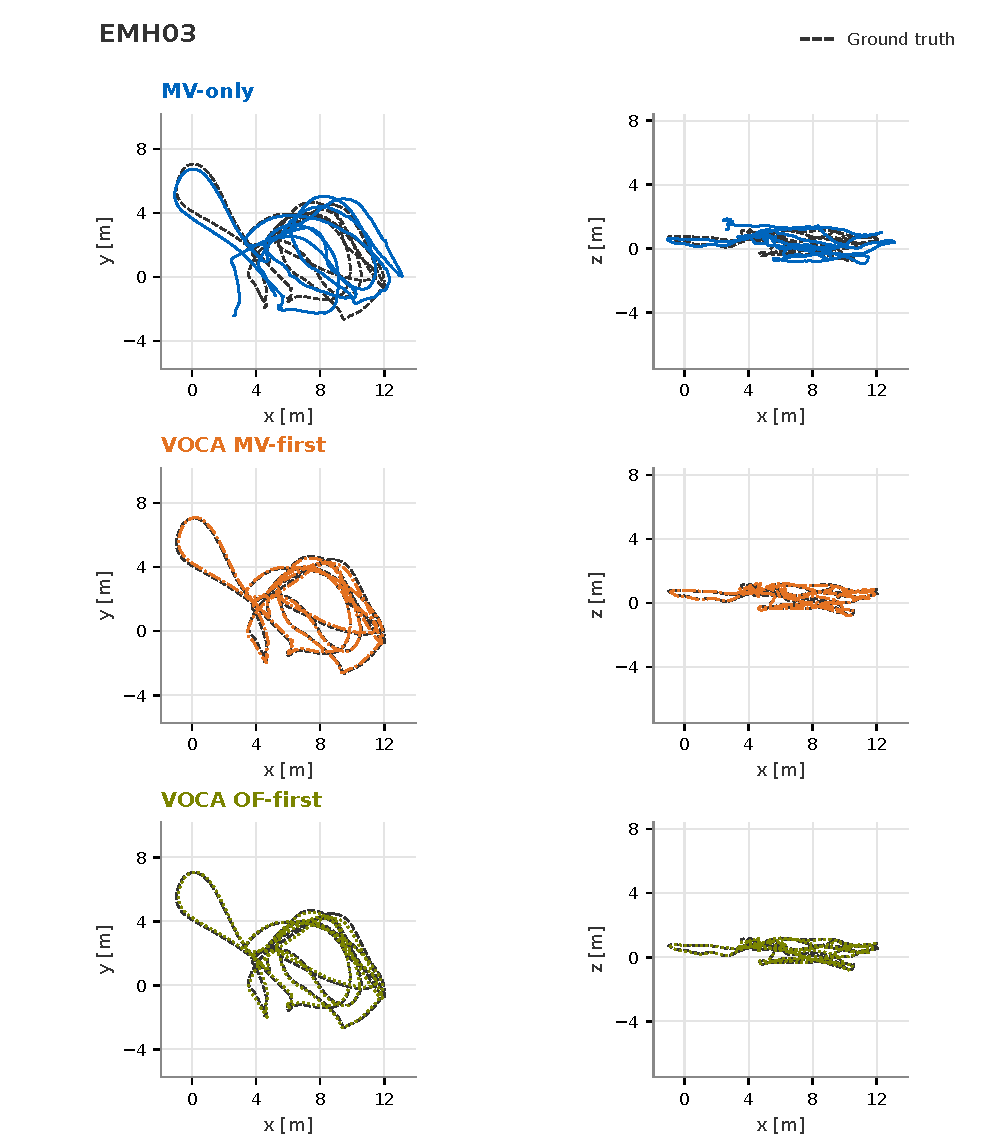
\includegraphics[width=\textwidth]{figures/evaluation/trajectory-emh03-separated.pdf}
  \caption[EMH03 trajectory comparison]{Full-sequence EMH03 trajectories. Top to bottom: MV-only,
  VOCA MV-first, and VOCA OF-first, each with ground truth. Left: $xy$;
  right: $xz$. Alignment and plotting conventions follow
  \autoref{fig:trajectory-emh01-separated}.}
  \label{fig:trajectory-emh03-separated}
\end{figure}

\begin{figure}[p]
  \centering
  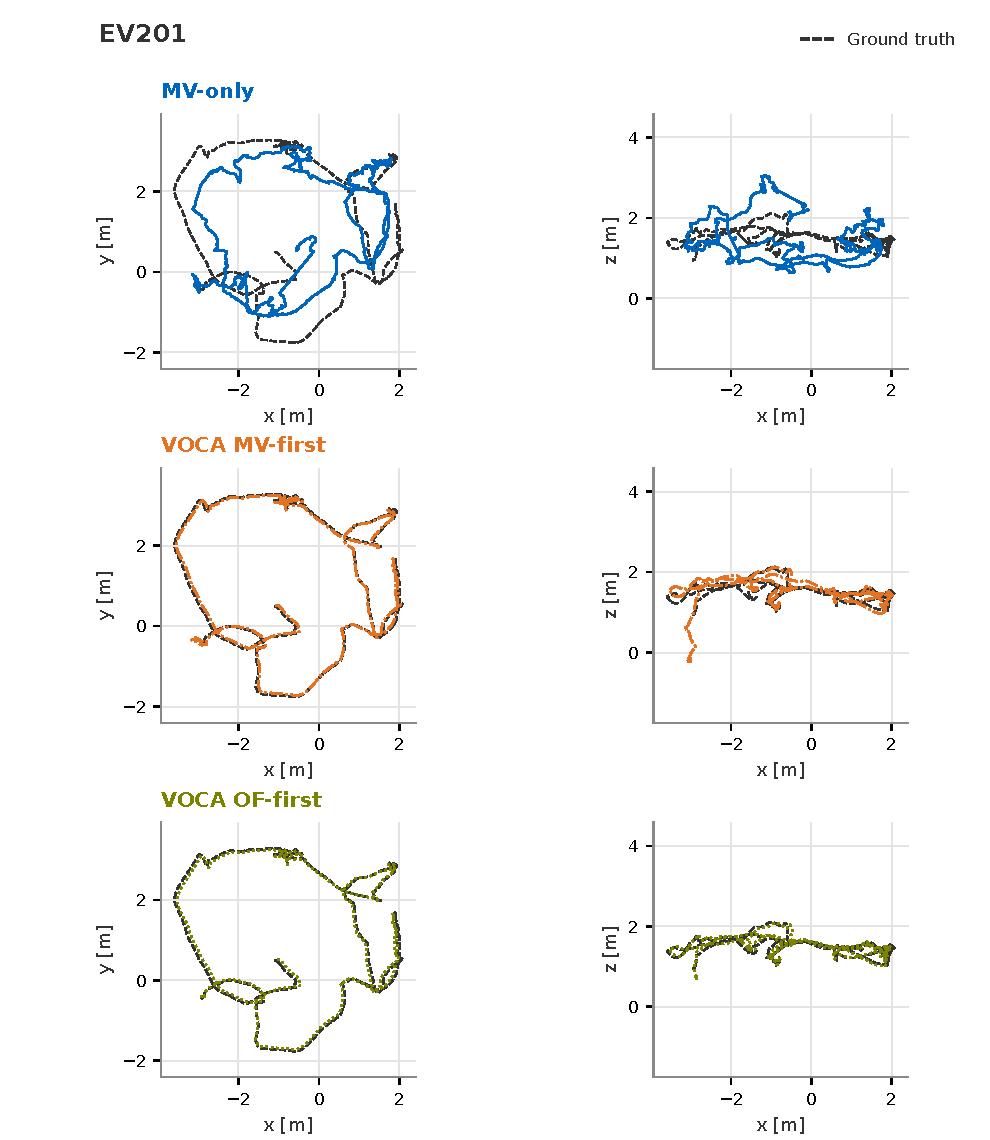
\includegraphics[width=\textwidth]{figures/evaluation/trajectory-ev201-separated.pdf}
  \caption[EV201 trajectory comparison]{Full-sequence EV201 trajectories. Top to bottom: MV-only,
  VOCA MV-first, and VOCA OF-first, each with ground truth. Left: $xy$;
  right: $xz$. Alignment and plotting conventions follow
  \autoref{fig:trajectory-emh01-separated}.}
  \label{fig:trajectory-ev201-separated}
\end{figure}

\clearpage

\section{Results by Sequence Difficulty}

For PVO, the easy sequences have a mean ATE of
\SI{0.500}{\metre} and a median of \SI{0.420}{\metre}. The corresponding values
are \SI{1.228}{\metre} and \SI{1.082}{\metre} for the medium sequences, and
\SI{6.968}{\metre} and \SI{5.609}{\metre} for the difficult sequences. Mean
RTE-6 rises from \SI{0.0306}{\metre} on easy sequences to
\SI{0.0971}{\metre} on medium and \SI{0.7035}{\metre} on difficult sequences.

These labels are descriptive groups, not uniformly spaced levels of numeric
difficulty. EV201, for example, is labelled easy but its codec-only ATE is higher
than that of the other three easy sequences. Conversely, local RTE-6 remains
relatively small on some trajectories whose global ATE is poor.

\begin{table}[htbp]
  \centering
  \caption[Trajectory and track statistics by sequence difficulty]{Trajectory and track statistics of PVO grouped by
  the EuRoC difficulty labels. Observations/frame counts confirmed
  anchor-camera observations pooled over input frames, not new identities or
  connected backend landmarks. Lifetimes are pooled over tracks;
  trajectory means and medians weight sequences equally.}
  \label{tab:difficulty-track-summary}
  \resizebox{\textwidth}{!}{%
  \begin{tabular}{@{}lrrrrrrrr@{}}
    \toprule
    & \multicolumn{2}{c}{ATE [m]} & \multicolumn{2}{c}{RTE-6 [m]}
    & & \multicolumn{3}{c}{Track lifetime} \\
    \cmidrule(lr){2-3}\cmidrule(lr){4-5}\cmidrule(l){7-9}
    Difficulty & Mean & Median & Mean & Median & Obs./frame
      & Mean [frames] & $\geq5$ [\%] & Maximum \\
    \midrule
    Easy      & 0.500 & 0.420 & 0.0306 & 0.0156 & 998.21 & 3.521 & 11.04 & 204 \\
    Medium    & 1.228 & 1.082 & 0.0971 & 0.0476 & 475.11 & 3.403 & 8.11 & 77 \\
    Difficult & 6.968 & 5.609 & 0.7035 & 0.3256 & 370.99 & 3.415 & 7.67 & 82 \\
    \bottomrule
  \end{tabular}}
\end{table}

\begin{figure}[htbp]
  \centering
  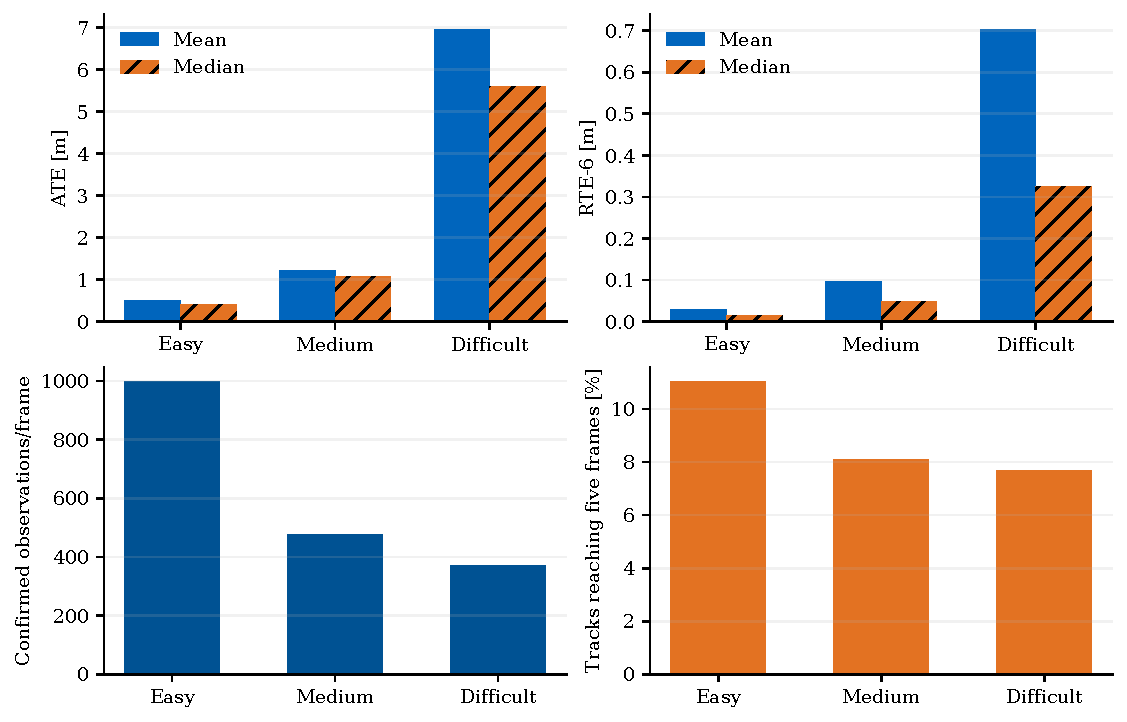
\includegraphics[width=\textwidth]{figures/evaluation/difficulty-summary}
  \caption[Trajectory errors and track support by sequence difficulty]{PVO trajectory errors and track support separated by
  EuRoC difficulty. Confirmed observation density decreases across the groups,
  while all three remain dominated by short tracks. The lifetime panel reports
  the proportion reaching at least five frames.}
  \label{fig:difficulty-summary}
\end{figure}

\clearpage

\section{Component Ablation}

\autoref{tab:component-ablation-ate} and
\autoref{tab:component-ablation-rte} give the full-sequence component results at
the original operating point and the selected PVO result. Bold marks the lowest
codec-only value in each row. ``Joint frontend'' uses the complete method at the
original settings; PVO uses the same components with selected reciprocal gates,
suppression distance, observation standard deviation, and Huber threshold.
PVO is included for comparison but is not another cell of the controlled
component ablation.

\begin{table}[htbp]
  \centering
  \caption[Component ablation: absolute trajectory error]{Full-sequence ATE for the codec-only component ablation, in metres.}
  \label{tab:component-ablation-ate}
  \resizebox{\textwidth}{!}{%
  \begin{tabular}{@{}lrrrrr@{}}
    \toprule
    Sequence & TEASER++ only & F-B agreement & Suppression & Joint frontend & PVO \\
    \midrule
    EMH01 & \textbf{0.129} & 0.488 & 0.143 & 0.232 & 0.246 \\
    EMH02 & 0.310 & 0.352 & 0.296 & \textbf{0.203} & 0.594 \\
    EMH03 & 3.261 & 1.559 & 1.508 & 1.569 & \textbf{1.082} \\
    EMH04 & \textbf{3.527} & 6.045 & 4.856 & 5.672 & 4.722 \\
    EMH05 & 5.629 & 5.401 & 4.706 & 5.318 & \textbf{4.089} \\
    EV101 & 0.381 & 0.340 & 0.434 & \textbf{0.223} & 0.226 \\
    EV102 & 0.596 & \textbf{0.501} & 0.594 & 0.622 & 0.514 \\
    EV103 & 2.536 & 2.196 & \textbf{2.019} & 3.406 & 12.565 \\
    EV201 & 1.673 & \textbf{0.727} & 1.968 & 0.899 & 0.935 \\
    EV202 & 2.495 & 2.392 & \textbf{2.040} & 2.671 & 2.087 \\
    EV203 & \textbf{4.842} & 5.817 & 6.479 & 7.635 & 6.497 \\
    \midrule
    Macro mean & 2.307 & 2.347 & \textbf{2.277} & 2.586 & 3.051 \\
    Median & 2.495 & 1.559 & 1.968 & 1.569 & \textbf{1.082} \\
    \bottomrule
  \end{tabular}}
\end{table}

\begin{table}[htbp]
  \centering
  \caption[Component ablation: six-frame relative translation error]{Full-sequence RTE-6 for the codec-only component ablation, in
  metres.}
  \label{tab:component-ablation-rte}
  \resizebox{\textwidth}{!}{%
  \begin{tabular}{@{}lrrrrr@{}}
    \toprule
    Sequence & TEASER++ only & F-B agreement & Suppression & Joint frontend & PVO \\
    \midrule
    EMH01 & \textbf{0.0091} & 0.0118 & 0.0092 & 0.0115 & 0.0092 \\
    EMH02 & \textbf{0.0112} & 0.0155 & 0.0112 & 0.0159 & 0.0123 \\
    EMH03 & 0.0848 & 0.1025 & 0.0477 & 0.0978 & \textbf{0.0476} \\
    EMH04 & 0.1779 & 0.1767 & 0.1476 & 0.1488 & \textbf{0.1344} \\
    EMH05 & 0.1414 & 0.2290 & 0.1226 & 0.1365 & \textbf{0.1195} \\
    EV101 & 0.0363 & 0.0252 & 0.0343 & 0.0190 & \textbf{0.0189} \\
    EV102 & 0.0368 & 0.0480 & 0.0365 & 0.0494 & \textbf{0.0359} \\
    EV103 & 0.3264 & \textbf{0.2262} & 0.2839 & 0.2585 & 2.0434 \\
    EV201 & 0.2674 & 0.1134 & 0.4599 & 0.1005 & \textbf{0.0818} \\
    EV202 & 0.2328 & 0.2735 & 0.2102 & 0.2564 & \textbf{0.2078} \\
    EV203 & 0.5989 & 0.4523 & 0.7135 & \textbf{0.4365} & 0.5169 \\
    \midrule
    Macro mean & 0.1748 & 0.1522 & 0.1888 & \textbf{0.1392} & 0.2934 \\
    Median & 0.1414 & 0.1134 & 0.1226 & 0.1005 & \textbf{0.0818} \\
    \bottomrule
  \end{tabular}}
\end{table}

\clearpage

PVO has the lowest median ATE and RTE-6 and the lowest RTE-6 on seven sequences.
Suppression at the original operating point retains the lowest macro mean ATE,
while the joint frontend at that point retains the lowest macro mean RTE-6. The
PVO macro means are dominated by the EV103 failure. Relative to TEASER++ only,
PVO lowers ATE on six sequences and RTE-6 on eight. The sequence rows make the
non-monotonic effect explicit: the selected parameters improve typical local
drift but do not eliminate large failures.

\section{Observation-Model Ablation}

The paired comparison in \autoref{tab:residual-ablation} uses the complete
selected PVO frontend and changes only the backend observation factor. The
rigid-flow residual has lower ATE on eight of eleven sequences and lower RTE-6
on seven. It also lowers both medians. The macro means favour absolute
reprojection because the rigid-flow run fails strongly on EV103, and absolute
reprojection is also better on EV203. The displacement formulation therefore
improves the typical sequence in this experiment but does not remove the
method's sequence-level failure modes.

\begin{table}[p]
  \centering
  \caption[Ablation of the observation model]{Full-sequence ablation of the observation model at the selected PVO
  operating point. All encoded inputs, frontend decisions, robust associations,
  loss parameters, and window settings are shared. Lower is better; bold marks
  the lower value within each metric.}
  \label{tab:residual-ablation}
  \begin{tabular}{@{}lrrrr@{}}
    \toprule
    & \multicolumn{2}{c}{ATE [m]} & \multicolumn{2}{c}{RTE-6 [m]} \\
    \cmidrule(lr){2-3}\cmidrule(l){4-5}
    Sequence & Absolute & Rigid flow & Absolute & Rigid flow \\
    \midrule
    EMH01 & 0.253 & \textbf{0.246} & \textbf{0.0089} & 0.0092 \\
    EMH02 & \textbf{0.482} & 0.594 & 0.0207 & \textbf{0.0123} \\
    EMH03 & 1.215 & \textbf{1.082} & 0.0488 & \textbf{0.0476} \\
    EMH04 & 4.960 & \textbf{4.722} & \textbf{0.1294} & 0.1344 \\
    EMH05 & 4.266 & \textbf{4.089} & 0.1279 & \textbf{0.1195} \\
    EV101 & 0.263 & \textbf{0.226} & 0.0219 & \textbf{0.0189} \\
    EV102 & 0.531 & \textbf{0.514} & 0.0393 & \textbf{0.0359} \\
    EV103 & \textbf{2.538} & 12.565 & \textbf{0.2910} & 2.0434 \\
    EV201 & 1.152 & \textbf{0.935} & 0.0824 & \textbf{0.0818} \\
    EV202 & 2.281 & \textbf{2.087} & 0.2621 & \textbf{0.2078} \\
    EV203 & \textbf{4.565} & 6.497 & \textbf{0.4264} & 0.5169 \\
    \midrule
    Macro mean & \textbf{2.046} & 3.051 & \textbf{0.1326} & 0.2934 \\
    Median & 1.215 & \textbf{1.082} & 0.0824 & \textbf{0.0818} \\
    \bottomrule
  \end{tabular}
\end{table}

\section{Track Length and Geometric Support}

Across all eleven sequences, PVO produces 5,230,916 confirmed
tracks. Their mean length is 3.48 frames, the median is 3, the 90th percentile is
4, the 95th percentile is 5, and the longest track spans 204 frames. Only
29.85\% survive for at least four frames, 9.92\% for at least five, 0.25\% for at
least ten, and 0.05\% for at least twenty. The method therefore creates
persistent identities, but the typical constraint has little multiview support.

No quantitative track-length comparison with the VOCA MV-first and OF-first
references is reported. The necessary lifetime instrumentation was evaluated in
a separate diagnostic build that did not reproduce the frozen reference
trajectories: its ATE on the first easy Machine Hall sequence differed from both
reference values. Retaining those track statistics would therefore mix
different operating points. The trajectory comparison in
\autoref{tab:euroc-ate} and \autoref{tab:euroc-rte6} remains valid because it
uses the archived frozen reference results directly.

The stereo-query yield also varies substantially by sequence. In PVO it is
13.48\% on EMH01, 13.56\% on EMH02, and 19.88\% on EV101, but falls to 1.99\%,
1.14\%, and 0.71\% on EV201 to EV203. Among observations with depth at
consecutive endpoints, the mean absolute depth change ranges from
\SI{0.0262}{\metre} to \SI{0.0424}{\metre}. This conditional statistic does not
measure the larger population for which one or both depths are absent.

\autoref{fig:stereo-depth-support} retains the individual sequence measurements
alongside the signed RTE-6 difference, PVO minus VOCA MV-first. The plot describes
which support measurements accompany each complete trajectory; it does not
locate a failure or identify its cause. In particular, similar full-sequence
track lifetimes can conceal a brief interruption or an extended period of
incorrect motion. \autoref{sec:failure-episodes} examines those events in their
temporal and visual context.

\begin{figure}[htbp]
  \centering
  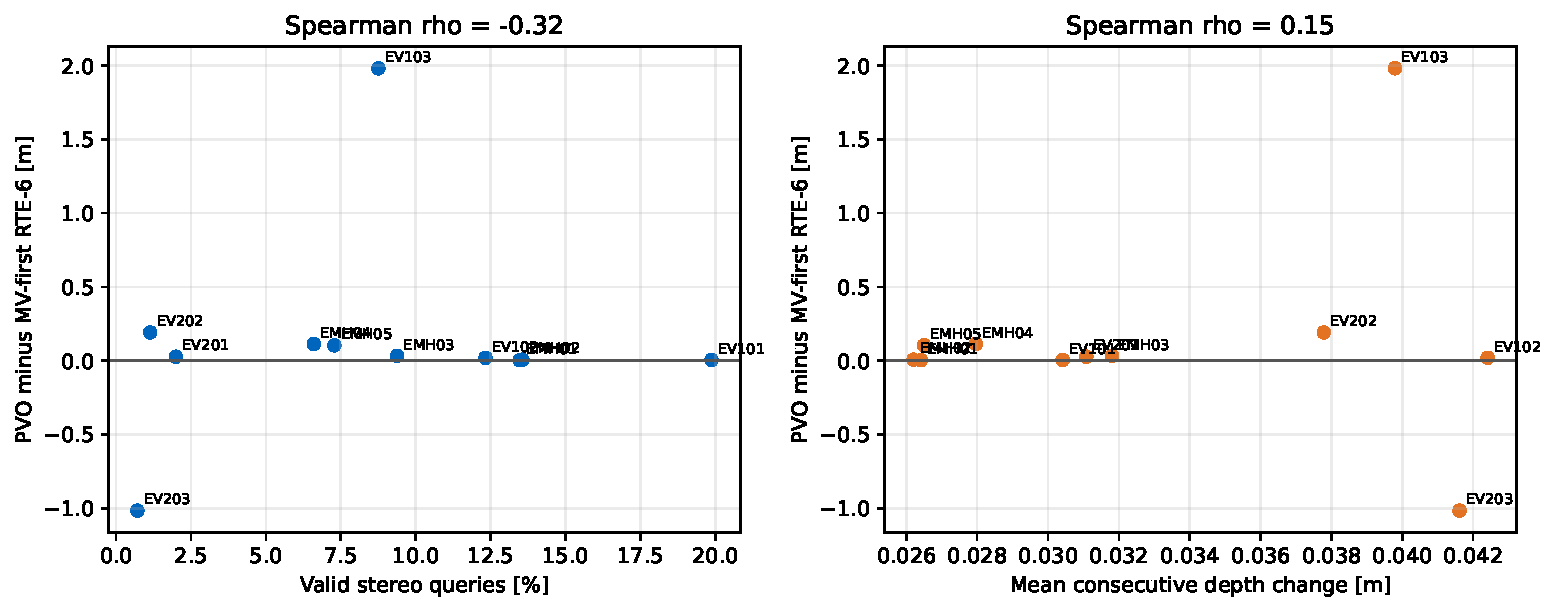
\includegraphics[width=\textwidth]{figures/evaluation/stereo-and-depth-support}
  \caption[Stereo support and relative translation error]{Valid-stereo rate (left) and mean absolute consecutive depth change
  (right) against the signed RTE-6 difference, PVO minus VOCA MV-first.
  Positive vertical values indicate greater PVO error. Labels identify the
  eleven sequence aggregates.}
  \label{fig:stereo-depth-support}
\end{figure}

\section{Coincidence with Conventional Image Structure}

The error-surface analysis in \autoref{eq:mv-error-hessian} provides the reason
for measuring this coincidence. Corner-like structure gives a block matching
cost curvature in two displacement directions, whereas an edge or weakly
textured support leaves at least one direction ambiguous. The following test
therefore measures whether filtering concentrates motion-vector support near
image structure that can condition translational matching; it does not label a
motion vector as geometrically correct.

Decoded images are used only in this offline diagnostic. The estimator itself
does not receive the Shi-Tomasi responses reported in
\autoref{tab:structure-support-all}. A motion-vector observation is counted as
structurally coincident when its exact prediction-block rectangle contains at
least one Shi-Tomasi corner. The rows give an ordered processing summary: raw anchor-camera
temporal vectors, vectors with valid stereo depth at both temporal endpoints,
reciprocal forward-backward candidates, TEASER++ survivors, and candidates
retained after age-prioritized suppression. The retained row also includes new
best-direction births awaiting reciprocal confirmation, so it branches from the
strict reciprocal path rather than forming its final subset.

\begin{table}[htbp]
  \centering
  \caption[Coincidence of codec supports and image corners]{Pooled full-sequence Shi-Tomasi coincidence across all eleven EuRoC
  sequences. Region support is the fraction of codec regions containing a
  corner; feature coverage is the fraction of detected corners lying in the
  union of those regions.}
  \label{tab:structure-support-all}
  \begin{tabular}{@{}lrrr@{}}
    \toprule
    Stage & Regions & Regions with corner & Corner coverage \\
    \midrule
    Raw temporal MVs & 84,675,992 & 30.59\% & 98.58\% \\
    Valid stereo depth & 41,353,155 & 37.45\% & 59.88\% \\
    Forward-backward candidates & 13,899,680 & 34.38\% & 32.48\% \\
    TEASER++ survivors & 6,856,688 & 39.57\% & 18.70\% \\
    Suppression-retained candidates & 23,057,616 & 44.54\% & 43.03\% \\
    \bottomrule
  \end{tabular}
\end{table}

Requiring stereo depth raises the region-level corner ratio from 30.59\% to
37.45\%. Contrary to a monotonic-enrichment hypothesis, reciprocal agreement
then lowers it to 34.38\%. TEASER++ raises it to 39.57\%, while the branched
suppression-retained pool reaches 44.54\%. The first four candidate counts fall
at every stage, so TEASER++ is both selective and more concentrated near
Shi-Tomasi structure than its reciprocal input. The feature-coverage column is
reported separately because the dense raw block union covers nearly every
corner even when individual regions are poorly localized.

\begin{figure}[htbp]
  \centering
  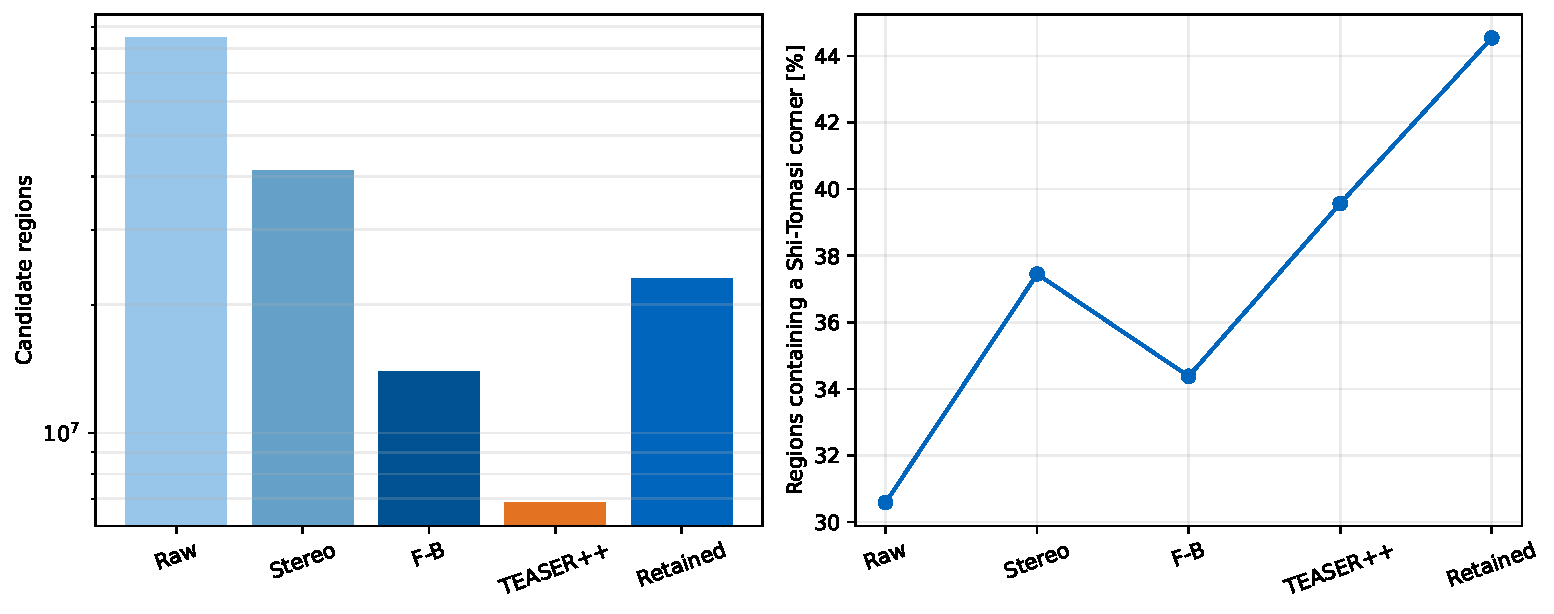
\includegraphics[width=\textwidth]{figures/evaluation/feature-support-funnel}
  \caption[Candidate count and structural support through filtering]{Candidate count and structural coincidence through the codec-only
  selection stages, pooled over all eleven sequences.}
  \label{fig:feature-support-funnel}
\end{figure}

Stricter Shi-Tomasi quality levels test whether the coincidence is limited to
weak corner responses. The same final codec supports are held fixed while only
the offline diagnostic threshold changes.

\begin{table}[htbp]
  \centering
  \caption[Corner coincidence at different detector thresholds]{Pooled coincidence of final codec supports with Shi-Tomasi corners
  at increasingly selective quality levels.}
  \label{tab:detector-threshold-support}
  \begin{tabular}{@{}lrrr@{}}
    \toprule
    Quality level & Corners & Regions with corner & Corner coverage \\
    \midrule
    0.01 & 18,921,761 & 44.54\% & 43.03\% \\
    0.05 & 8,365,939 & 25.51\% & 48.39\% \\
    0.10 & 5,076,456 & 17.64\% & 51.75\% \\
    \bottomrule
  \end{tabular}
\end{table}

At the default quality level, 44.54\% of retained regions contain a corner and
their union covers 43.03\% of the detected corners. As the diagnostic retains
only stronger corners, region coincidence falls because fewer responses exist,
but coverage of those responses rises to 51.75\%. This does not imply that a
retained codec region is a uniquely localized feature or that the estimator
observes the corner response.

\begin{figure}[htbp]
  \centering
  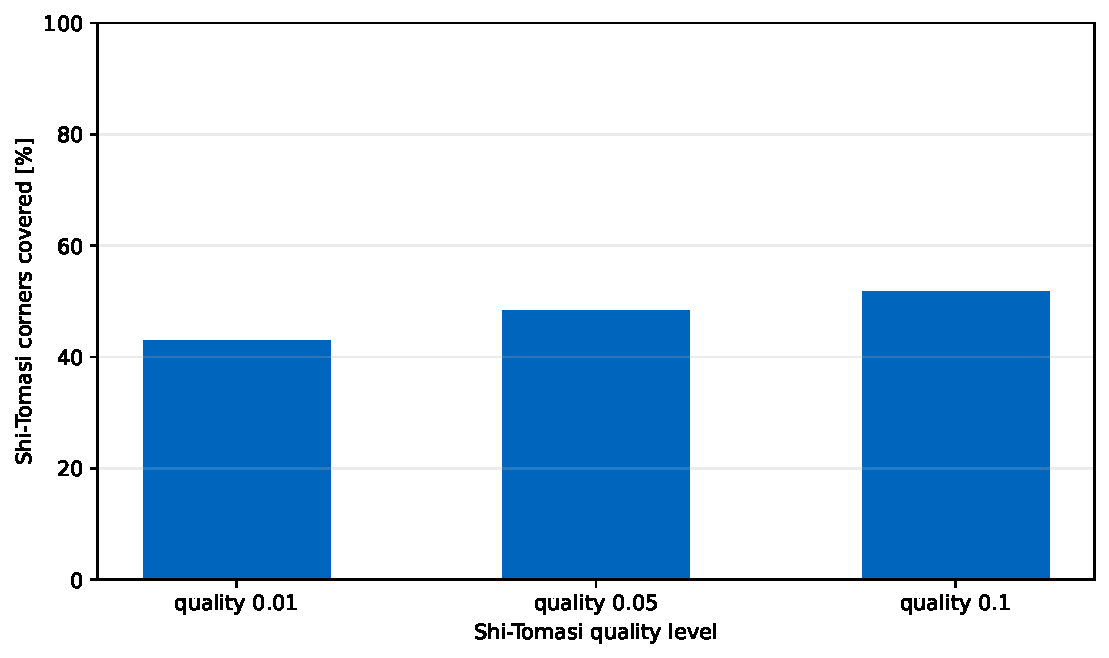
\includegraphics[width=0.8\textwidth]{figures/evaluation/shi-tomasi-threshold-support}
  \caption[Corner coverage at different detector thresholds]{Pooled Shi-Tomasi corner coverage by the fixed final codec supports
  at three detector quality levels.}
  \label{fig:shi-tomasi-threshold-support}
\end{figure}

\section{Reference Configurations}

The MV-first and OF-first VOCA configurations have access to image intensities
that are deliberately unavailable to the proposed estimator. They therefore
serve as higher-information operating points rather than objectives that the
PVO is expected to surpass. Their median ATE values are
\SI{0.200}{\metre} and \SI{0.118}{\metre}, respectively, compared with
\SI{1.082}{\metre} for PVO. Median RTE-6 is
\SI{0.0163}{\metre} for VOCA MV-first, \SI{0.0155}{\metre} for VOCA OF-first,
and \SI{0.0818}{\metre} for PVO.

The macro mean alone obscures reference failures: VOCA MV-first reaches
\SI{9.532}{\metre} ATE and \SI{1.534}{\metre} RTE-6 on EV203. The per-sequence
tables and empirical distributions are therefore retained rather than reducing
the benchmark to a single ranking. The central result is that codec side
information alone supports non-stationary estimates on a substantial part of the
benchmark, while a large and sequence-dependent accuracy gap remains.

% !TeX root = ../main.tex

\section{Failure Episodes}\label{sec:failure-episodes}

The full-sequence errors can arise through markedly different events. The
following cases follow the observations and estimated motion before, during,
and after an error. They use the selected PVO runs, with the paired absolute
residual and frozen VOCA OF-first results where indicated. The intervals were
selected by inspecting the complete saved trajectories; they are illustrative
episodes, not a partition of the benchmark or a model that predicts failure.
Times in the figures are relative to the first ground-truth-associated pose of
the sequence. Exact intervals and sources are retained with the analysis assets.

\subsection{Sustained Drift in a Dark, Sparsely Detailed View}

On EMH04, the view changes from machinery and pipework to a broad cabin roof
and the dark hall behind it. \autoref{fig:failure-emh04} follows this transition.
During a \SI{7.8}{\second} interval of sustained error, the images contain an
average of 124 Shi-Tomasi corners, compared with 751 in a later interval with
more visible machinery. RTE-6 falls from \SI{0.3584}{\metre} during the
degraded interval to \SI{0.0209}{\metre} in the later interval, even though mean
ground-truth path speed increases from \SI{1.19}{\metre\per\second} to
\SI{1.37}{\metre\per\second}. Faster translation therefore does not account
for the difference between these two views.

Codec candidates remain abundant. The degraded interval contains approximately
2229 temporal candidates per frame with valid stereo at both endpoints, and
217 current IDs per frame are connected to existing backend landmarks. These
counts do not collapse to zero. The estimated motion nevertheless becomes
incorrect in both magnitude and direction, and the first-pose-aligned
orientation error grows to approximately \SI{67}{\degree}. Once the view
improves, local translation error becomes small again, but much of the
orientation error remains. Local recovery therefore does not imply recovery
of the accumulated trajectory.

\begin{figure}[p]
  \centering
  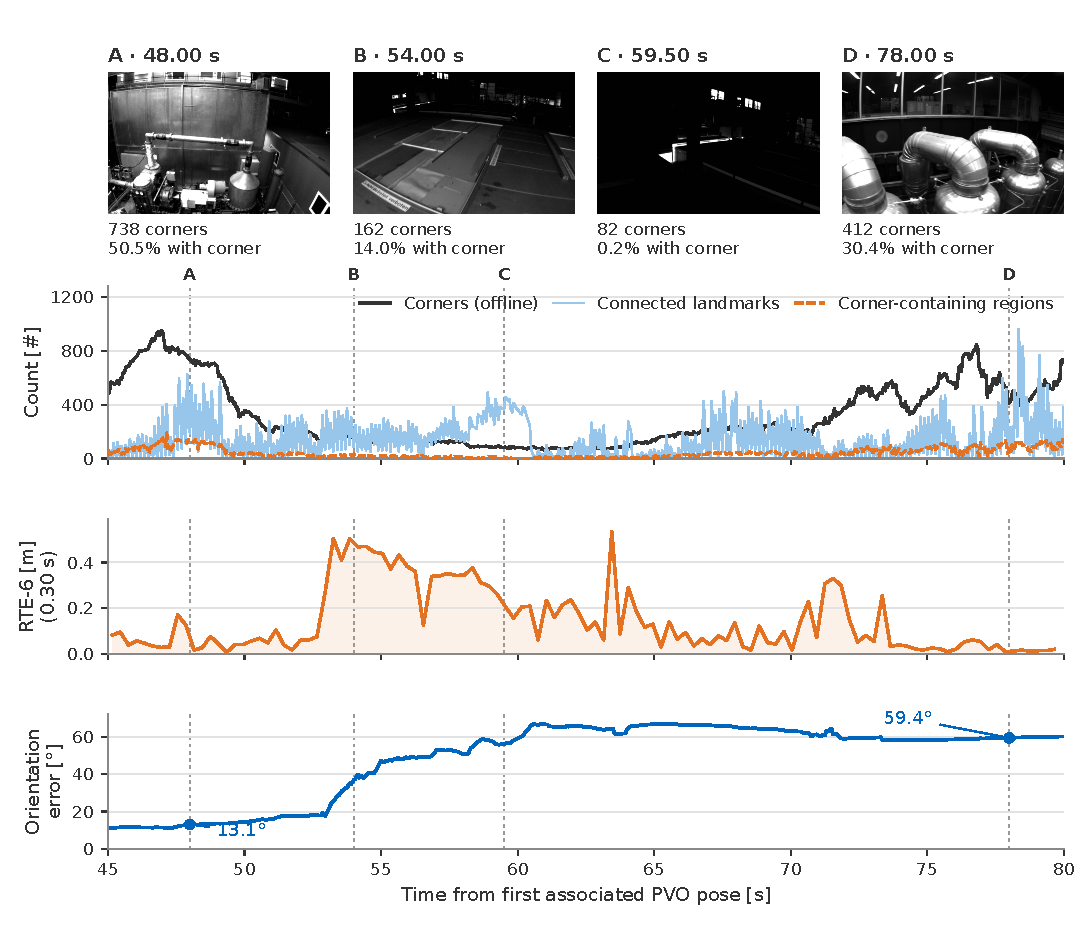
\includegraphics[width=\textwidth]{figures/evaluation/emh04-dark-scene-progression}
  \caption[Sustained drift on EMH04]{EMH04 before, during, and after sustained drift. Raw anchor-camera
  images are shown only for diagnosis. The synchronized traces distinguish
  changing image structure, local translation error, and persistent orientation
  error. Corner-containing regions are TEASER-stage MV destination blocks
  containing at least one offline Shi-Tomasi corner; the percentages divide
  their count by all logged TEASER-stage regions in each sampled frame.
  Connected IDs instead count observations linked to existing backend landmarks.
  Orientation error is aligned at the first pose, not over the full trajectory.}
  \label{fig:failure-emh04}
\end{figure}

The images and support measurements are consistent with less informative
codec predictions over broad surfaces and dark regions. The connection to
block-matching ambiguity follows the error-surface argument in
\autoref{eq:mv-error-hessian}~\cite{zhang2010subpixel,shi1994good}.
However, the recorded counts do not measure disparity accuracy or the spatial
rank of the retained point set. They cannot distinguish incorrect stereo
depth, temporal displacement bias, and unfavorable point geometry as the main
source of this episode. The fact that the paired absolute-residual run also
degrades in this interval provides an additional limit on its interpretation.

\subsection{A Brief Loss of Connections During Rapid Motion}

EMH03 contains a shorter event in which a six-frame interval reaches
\SI{0.4423}{\metre} RTE-6. It has an average of only 12.6 current IDs connected
to existing landmarks. A separate rapid-motion interval in the same sequence
has slightly greater translation and angular speed, yet its RTE-6 is only
\SI{0.0265}{\metre}. That interval retains 186.4 connected IDs on average.
The two image intervals contain similar numbers of detected corners, 656 and
670 per frame, respectively.

\begin{figure}[p]
  \centering
  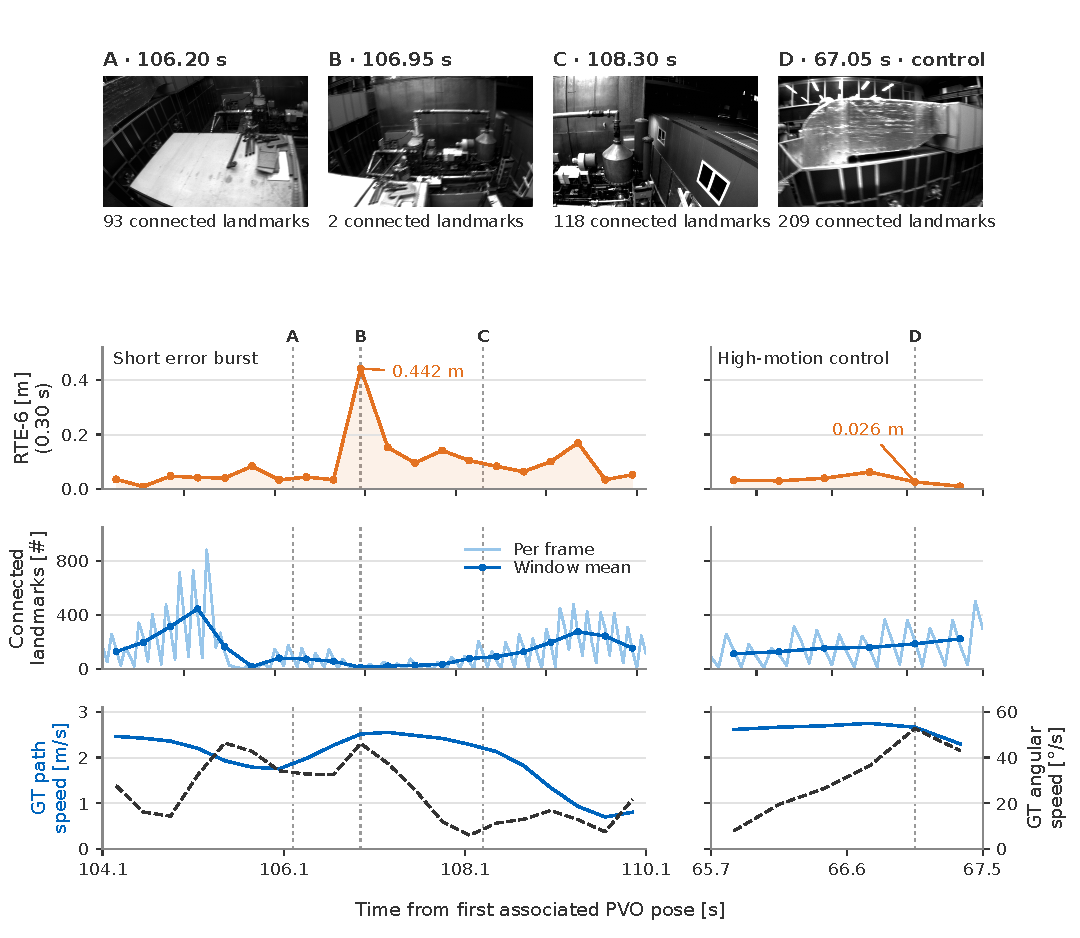
\includegraphics[width=\textwidth]{figures/evaluation/emh03-short-burst-and-motion-control}
  \caption[EMH03 error burst and rapid-motion comparison]{A short EMH03 error burst and a rapid-motion comparison interval.
  Connected IDs are current observations linked to existing backend landmarks.
  Similar image corner counts do not imply similar surviving temporal support;
  the faster comparison interval retains substantially more connections.}
  \label{fig:failure-emh03}
\end{figure}

This comparison separates the availability of visible structure from its
conversion into persistent observations. The failed interval is not simply
the faster or less corner-rich of the two. Its small connected set coincides
with a large local error, although the archived counters do not identify which
individual candidate losses produced that set. The absolute-residual run has
almost the same error in the burst, \SI{0.4397}{\metre}, which again indicates
that replacing rigid flow alone does not remove the event.

\subsection{Missing Temporal Observations, a Pose Jump, and a Stall}

EV103 illustrates a discontinuity rather than gradual drift. The view
approaches a bright window beside a broad dark partition. Visible corners and
emitted track IDs decrease. Inspection of the encoded streams also identifies
an I-frame in each direction at the endpoints of one temporal transition,
leaving no ordinary temporal MVs for that connection. Three frames later,
the estimated pose jumps by \SI{37.716}{\metre} and rotates by
\SI{174.42}{\degree} in one frame. Ground truth changes by only
\SI{0.050}{\metre} and \SI{0.77}{\degree}. At the jump, only two current IDs
are connected to existing landmarks; the optimizer records eight iterations,
six of them rejected.

\begin{figure}[p]
  \centering
  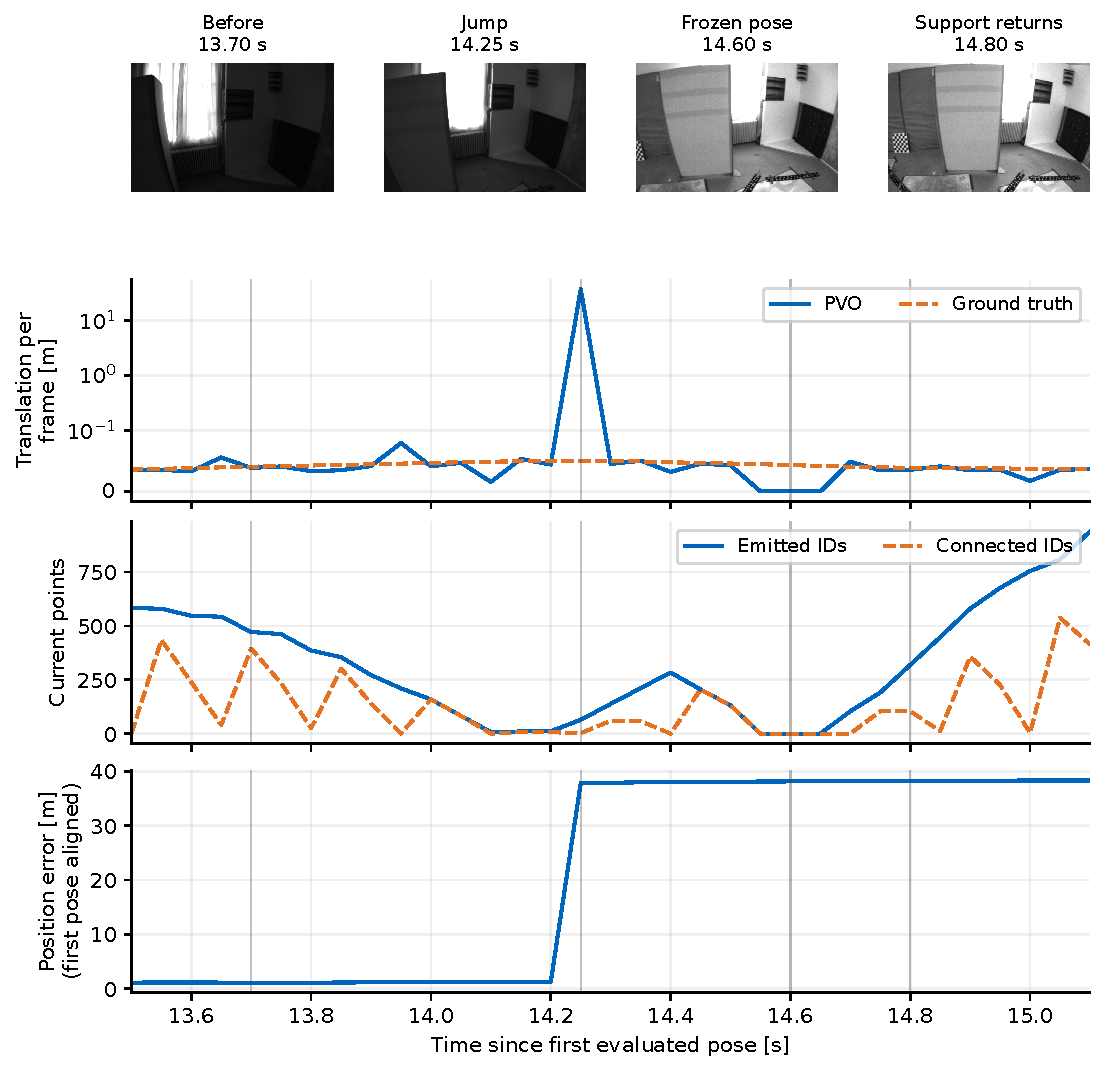
\includegraphics[width=\textwidth]{figures/evaluation/failure-ev103-jump}
  \caption[Catastrophic pose update on EV103]{EV103 around a catastrophic pose update. Per-frame translation uses
  a symmetric logarithmic axis so that ordinary motion, the large jump, and
  zero-motion outputs remain visible. The lower panels show the temporary loss
  of frontend support and the persistent position error after support returns.
  The sampled images are offline diagnostics.}
  \label{fig:failure-ev103}
\end{figure}

A subsequent transition again lacks temporal MVs in both directions. The
frontend then emits zero points for three consecutive frames and the pose
remains exactly unchanged, although ground truth moves approximately
\SI{0.04}{\metre} per frame. Image corners have already returned to at least
350 per frame. Raw MV candidates return after the missing transition, but no
candidate survives the logged stage requiring filtering and valid stereo at
both endpoints for the next two frames. These records locate the loss within
the processing chain; they do not isolate the median filter from stereo lookup
as its cause. Connections subsequently return, while the accumulated position
error remains approximately \SI{38}{\metre}.

The I-frames explain the observed absence of temporal vectors at particular
transitions, not the complete sequence of errors. The catastrophic update
itself occurs on a P-frame, and the shortage of usable observations extends
beyond the I-frame. The containing six-frame window contributes 98.6\% of
the full sequence's sum of squared six-frame translation errors. Its RTE-6 is
\SI{37.8510}{\metre}, compared with \SI{0.4066}{\metre} in the paired
absolute-residual run. This episode exposes a strong difference in how the
backends respond to the available observations; it does not show that every
large PVO error has the same origin.

\subsection{Low-Motion Errors and a Textured Counterexample}

EV202 contains consecutive estimated translations of \SI{1.117}{\metre} and
\SI{0.895}{\metre} while ground truth moves only \SI{0.013}{\metre} in each
frame. The images change little and show fabric-covered blocks, a plain wall,
and a small cart. Only three and two IDs, respectively, connect to existing
landmarks. At the first jump, 2919 raw MV regions and 541 stereo-valid temporal
candidates are still available, but only 25 reciprocal candidates and four
candidates passing the fitted rigid-model gate remain. This is another case
in which many initial observations do not translate into substantial temporal
support.

A later EV202 event provides a counterexample to using image corner count as a
sufficient indicator. A close, textured fabric surface dominates the view and
1640 corners are detected, yet the estimated translation is
\SI{0.752}{\metre} against a ground-truth step of \SI{0.015}{\metre}. Only six
IDs connect to existing landmarks. Conversely, a separate six-frame interval
with an average of 7.4 connected IDs has RTE-6 of only \SI{0.0376}{\metre}.
Neither high corner count nor low connection count alone determines the
outcome. Supplementary images and per-frame values are given in
\autoref{appendix:failure-episode-details}.

\subsection{What the Paired Residual Comparison Establishes}

\autoref{tab:episode-residual-comparison} compares identical timestamp
intervals from PVO, its absolute-residual ablation, and the frozen VOCA
OF-first reference. The two PVO runs share encoded inputs and frontend settings,
including the robust association procedure. EMH03's brief burst and EMH04's sustained error
remain under absolute reprojection. EV103's catastrophic amplification is much
smaller with absolute reprojection, as is EV202's textured-view error.
However, the EV202 jump at \SI{38.30}{\second} becomes larger. The observation
model thus changes the response to particular
correspondence sets without providing a universal safeguard. The low OF-first
errors on the same intervals show that the camera sequences still contain
information from which the richer reference can recover motion.

\begin{table}[htbp]
  \centering
  \caption[Observation-model comparison over failure episodes]{RTE-6 in metres; lower is better. Entries report
  RMSE over the listed non-overlapping windows. Absolute changes PVO's
  observation model; OF-first is the frozen pixel-refined reference. The
  EV202 middle jump is at \SI{38.30}{\second}, distinct from the later
  textured-view event.}
  \label{tab:episode-residual-comparison}
  \begin{tabular}{@{}lrrrr@{}}
\toprule
Episode & Windows & PVO [m] & Absolute [m] & OF-first [m] \\
\midrule
EMH03 burst & 1 & 0.4423 & 0.4397 & 0.0151 \\
EMH04 dark view & 26 & 0.3584 & 0.3719 & 0.0150 \\
EMH04 recovery & 23 & 0.0209 & 0.0270 & 0.0156 \\
EV103 jump & 1 & 37.8510 & 0.4066 & 0.0322 \\
EV202 early jumps & 1 & 1.3830 & 1.0851 & 0.0037 \\
EV202 middle jump & 1 & 1.1206 & 2.9941 & 0.0353 \\
EV202 textured view & 1 & 0.8402 & 0.2241 & 0.0019 \\
\bottomrule
\end{tabular}

\end{table}


% !TeX root = ../main.tex

\chapter{Discussion}\label{chapter:discussion}

\section{Answers to the Research Questions}

\paragraph{RQ1: remaining trajectory accuracy.}
The accuracy difference from the closest higher-information reference is
reported directly. For an error measure $e$, let
\begin{equation}
  \Delta e_{\mathrm{abs}} = e_{\mathrm{PVO}}-e_{\mathrm{MV\text{-}first}},
  \qquad
  \Delta e_{\mathrm{rel}} =
  100\frac{e_{\mathrm{PVO}}-e_{\mathrm{MV\text{-}first}}}
  {e_{\mathrm{MV\text{-}first}}}.
  \label{eq:pvo-reference-error-difference}
\end{equation}
Positive values mean that PVO has greater error. For the easy group, the
differences between group macro means are \SI{0.334}{\metre} and 201.3\% for ATE, and
\SI{0.0101}{\metre} and 49.6\% for RTE-6. The small RTE-6 difference shows that
local motion can remain close to the MV-first reference on easier motion even
when the accumulated trajectory differs more strongly. Across the benchmark,
the gap grows and is dominated by several difficult sequences; EV203 is the
exception on which PVO has lower ATE and RTE-6 than MV-first. PVO nevertheless
improves on the stationary baseline in both metrics on nine of eleven
sequences. The relative differences must be read together with the absolute
ones because division by a small reference error can produce a large
percentage from a modest metric displacement.

\begin{table}[htbp]
  \centering
  \caption[Trajectory-error differences between PVO and VOCA MV-first]{Absolute and percentage differences between the group macro means
  of PVO and VOCA MV-first. Positive values indicate greater PVO error.
  Difficulty groups follow the EuRoC sequence labels.}
  \label{tab:pvo-mv-first-error-differences}
  \begin{tabular}{@{}lrrrr@{}}
    \toprule
    Group & $\Delta$ATE [m] & $\Delta$ATE [\%] & $\Delta$RTE-6 [m] & $\Delta$RTE-6 [\%] \\
    \midrule
    Easy & 0.334 & 201.3 & 0.0101 & 49.6 \\
    Medium & 1.091 & 796.6 & 0.0811 & 507.3 \\
    Difficult & 4.341 & 165.3 & 0.2954 & 72.4 \\
    All sequences & 1.998 & 189.7 & 0.1332 & 83.2 \\
    \bottomrule
  \end{tabular}
\end{table}

\paragraph{RQ2: stereo-temporal persistence and support.}
Persistent identities can be assembled without pixel descriptors, but their
typical lifetime is short. Across the benchmark, PVO confirms
5,230,916 tracks with a median length of three frames and a 95th percentile of
five frames. Only 9.92\% reach five frames. Stereo support is likewise uneven:
Between 13.48\% and 19.88\% of queries return a match on EMH01, EMH02, and EV101, whereas
the rate is at most 1.99\% on EV201 to EV203. In the separate structure
diagnostic, the proportion of codec supports that contain a Shi-Tomasi corner
changes across valid stereo, reciprocal agreement, robust registration, and
suppression: 30.59\% for raw vectors, 37.45\% with valid endpoint depth, 34.38\%
after reciprocal agreement, 39.57\% after TEASER++, and 44.54\% in the branched
suppression-retained pool. Robust registration therefore concentrates its input
near two-directional image structure, but most individual tracks still offer
little multiview support.

\paragraph{RQ3: properties associated with failure.}
The episode analysis identifies several distinct events
(\autoref{sec:failure-episodes}). EMH04 develops sustained drift while the
view becomes dark and sparsely detailed, despite abundant stereo-valid
candidates. EMH03 has a brief burst during rapid motion with substantially
fewer retained connections than another, slightly faster interval with similar
corner support. EV103 suffers a catastrophic pose update, temporary stationary
outputs, and recovery of local motion without recovery of the accumulated
trajectory. EV202 supplies both low-motion jumps and a failure in a
corner-rich view. Visible structure, observation availability, and usable
temporal geometry are therefore different quantities.

The paired residual comparison further limits the explanations. EMH03 and
EMH04 retain their selected failures with absolute reprojection, while EV103's
catastrophic error is much smaller. Another EV202 jump is worse with absolute
reprojection. The recorded events establish when support is lost and how the
estimated motion changes; they do not identify one cause shared by every
sequence. Track lifetime and consecutive-depth summaries provide context but
cannot explain an individual event without its temporal evidence.

\section{Operating Envelope}

The clearest feasibility evidence is the recovered trajectory geometry on the
easy sequences, particularly the Machine Hall views in
\autoref{sec:trajectory-geometry}. The reported PVO results on EMH01 and EV101
also show low accumulated error. Improvement over a stationary prediction on
all four easy sequences provides a broader check that the estimates contain
motion information. PVO also improves on all three medium sequences, although
the quality varies substantially. The EV202 margin is small: \SI{2.087}{\metre} ATE and
\SI{0.2078}{\metre} RTE-6 versus stationary values of \SI{2.111}{\metre} and
\SI{0.2441}{\metre}. The difficult set is mixed rather than uniformly
unsuccessful, with improvements on EMH04 and EMH05 but not on EV103 or EV203.

This grouping should not be read as a calibrated scale of codec difficulty.
The EuRoC labels summarize the original sequence challenge, not the quality of
H.264 prediction blocks or compressed-domain stereo. EV201 is labelled easy yet
has substantially lower stereo yield than the other easy sequences. Conversely,
local drift can remain moderate while small errors accumulate into a poor
global trajectory. The evidence supports an operating envelope for the fixed
EuRoC cameras, calibrations, and encoder configuration; it does not establish
the same boundary for other cameras, frame rates, codecs, or encoder searches.

\section{Track Persistence and Geometric Support}

The three-observation median is only one observation longer than the provisional
period required for confirmation. Consequently, most accepted landmarks supply
little temporal baseline before disappearing. This limits the number of views
that can jointly constrain a point and reduces the opportunity to average block
quantization and stereo-depth errors. The small tail of longer tracks shows that
identity persistence is possible, with a maximum of 204 frames, but that tail is
too sparse to characterize the typical backend input.

Stereo availability is one bottleneck rather than a complete explanation. A
continuation needs geometrically acceptable support, and a new identity also
needs depth at both endpoints before it can enter the robust 3D registration.
The low query yield on EV201 to EV203 therefore removes many potential
associations early. Conditional consecutive-depth changes are small among
points for which both depths exist, but this statistic says nothing about the
larger set with missing depth. Track loss can additionally reduce the connected
landmark ratio and request keyframes more frequently. Standard window
optimization and marginalization preserve information from accepted factors,
but they cannot recreate missing multiview observations.

The offline structure analysis provides a complementary result. Requiring valid
stereo at both endpoints, reciprocal agreement, and TEASER++ consensus changes
the fraction of regions containing a Shi-Tomasi corner at each stage. This
indicates whether geometric selection concentrates observations near
two-directional image structure without explicitly detecting it. It does not
show that each codec support contains one uniquely localized physical point,
and the diagnostic corner coordinates are never used by the estimator.

A quantitative lifetime comparison with the VOCA MV-first and OF-first
configurations is deliberately omitted. The diagnostic build instrumented for
track lifetimes did not reproduce their frozen trajectories, so its counters
would not describe the same configurations as the ATE and RTE-6 tables. The
qualitative expectation that pixel-refined tracking supplies
more precisely localized and longer-lived observations remains plausible, but
is not used here as a measured result.

\section{Error Modes}

The observed failures differ both in duration and in their relation to support.
EMH04 continues estimating motion with many observations but accumulates a large
orientation error. EV103's full-sequence RTE-6 is dominated by one catastrophic
window, followed by a period without emitted observations. These require
different explanations: the first calls into question the information supplied
by the surviving geometry, whereas the second also exposes the estimator's
response to an abrupt shortage of connections. Neither can be adequately
described by the full-sequence mean track length.

The observation-model ablation adds the same qualification at the backend.
Rigid flow lowers ATE on eight sequences, RTE-6 on seven, and both medians, but
its EV103 failure makes both macro means worse than absolute reprojection
(\autoref{tab:residual-ablation}). Replacing eligible absolute factors with
displacement factors lowers the median errors in this experiment, while
absolute initialization and fallback observations remain part of the estimator.
The replacement does not by itself guard against an erroneous correspondence
set or a poorly conditioned trajectory.

Two observation-level failures are directly visible before the later gates are
applied. First, local codec support can disappear while the tracked image
structure remains visible and raw temporal vectors remain elsewhere
(\autoref{fig:mv-abrupt-stop-example}). The responsible encoder decision is
unresolved in this example. Second, a codec block and its vector can
remain available while a localized appearance inside the source block is no
longer contained by the predicted destination block
(\autoref{fig:mv-feature-departure-example}). The latter is possible because the
encoder optimizes prediction of an extended block rather than persistence of a
particular scene point. These cases explain why raw-vector availability alone
does not establish a valid feature track.

In the separate EV103 episode, frame-type inspection identifies I-frames at the
relevant endpoints in both encoding directions, explaining the absence of ordinary
temporal vectors for that transition. Subsequent
P-frames restore raw candidates before useful frontend support returns. This
distinguishes an identified input interruption from the later losses whose
individual causes are not recorded. Similarly, EMH04's dark views suggest
ambiguous block predictions, but the saved logs cannot separate temporal-vector
bias from incorrect depth or an unfavorable distribution of points.

TEASER++ success does not by itself resolve those uncertainties. Its role is to
find a rigid transformation consistent with a subset of putative
associations~\cite{yang2020teaser}; such consistency does not independently
establish correspondence to the true scene. The implementation reports
successful registration throughout EMH04 even while the trajectory diverges.
Additional per-frame inlier geometry and residual diagnostics would be needed
to assess conditioning or identify coherent incorrect associations. The
present evidence does not establish that moving objects, calibration error,
or a particular depth distribution caused these episodes.

The median filter targets isolated compression artefacts, reciprocal agreement
tests temporal reversibility, TEASER++ rejects inconsistent 3D pairs, and
age-prioritized suppression removes indistinguishable duplicate support. These
stages address different symptoms. Their non-monotonic ablation results suggest
that stricter rejection can also discard useful constraints. The case studies
show where these distinctions matter, while identifying questions that the
available diagnostics cannot answer.

\section{Meaning of Pixel-Free Operation}

The information restriction applies to the tracking frontend and pose estimator. They
consume H.264 motion-vector side data, prediction-block geometry, timestamps,
camera calibration, rectification transforms, and validity masks. They do not
load decoded intensities, build image pyramids, detect corners, evaluate patches,
compute descriptors, or apply a photometric residual. Shi-Tomasi and blur
measurements are computed only after evaluation for diagnosis.

The restriction does not claim that the entire data-production process is
image-free. Decoded stereo images are remapped during offline rectification and
are then supplied to the video encoder. This conventional preprocessing creates
the H.264 streams on which the experiment operates. The resulting statement is
therefore precise: after calibrated offline rectification and encoding,
the frontend and pose estimator use codec side information and geometry without
consulting image intensities. The extraction software used here decodes frames
and reconstructs images internally, but does not forward those pixels to the
tracking frontend.

\section{Placement of Analysis and Transmission}\label{sec:cta-compatibility}

The communication boundary can be placed at several stages of the codec-based
frontend. Sending the required coded streams follows CTA: the capturing device
encodes, and the receiver extracts motion vectors and estimates camera motion.
Conventional CTA follows decoding with image-based feature extraction or
tracking~\cite{hofer2023h264cta}; here the frontend uses codec metadata directly.

Alternatively, the capturing device could extract the vectors and perform some
of the correspondence filtering before transmission. It could send temporal
and stereo observations for the remaining geometric checks, or run the frontend
locally and send confirmed observations to a remote backend. Analysis would then
precede the compression and transmission of the geometric data, giving an
ATC-like allocation of work while retaining codec-derived measurements. These
options extend the processing--communication choice described in the CTA--ATC
literature~\cite{redondi2016cta} to different stages of this frontend.

The transmitted representation must preserve the information needed after the
chosen boundary. Early motion-vector observations require block support,
reference information, timestamps, and calibrated geometry. A later split at
the frontend output would require shared calibration, consistent track identities,
per-camera coordinates, measured displacements, and predecessor timestamps,
with frontend and backend state maintained on their respective devices.
Filtering reduces the set of retained candidates, but the resulting bitrate also
depends on their metadata and encoding. The experiments do not implement or
measure these transport alternatives.

The evaluated input consists of two forward temporal streams, two reversed
temporal streams, and twelve shifted stereo streams. Preparing those additional
encodings has a cost. Two-pass temporal encoding and the current reversal of
complete frame lists make preparation an offline procedure, despite the
single-reference, B-frame-free prediction structure within each stream.
A live deployment must establish how the observations are generated and
delivered within its latency and throughput budget. Efficient metadata
extraction must also account for the pixel reconstruction performed by the
current decoder.

Passthrough+ motivates dedicated codec hardware with platform-specific power
budgets~\cite{chaurasia2020passthrough}. The present software-encoded experiments
establish geometric feasibility. Net energy savings depend on all preparation,
communication, extraction, and estimation. Reusing motion from an already
required stream has a different incremental cost from generating extra stereo
encodings. Sending an unchanged stream also preserves its bitrate; filtering
and transmitting geometric observations is a separate design choice.

\section{Validity and Limitations}

The evaluation covers all eleven EuRoC sequences, but only one benchmark, one
stereo camera family, and the provided calibrations. The result is also tied to
FFmpeg 4.4.2, \texttt{libx264}, H.264 High profile, the fixed temporal encoding,
and the twelve shifted I-P-P stereo streams. Hardware encoders or other search,
partition, bitrate, GOP, and colour-format choices may expose different motion
vectors. Passthrough+'s hardware mosaic, densification, pose-assisted temporal
depth propagation, and rendering stages are not reproduced. In particular, the
original full proxy assumes headset poses from an independent SLAM system,
which would violate the information restriction here. The stereo component is
therefore an adaptation rather than a complete replication of that system.

The selected PVO parameters were chosen after a bounded twelve-candidate sweep
on the same eleven sequences used for reporting. The final tables exclude
abandoned searches, but the evaluation is therefore not an independently
held-out benchmark study. The failure episodes are also selected retrospectively
and do not estimate the prevalence of a failure mechanism. Their successful
comparisons and counterexamples constrain the interpretation, but changing
views, illumination, motion, and available geometry remain coupled. The paired
residual ablation controls the observation model; image inspection and
timestamped counters alone are not equivalent to a controlled intervention.

The static-scene model, two-camera depth construction, calibrated
synchronization, and available ground truth further delimit the conclusions.
The system has no explicit mechanism for rolling shutter, independently moving
objects, calibration drift, or lost synchronization. A validity mask excludes
undefined rectification regions, but no image-derived confidence is available
inside valid regions.

\section{Comparison with Pixel-Refined References}

The VOCA MV-first configuration~\cite{hilscher2026voca} uses codec motion to
initialize KLT, followed by an unseeded optical-flow fallback. The VOCA OF-first
configuration attempts unseeded KLT first and uses motion-vector initialization
when tracks are lost. Both therefore receive information that the proposed
estimator intentionally omits.
Their median ATE values, \SI{0.200}{\metre} and \SI{0.118}{\metre}, are well
below PVO's \SI{1.082}{\metre}; their median RTE-6 values are
\SI{0.0163}{\metre} and \SI{0.0155}{\metre}, compared with
\SI{0.0818}{\metre}. The absolute and percentage differences from MV-first are
summarized in \autoref{tab:pvo-mv-first-error-differences}. This accuracy gap
remains substantial even though the MV-first reference fails on EV203.

These references contextualize the accuracy available with pixel-based
localization and refinement. PVO's nine improvements over the stationary baseline
demonstrate useful motion information under the pixel-free restriction. The
accuracy gap also includes differences in correspondence construction, filtering,
and observation models, so it does not isolate the effect of pixel refinement.

% !TeX root = ../main.tex

\chapter{Conclusion and Future Work}\label{chapter:conclusion}

\section{Conclusion}

This thesis demonstrates that video encoding can supply the geometric
observations needed for useful visual odometry. Motion estimation performed for
compression can also support camera tracking without a separate pixel-based
correspondence frontend. The successful trajectories, most clearly on the easy
Machine Hall sequences, establish that this reuse is feasible. Their significance
is that a representation produced for video coding can serve as the measurement
source for geometric estimation.

This opens a route to repurposing widely available video-encoding accelerators
for the odometry component of a SLAM system. The demonstrated method is naturally
compatible with compress-then-analyze at its analysis interface: a capturing
device can provide the prepared coded streams, and a receiver can estimate motion
from their codec metadata and calibration. The receiving device need not repeat
correspondence estimation on image intensities. For a small camera paired with a
phone, this offers a way to build localisation around existing coding resources
and the communication structure already used for compressed video.

The pipeline also permits other choices of where to place the communication
boundary. Its filtering and geometric validation stages expose intermediate
observations that could be transmitted instead of the video streams. A capturing
device could extract motion vectors, perform some of that analysis locally,
and then compress and send the retained correspondences for further estimation.
Such a division resembles analyze-then-compress at the transmission boundary,
while still obtaining its initial measurements through video compression. It
therefore need not be assigned exclusively to either CTA or ATC: the same
codec-based analysis principle supports a range of allocations between camera
and receiver. The useful split would depend on local computation, link capacity,
and the information required by the remaining estimation stages.

The contribution is a feasibility demonstration for this design direction.
The present software-encoded experiments establish useful geometric information;
their accuracy limits leave room for different correspondence constructions and
estimators. Hardware execution and intermediate-data transport remain systems
work to evaluate. What the thesis establishes is a basis for that work: visual
odometry can be built from codec-generated motion information, making existing
video-processing resources relevant to localisation as well as communication.

\section{Future Work}

A first priority is a causal hardware implementation that connects a constrained
capturing device to a receiving phone. The current two-pass temporal encoding
needs a streaming alternative. Offline reverse-temporal streams must be
replaced by bounded buffering or another causal mechanism, and
the shifted stereo inputs must be scheduled within the encoder's throughput
and latency limits. A mosaic construction, fewer pre-shifts, or another means
of obtaining depth could reduce input-preparation cost. Access to motion-vector
metadata should also be measured directly, including any image reconstruction
performed inside the extraction path.

The resulting system should be evaluated for energy per processed stereo pair,
power, latency, transmission rate, and trajectory accuracy at the same operating
point. Measurements should include rectification, every additional encode,
memory movement, the radio link, metadata extraction, and estimation on both
devices. Comparing image-based CTA, codec-based CTA, and capture-side feature
extraction would test when the proposed allocation is beneficial. This follows
the processing--communication trade-off demonstrated by Redondi et
al.~\cite{redondi2016cta}, rather than transferring a hardware power figure to
a different complete workload. Sending an ordinary coded stream and sending a
dedicated motion-vector payload are separate transport options to evaluate.

A second priority is to improve the geometric observations while preserving
the pixel-free estimation boundary. The stereo examples show how grid phases
refine spatial sampling and how pre-shifts can make depth available at different
locations. Future work could select these transforms adaptively, compare hardware
encoder motion fields, and account more explicitly for block support and
measurement uncertainty. Observation models and association rules should be
judged by their ability to retain geometrically valid connections as well as
by their trajectory error. A longer assigned track alone does not establish
that it follows the same scene point.

The preliminary experiments discussed in
\autoref{appendix:prior-experiments} also motivate maintaining surface or
region identities while their supporting codec correspondences change.
Such representations could reduce dependence on long-lived point tracks,
provided that their association and geometry constrain camera motion.

Registered RGB-D measurements offer a complementary experiment. Replacing the
codec-stereo stage with sensor depth would help separate temporal motion-vector
limitations from missing stereo support, while keeping temporal tracking free
of image-intensity access. This would be a different information setting from
the stereo system studied here, and would test whether the same analysis
principle is useful with another depth source.

Finally, evaluation should extend to other cameras, encoders, and motion
patterns, including controlled exploration and mapping routes. Such tasks can
make moderate, repeatable motion an operational choice, motivating study of
where the favourable tracking seen here is useful. Tests under rapid rotation,
blur, low texture, and changing illumination would establish the limits of that
use. The present method provides a starting point for these investigations:
codec motion can sustain useful camera tracking, and efficient systems built
around that information are worth exploring further.


\appendix{}

% Reproducibility material and supplementary results follow as appendices.
\chapter{Reproducibility Material}\label{appendix:reproducibility}

The implementation is based on commit
\texttt{29d09aa0b14ecefe7278d201fd31cd2a96dbf5d3}, identified locally by tag
\texttt{x01-locked-20260906}. The selected PVO evaluation executable is
identified by SHA-256
\texttt{bd9b6641fb7ba57df508cf188125838474fb29a689d96d7b271a99e2a1464659}.
The SHA-256 values below identify the selected PVO configuration (internally p01),
VOCA MV-first, VOCA OF-first, and EuRoC calibration JSON files, respectively.

\begin{lstlisting}[basicstyle=\ttfamily\small]
8457ae6d36f8c137bdbf9f4dcaa29a23d480c9f2cad1bee41176c0578c27ee1b
9533b2a8f3e059bd0e46cfe6bf9fcd857b96ffe2d4839a6ff987e80e4fe11536
96d329823d5ad828e4ed43e3713324562aeb33bec6f1935899b40d66789b9bdf
ad8c5a18c48c55dacf61d18ebbc18cd7d4f3acccd5840bd5a5cd8646adb6271c
\end{lstlisting}

The direct submodule revisions are listed below. Their own nested submodules are
fixed transitively by these revisions; \texttt{git submodule status
--recursive} records the complete expansion.

\begin{lstlisting}
CLI11          4af78beef777e313814b4daff70e2da9171a385a
Pangolin       73967b39ad2cf84245cf877ce0879dc0909d3be4
basalt-headers 1a519e990b2cbd62223a7cdab5e19a288412c5d9
magic_enum     3d1f6a5a2a3fbcba077e00ad0ccc2dd9fefc2ca7
opengv         91f4b19c73450833a40e463ad3648aae80b3a7f3
console_bridge f0b423c0c2d02651db1776c96887c0a314908063
ros_comm       194c776737134a429619f6851f1850734843e210
roscpp_core    1a74781ce707b1a2198d1bd6799b892b3c1fa195
\end{lstlisting}

The evaluation manifest records FFmpeg 4.4.2, Python 3.10.12, NumPy 2.2.6,
pandas 2.3.1, and Matplotlib 3.10.3. The compiled environment uses GCC 11.4.0,
OpenCV 4.5.4, Eigen 3.4.0 through the pinned \texttt{basalt-headers} tree, and a
TEASER++ installation identified by revision \texttt{52a9c52}. A path-neutral
release build is:

\begin{lstlisting}
git submodule update --init --recursive
cmake -S . -B build-locked -G Ninja \
  -DCMAKE_BUILD_TYPE=Release \
  -DBUILD_EXAMPLES=OFF -DBUILD_TESTS=OFF \
  -DBASALT_ENABLE_TEASERPP=ON \
  -DBASALT_TEASERPP_ROOT=<teaser-prefix>
cmake --build build-locked --target basalt_vio -j2
\end{lstlisting}

The canonical dataset identifiers are \texttt{MH\_01\_easy} through
\texttt{MH\_05\_difficult}, \texttt{V1\_01\_easy} through
\texttt{V1\_03\_difficult}, and \texttt{V2\_01\_easy} through
\texttt{V2\_03\_difficult}. These are the eleven EuRoC releases listed with
their evaluated frame counts in \autoref{tab:euroc-evaluation-set}. Temporal,
reverse-temporal, rectified stereo, and mask products are generated with:

\begin{lstlisting}
python3 .ci/get_dataset.py <dataset-path> <work-dir> \
  --config_path data/euroc/euroc_config_vo.json --device euroc
python3 .ci/get_dataset.py <prepared-dataset-path> <work-dir> \
  --config_path data/euroc/euroc_config_vo.json --device euroc \
  --reverse-temporal-only
\end{lstlisting}

Here the preprocessing configuration resolves
\texttt{config.ffmpeg\_stereo\_mv\_rectify\_calib} relative to the configuration
file. The generator checks synchronized timestamp lists, matching forward and
reverse frame counts, twelve stereo files, I-P-P frame types, and both validity
masks. A representative PVO invocation is:

\begin{lstlisting}
build-locked/basalt_vio \
  --show-gui 0 --deterministic 1 --num-threads 1 \
  --dataset-path <dataset> --video-dataset-path <videos> \
  --dataset-type euroc --cam-calib <calibration.json> \
  --config-path <codec-only-config.json> \
  --use-mvs 1 --use-video-frames 1 --use-imu 0 \
  --save-trajectory euroc --save-trajectory-fn tracking.csv \
  --result-path result.json \
  --direct-mv-stereo-reprojection-gate 1.5 \
  --direct-mv-teaser-noise-bound-m 0.1 \
  --direct-mv-teaser-far-depth-m 5 \
  --direct-mv-teaser-far-reprojection-gate-px 1.5 \
  --temporal-reverse-policy hybrid \
  --temporal-reverse-cosine-threshold 0.98 \
  --temporal-reverse-min-iou 0.15 \
  --temporal-reverse-max-cycle-error 1.5 \
  --direct-mv-merge-indistinguishable \
  --direct-mv-merge-radius-px 1.125
\end{lstlisting}

The result directory follows the \texttt{xrtslam-metrics} layout:

\begin{lstlisting}
runs/<configuration>/<sequence>/tracking.csv
\end{lstlisting}

The trajectory tables are regenerated with:

\begin{lstlisting}
python3 <xrtslam-metrics>/batch.py <runs> <targets> \
  --metrics atec rtec --save_file batch-results.json --highlights md
python3 results/20260907-frozen-evaluation-matrix/scripts/generate_assets.py
\end{lstlisting}

The asset generator reads the selected PVO and frozen reference JSON files together with the frontend diagnostic
CSVs. It produces the ATE and RTE-6 tables, component summary, empirical error
distributions, track statistics, stereo-support plot, and feature-support tables.
The failure-episode assets are generated separately
from archived trajectories, timestamped diagnostics, and native image samples:

\begin{lstlisting}
python3 results/20260912-failure-episodes/scripts/generate_emh_cases.py
python3 results/20260912-failure-episodes/scripts/generate_episode_evidence.py
\end{lstlisting}

Their manifests retain input hashes, selected intervals, metric definitions,
and image timestamps. Results whose trajectory failed the selected
metric check are omitted rather than substituted.

Full-sequence trajectory overlays and the confirmed-observation density figure
are generated directly from the archived PVO trajectories and lifetime
histograms:

\begin{lstlisting}
python3 results/20260915-camera-trajectories/scripts/generate.py
python3 results/20260915-track-density/scripts/generate.py
\end{lstlisting}

The trajectory generator requires exact agreement with the archived ATE and
RTE-6 before publishing a plot. Its manifest records the single alignment,
associated timestamps, input hashes, and displayed bounds. For observation
density, each lifetime-histogram count is multiplied by its lifetime before
division by the number of input frames. This counts repeated observations of
confirmed tracks rather than counting each track only once.

\section{Configuration Listings}

\autoref{tab:appendix-config-differences} lists the switches and selected
thresholds that differ across the reported configurations. The four component
rows use the original operating point, whereas PVO uses the selected
parameters from \autoref{tab:frozen-frontend-parameters}. All codec-only rows
use two cameras, visual-only estimation, TEASER++, and the rigid-flow residual.
For the VOCA
MV-first and OF-first references,
\texttt{--use-mvs 1} is retained but the frontend performs KLT refinement and
uses ordinary absolute reprojection observations. The stationary x0 row is not
an estimator configuration: it repeats the initial ground-truth pose for every
timestamp.

\begin{table}[htbp]
  \centering
  \caption[Differences between evaluated configurations]{Parameters that differ between the reported estimated configurations.}
  \label{tab:appendix-config-differences}
  \resizebox{\textwidth}{!}{%
  \begin{tabular}{@{}lllllll@{}}
    \toprule
    Configuration & Reverse policy & Confirmation & Suppression & F-B gates & NMS [px] & Huber/std. [px] \\
    \midrule
    TEASER++ only & best & off & off & n/a & n/a & 1/8 \\
    F-B agreement & hybrid & on & off & .99/.25/1 & n/a & 1/8 \\
    Suppression & best & off & on & n/a & 2.25 & 1/8 \\
    Joint frontend & hybrid & on & on & .99/.25/1 & 2.25 & 1/8 \\
    PVO & hybrid & on & on & .98/.15/1.5 & 1.125 & .5/4 \\
    VOCA MV-first & not used & off & off & n/a & n/a & n/a/0.5 \\
    VOCA OF-first & not used & off & off & n/a & n/a & n/a/0.5 \\
    \bottomrule
  \end{tabular}}
\end{table}

All estimated configurations use at most seven retained keyframes plus the
current pose, square-root marginalization, seven nonlinear iterations, and no
IMU. Although the configuration contains a three-state limit, that limit
governs the inertial state container, which is empty in these visual-only runs.
The codec-only configurations additionally use the 0.1-metre TEASER++ bound and
the two-camera rigid-flow factors. The internal search label p01 is reported
publicly as PVO; letter-coded development names are not used as method names.

% Keep supplementary figures together on the second list-of-figures page.
\addtocontents{lof}{\protect\newpage}
\chapter{Supplementary Results}\label{appendix:supplementary-results}

The full per-sequence trajectory results are retained in \autoref{tab:euroc-ate}
and \autoref{tab:euroc-rte6} because the sequence-level variation is a
principal result rather than supplementary material. All configurations in
those tables completed all eleven sequences.

\section{Failure Episode Details}\label{appendix:failure-episode-details}

\autoref{tab:failure-frame-jumps} records adjacent-pose translations at selected
updates discussed in \autoref{sec:failure-episodes}. These are individual motion
increments, not ATE or six-frame RTE. All times use the first
ground-truth-associated pose as their origin. The analysis assets retain the
corresponding native nanosecond timestamps, camera filenames, and complete
before-and-after traces.

\begin{table}[htbp]
  \centering
  \caption[Selected single-frame pose updates]{Selected single-frame pose updates. Connected IDs count current
  observations linked to existing backend landmarks before new-landmark
  creation.}
  \label{tab:failure-frame-jumps}
  \begin{tabular}{@{}lrrrr@{}}
\toprule
Sequence & Time [s] & GT step [m] & PVO step [m] & Connected IDs \\
\midrule
EV103 & 14.25 & 0.050 & 37.716 & 2 \\
EV202 & 3.45 & 0.013 & 1.117 & 3 \\
EV202 & 3.50 & 0.013 & 0.895 & 2 \\
EV202 & 38.30 & 0.096 & 1.376 & 2 \\
EV202 & 112.60 & 0.015 & 0.752 & 6 \\
\bottomrule
\end{tabular}

\end{table}

For EV103, stream inspection identifies forward I-frames at relative times
\SI{14.10}{\second} and \SI{14.55}{\second}. In the reverse stream, their
predecessors in forward time are also I-frames. Neither direction therefore
provides ordinary temporal MVs for these two connections. The first transition
precedes the large pose jump by three frames; the second coincides with the
first of three unchanged pose outputs. Subsequent frames are P-frames, so the
continued shortage of observations cannot be attributed solely to I-frame
coding. These checks use the encoded frame types and original timestamp order,
including non-IDR I-frames rather than only frames marked as keyframes.

The candidate counters describe distinct populations. Raw regions are codec MV
records. The logged stereo-valid temporal pool has already passed source,
median, bounds, and mask checks and requires valid stereo at both temporal
endpoints. A zero count at this stage does not identify which preceding check
removed the candidates. The TEASER-stage count covers candidates passing the
fitted rigid-model gate, whereas the suppression-retained pool can also include
provisional births. Emitted IDs and IDs connected to existing backend landmarks
describe later populations. Their counts must not be interpreted as a sequence
of interchangeable inlier ratios.

\begin{figure}[p]
  \centering
  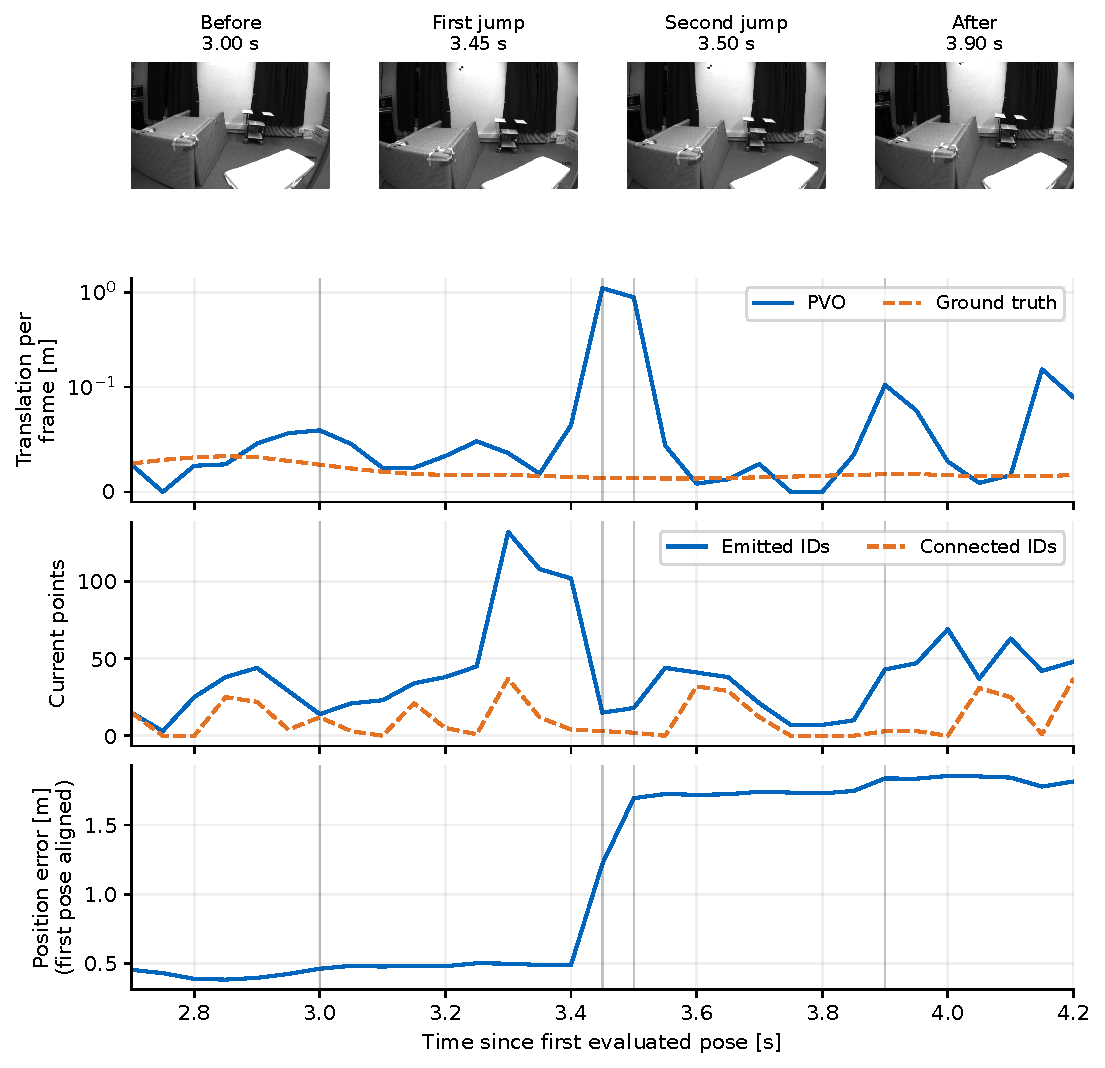
\includegraphics[width=\textwidth]{figures/evaluation/failure-ev202-early-jumps}
  \caption[Large translation estimates during small motion on EV202]{EV202's consecutive large translation estimates during small
  ground-truth motion. The native views change little across the updates, while
  only a few emitted IDs connect to existing landmarks. The position error uses
  first-pose alignment and is not globally aligned ATE.}
  \label{fig:failure-ev202-early}
\end{figure}

\begin{figure}[p]
  \centering
  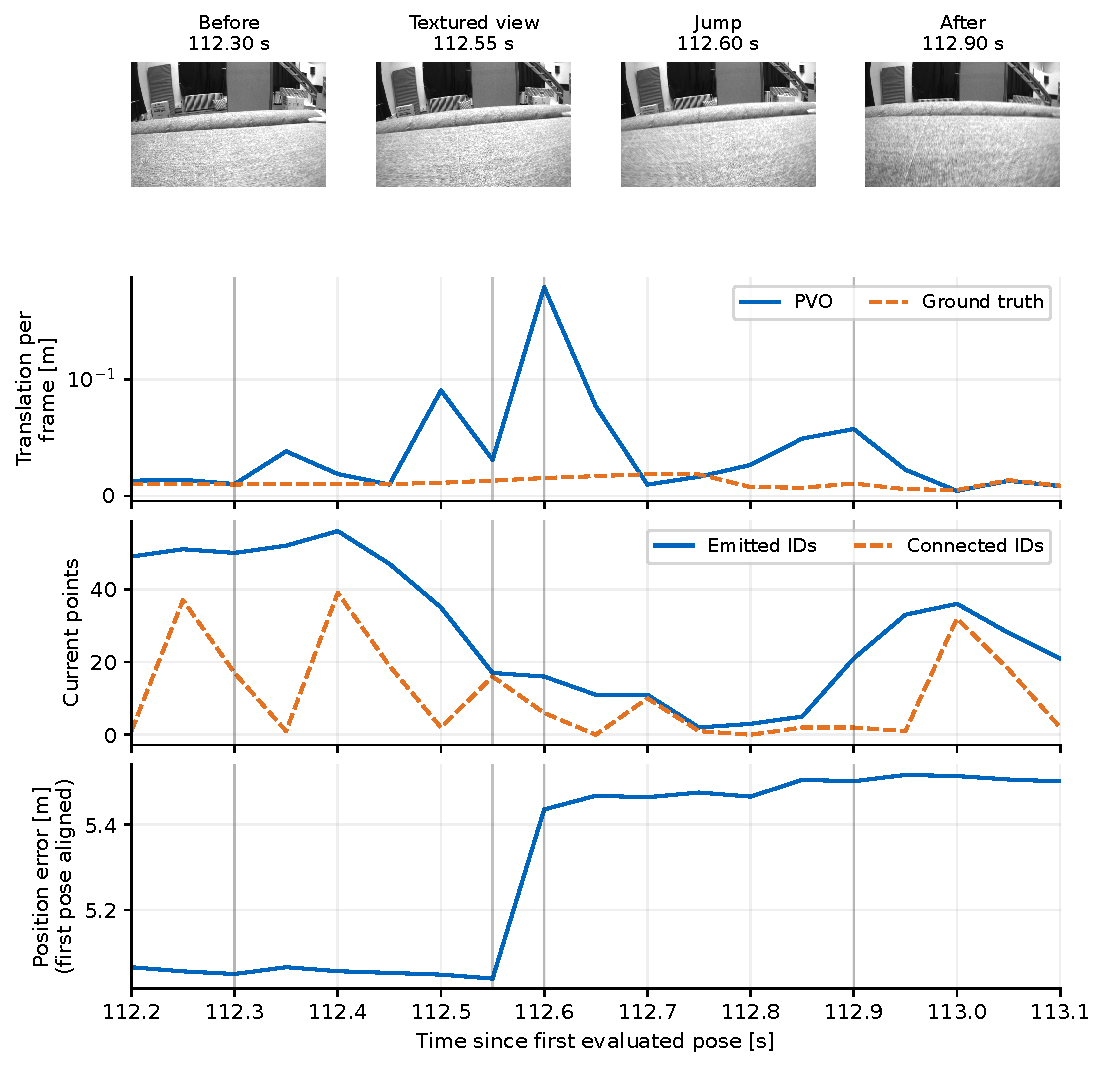
\includegraphics[width=\textwidth]{figures/evaluation/failure-ev202-textured-jump}
  \caption[EV202 failure despite abundant image texture]{An EV202 failure despite abundant visible texture. The jump frame
  contains 1640 offline Shi-Tomasi corners but only six IDs connected to existing
  landmarks. Estimated translation is \SI{0.752}{\metre}, compared with a
  ground-truth step of \SI{0.015}{\metre}. High image corner count is therefore
  not sufficient to establish usable geometric support.}
  \label{fig:failure-ev202-textured}
\end{figure}

\clearpage
\section{Full-Sequence Trajectories}\label{appendix:full-trajectories}

The following plots show PVO on all eleven EuRoC sequences, complementing the
examples in \autoref{sec:trajectory-geometry}.
Each pair of projections shows every saved PVO position after the single
whole-trajectory alignment used for ATE, together with the available reference
path. No scale correction, smoothing, or removal of failure segments is
applied. The axes use equal metric scale within a sequence and retain its full
extent. These spatial views complement, rather than replace, the timestamped
failure episodes.

EV202's estimated path is substantially distorted despite its small ATE
improvement over the stationary baseline. EMH04 retains broad excursions but
differs markedly in their geometry and vertical extent. EV103 contains a large
discontinuity far outside the reference path. Because alignment is fitted over
the complete sequence, this failure also shifts the earlier plotted estimates
relative to ground truth; their offset must not be interpreted as an initial
pose error.

\begin{figure}[p]
  \centering
  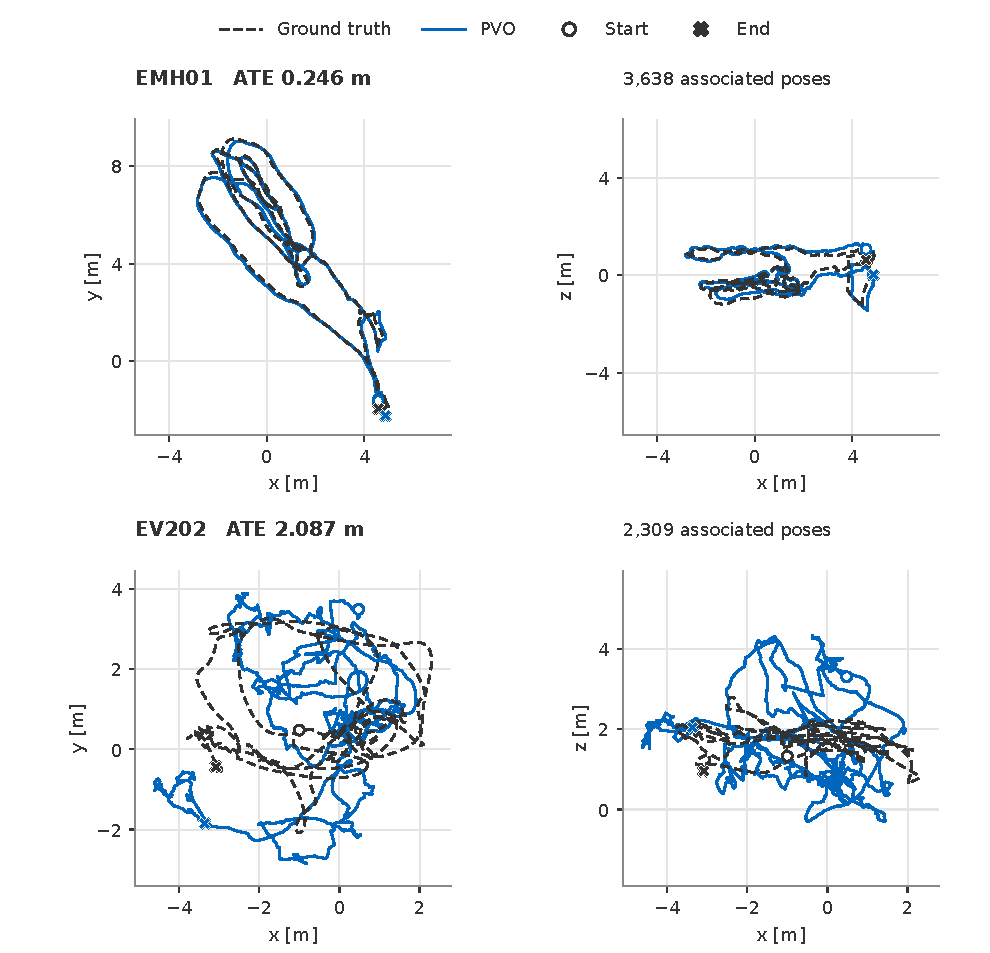
\includegraphics[width=\textwidth]{figures/evaluation/camera-trajectory-main-emh01-ev202}
  \caption[PVO trajectories on EMH01 and EV202]{Full-sequence PVO trajectories and ground truth for EMH01 and EV202,
  viewed in the $xy$ and $xz$ planes. Both views use the same rigid alignment
  as ATE, without scale correction. All saved estimates are shown; the pose
  counts identify those associated with ground truth for the reported metric.
  Circles and crosses mark the start and end of each displayed path.}
  \label{fig:trajectory-emh01-ev202}
\end{figure}

\begin{figure}[p]
  \centering
  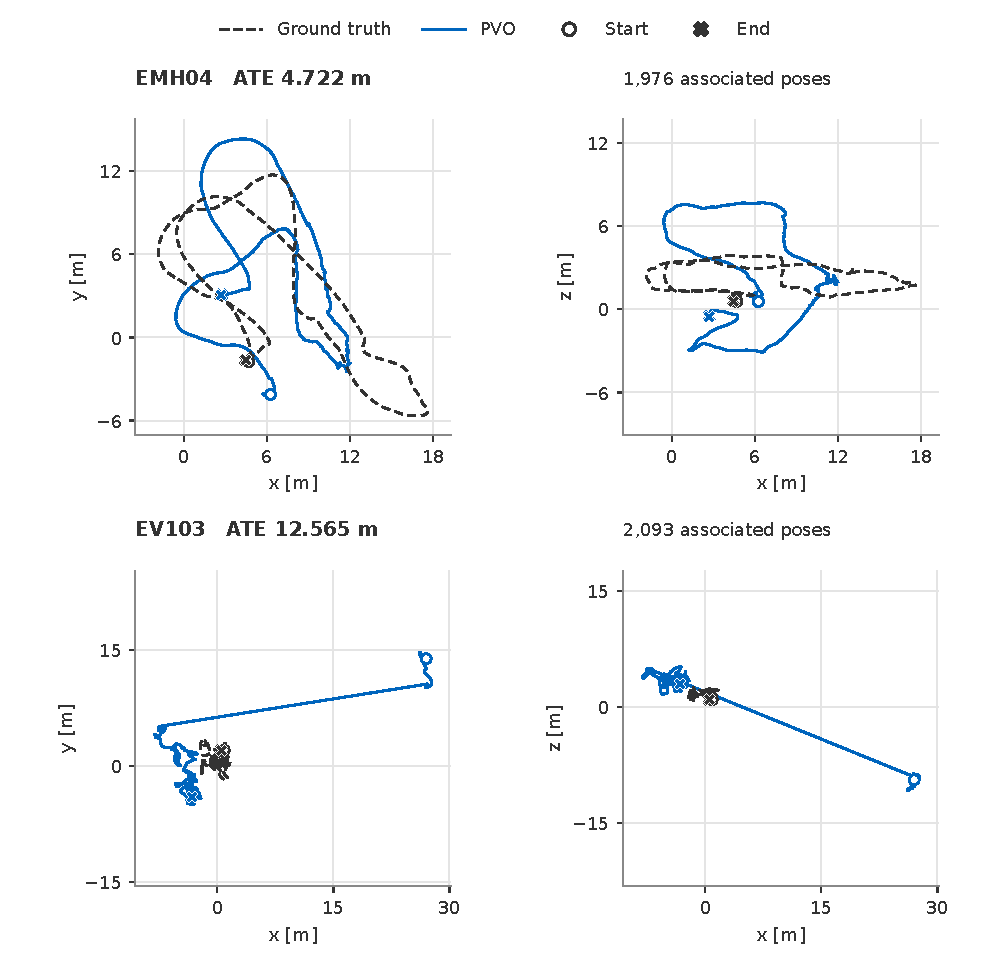
\includegraphics[width=\textwidth]{figures/evaluation/camera-trajectory-main-emh04-ev103}
  \caption[PVO trajectories on EMH04 and EV103]{Full-sequence PVO trajectories for EMH04 and EV103, using the same
  convention as \autoref{fig:trajectory-emh01-ev202}. The axes retain the full
  estimated extent, including EV103's catastrophic jump. Distances are equally
  scaled within each sequence, but axis ranges differ between sequences.}
  \label{fig:trajectory-emh04-ev103}
\end{figure}

\begin{figure}[p]
  \centering
  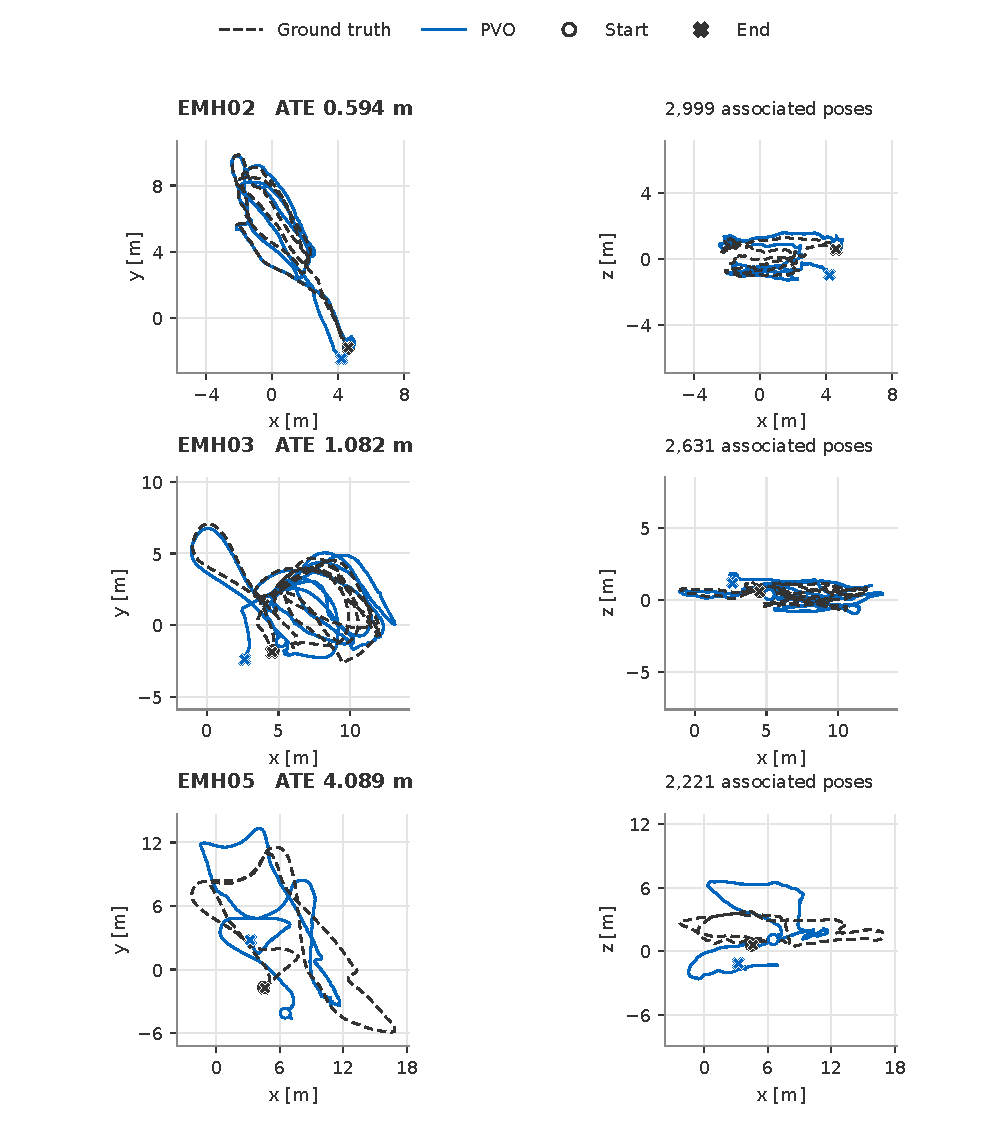
\includegraphics[width=\textwidth]{figures/evaluation/camera-trajectory-appendix-machine-hall}
  \caption[PVO trajectories on EMH02, EMH03, and EMH05]{Full-sequence PVO trajectories for the Machine Hall sequences
  EMH02, EMH03, and EMH05. Left: $xy$ projection; right: $xz$ projection.
  Circles and crosses mark the start and end of each displayed path.}
  \label{fig:trajectory-remaining-machine-hall}
\end{figure}

\begin{figure}[p]
  \centering
  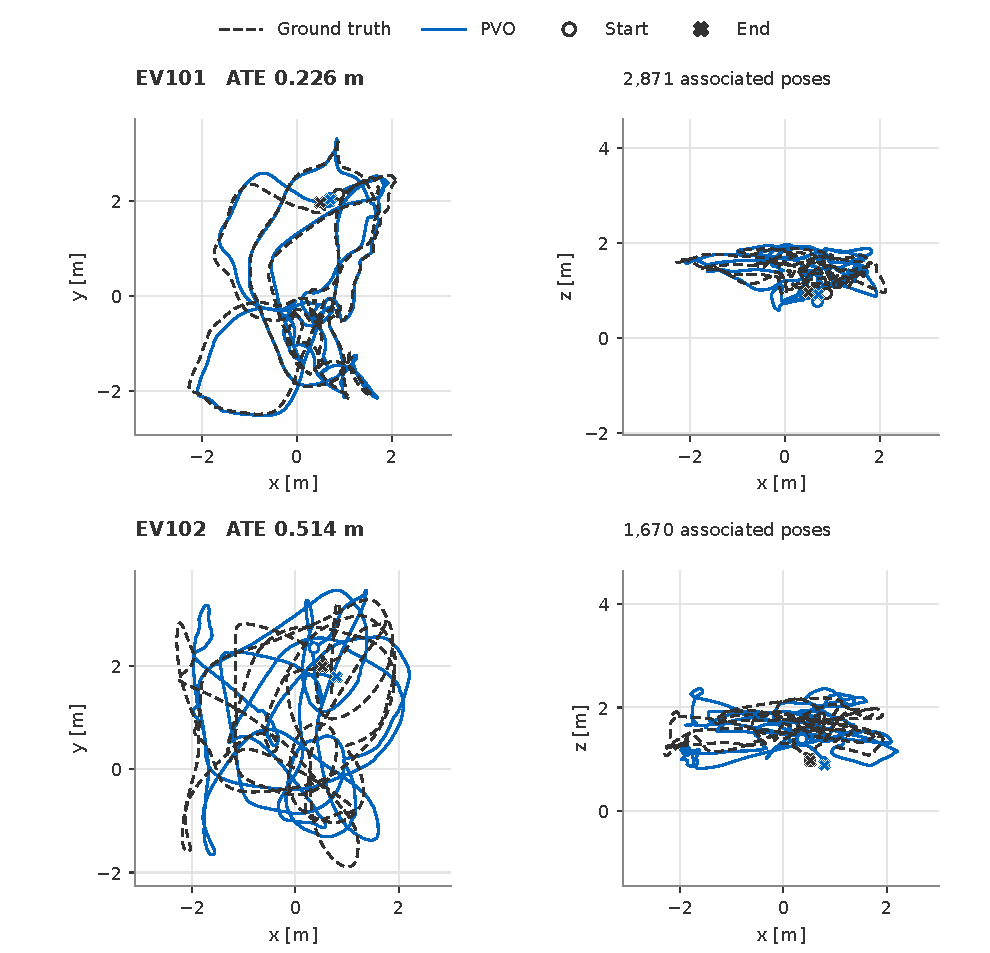
\includegraphics[width=\textwidth]{figures/evaluation/camera-trajectory-appendix-vicon-1}
  \caption[PVO trajectories on EV101 and EV102]{Full-sequence PVO trajectories for EV101 and EV102, using the same
  alignment and plotting convention as \autoref{fig:trajectory-emh01-ev202}.}
  \label{fig:trajectory-remaining-vicon-1}
\end{figure}

\begin{figure}[p]
  \centering
  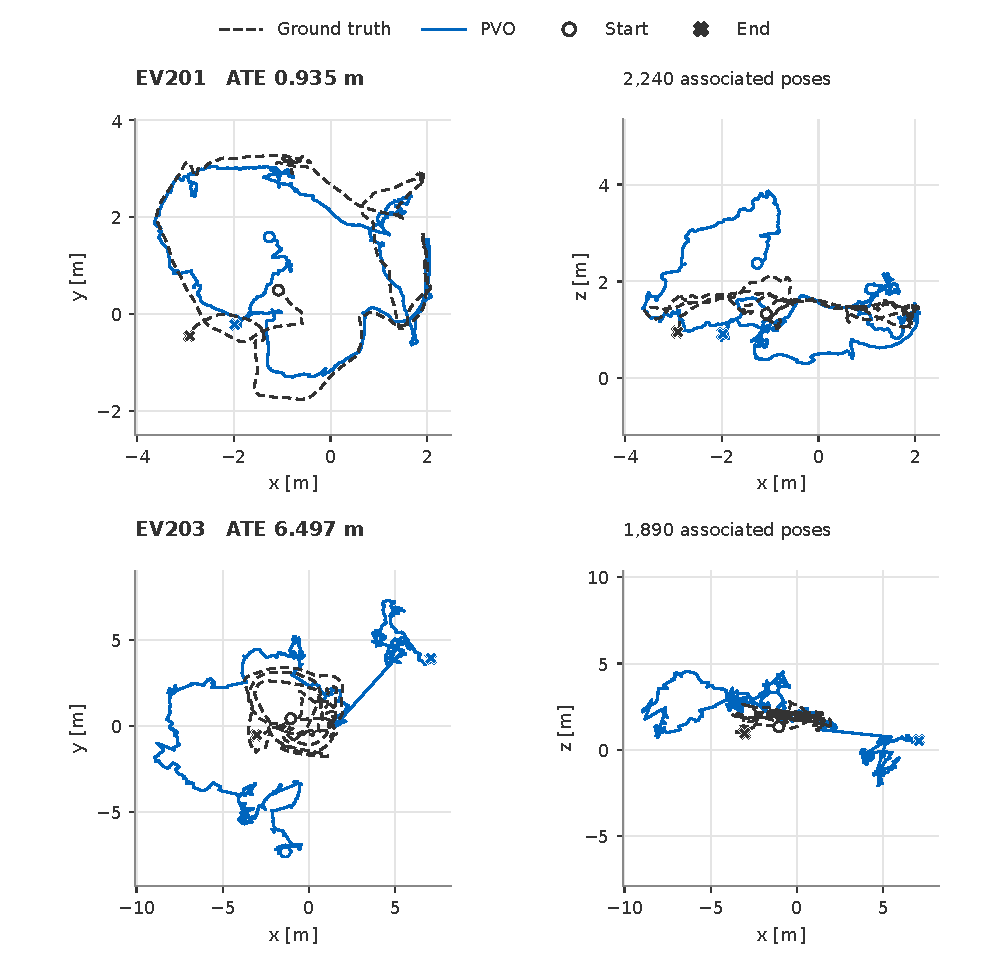
\includegraphics[width=\textwidth]{figures/evaluation/camera-trajectory-appendix-vicon-2}
  \caption[PVO trajectories on EV201 and EV203]{Full-sequence PVO trajectories for EV201 and EV203. The full extent of
  EV203's estimated motion is retained despite its much smaller reference path.}
  \label{fig:trajectory-remaining-vicon-2}
\end{figure}


\clearpage
\section{Stereo Transform Overview}\label{appendix:stereo-transforms}

The full set of twelve transformed encodings is illustrated on a later EMH02
stereo pair in \autoref{fig:stereo-all-shifts}. The rows vary disparity
pre-shift and the columns vary grid phase. This overview complements the
sampling construction and the location-specific recovery examples in
Chapter~\ref{chapter:method}.

\begin{figure}[htbp]
  \centering
  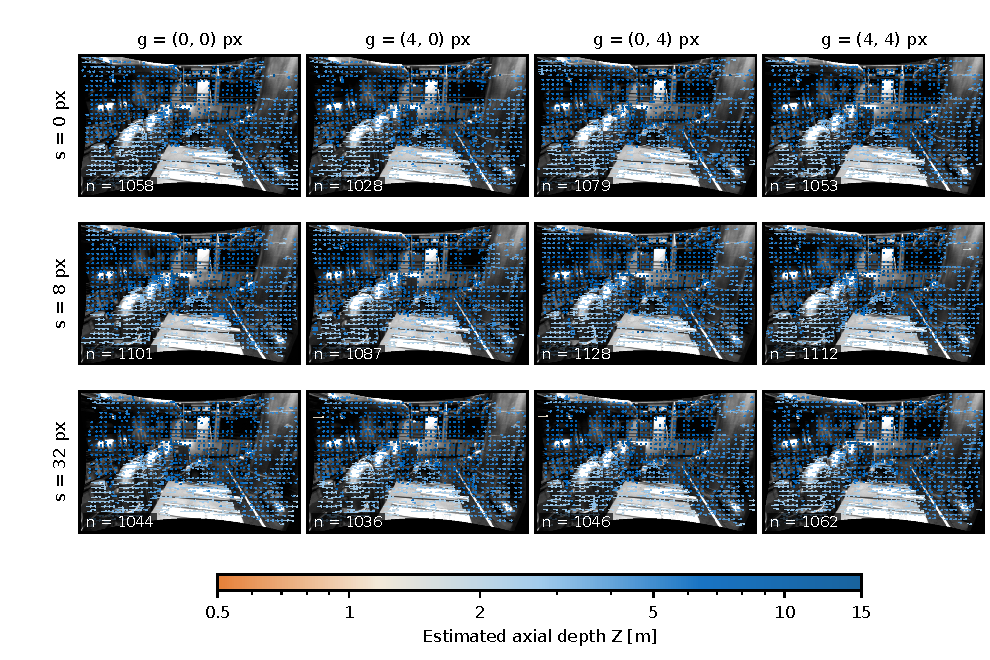
\includegraphics[width=\textwidth]{figures/method/stereo-all-shifts-late-emh02.pdf}
  \caption[Stereo correspondences across all twelve shifts]{All twelve stereo transforms for EMH02 at \SI{135}{\second}
  (pair 2700, zero based). Rows vary pre-shift $s$ and columns vary common
  grid phase $g$. Dots mark left-image locations; segments end at their
  right-image coordinates in the common rectified plane. Every
  positive-disparity observation surviving the diagnostic stereo checks is
  shown, with count $n$. Colour encodes estimated axial depth, clipped to
  the displayed \SIrange{0.5}{15}{\metre} scale.}
  \label{fig:stereo-all-shifts}
\end{figure}

% !TeX root = ../main.tex

\clearpage
\section{Lessons from Preliminary Experiments}\label{appendix:prior-experiments}

Several approaches preceded the stereo-depth alignment method developed in
this thesis. They explored filtering codec motion, using it to propagate
existing image features, and changing the lifetime or placement of tracked
samples. The examples below come from archived development experiments on
Monado sequences~\cite{deMayoCremersPireMSD}. Some used image features, inertial
rotation, or ground-truth geometry to investigate particular limitations; they
are separate from the final pixel-free EuRoC evaluation. Their common lesson
is that useful local motion and persistent point identity are distinct
requirements.

\subsection{Frequency-Based Selection of Motion Vectors}

An early idea was to distinguish coherent camera-induced motion from irregular
codec predictions through their frequency content. Motion-vector fields were
sampled on an eight-pixel grid and decomposed into spatial or spatiotemporal
frequency bands. A complementary temporal diagnostic compared successive
fields after alignment using the coded displacements. For two aligned motion
samples $\mathbf{m}_a$ and $\mathbf{m}_b$, the normalized two-point Fourier
transform has coefficients
\begin{equation}
  \frac{\mathbf{m}_a+\mathbf{m}_b}{2}
  \quad\text{and}\quad
  \frac{\mathbf{m}_a-\mathbf{m}_b}{2}.
\end{equation}
The second coefficient measures disagreement between the samples. A small
value suggests temporal consistency, but can also occur when both samples
share an incorrect displacement. A three-dimensional FFT over the two-frame
volume additionally measures spatial variation.

The diagnostic assigned each vector to the frequency band with the largest
reconstructed magnitude, provided that band's share of the summed magnitudes
exceeded a chosen dominance threshold. Spatial and spatiotemporal bands used
normalized radial cuts of 0.12 and 0.35.

\begin{figure}[!htbp]
  \centering
  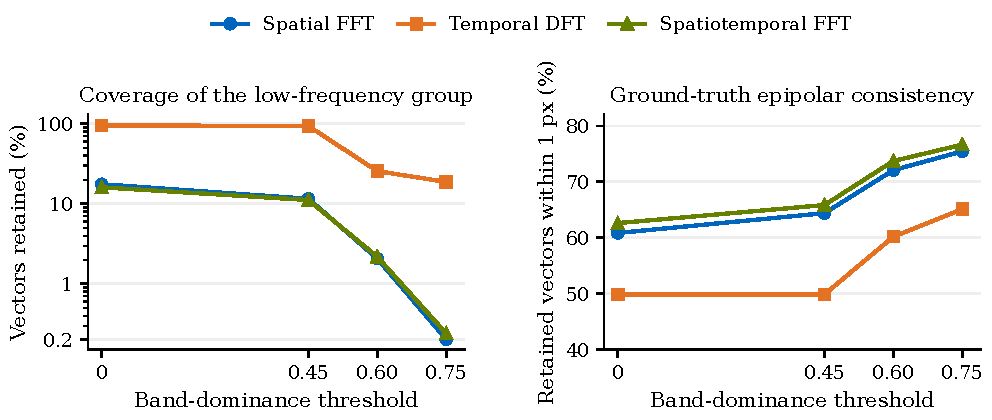
\includegraphics[width=\textwidth]{figures/appendix/prior-fft-coverage-consistency}
  \caption[Frequency selection: coverage and epipolar consistency]{Low-frequency
  selection on MOO06. Coverage uses a logarithmic axis. Consistency measures
  the fraction of retained vectors with ground-truth square-root Sampson
  residual at most one pixel, evaluated in undistorted coordinates and scaled
  by $\sqrt{f_xf_y}$. Spatial grouping covers 7,108,462 vectors; the temporally
  aligned methods cover 7,017,517 because they require a preceding field.}
  \label{fig:prior-fft-selection}
\end{figure}

\autoref{fig:prior-fft-selection} shows the resulting trade-off on MOO06.
At a threshold of 0.45, the spatiotemporal low-frequency group retained
11.15\% of the input vectors; 65.85\% of those satisfied the one-pixel
ground-truth epipolar check. Raising the threshold to 0.75 increased that
fraction to 76.65\%, but retained only 0.24\% of the vectors. Frequency
selection could therefore enrich a geometrically consistent subset at a
substantial cost in coverage. Even a small epipolar residual does not
establish the correct endpoint along the epipolar line or the identity of a
physical scene point.

A later variant ranked blocks by the sum of their reconstructed band
magnitudes and selected up to ten translation-support correspondences from
low-ranked blocks containing active features, for an inertial-rotation-assisted
epipolar filter. This score was called ``energy'' during development, although
it was not squared Fourier energy. Without image refinement of these
supports, global ranking produced \SI{0.538}{\metre} ATE RMSE on the full
4,171-frame MOO06 run, compared with
\SI{0.177}{\metre} for image-refined translation support. Selecting supports
within spatial windows improved the ranked variant to
\SI{0.299}{\metre}. These run-level results evaluate support sets, not the pose
consistency of the single lowest-scoring vector; they therefore do not settle
the latter question.

\subsection{Propagating Existing Features}

Another approach retained the identities of existing image features and
propagated their coordinates with codec displacements. At each transition,
it selected a motion vector whose source support contained the current
feature location, applied that vector, and stored the endpoint under the
same track ID. The attraction was to reuse an established feature-based
backend while replacing repeated temporal image matching. However, carrying
an ID forward does not verify that its new coordinate still observes the
same physical point.

\autoref{fig:prior-mv-propagation} illustrates the difference between a
promising short run and sustained tracking on MIO07. The archived direct-MV
prototype reached approximately \SI{0.096}{\metre} ATE over its first 800
frames, but approximately \SI{30.27}{\metre} over the full 4,095-frame
sequence. The image-based reference finished at approximately
\SI{0.120}{\metre}. The prototype still assigned vectors to 92.8\% of
attempted feature propagations. That count describes available assignments,
not their geometric correctness or preservation of point identity.

\begin{figure}[htbp]
  \centering
  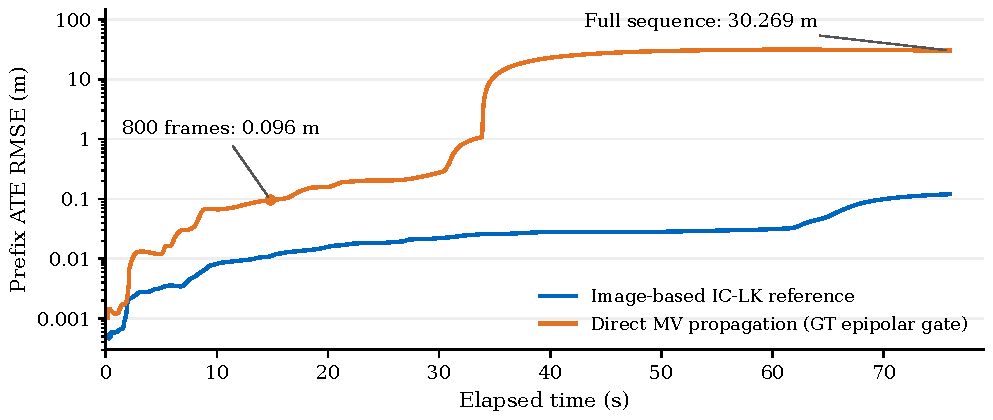
\includegraphics[width=\textwidth]{figures/appendix/prior-mv-propagation-prefix-error}
  \caption[An early direct-MV propagation failure]{Archived MIO07 development
  run: direct temporal MV propagation and an image-based inverse-compositional
  Lucas--Kanade reference. Each plotted ATE is evaluated over the prefix ending
  at that time, with a new rigid alignment and fixed scale for that prefix.
  The vertical axis is logarithmic. The direct-MV prototype used a
  ground-truth epipolar gate with a loose 32-pixel threshold, retaining
  99.6\% of input vectors; it was not an oracle for correct point identity.
  Image-based feature detection and stereo matching were retained; codec
  vectors replaced temporal tracking only.
  The curves are redrawn from the archived per-prefix measurements and do not
  represent the final PVO configuration.}
  \label{fig:prior-mv-propagation}
\end{figure}

This failure does not isolate identity drift as its sole cause: geometric
support, stereo observations, and backend conditioning also matter. It shows
why short-prefix accuracy and high assignment counts were insufficient
validation. The feature-seeded diagnostic in
\autoref{fig:mv-feature-departure-example} shows a local mechanism: codec
propagation can depart from an image track despite a common starting point
and continuing vector support.

\FloatBarrier
Further tests examined feature placement and temporal connectivity
separately. In a stereo-inertial test with spatial refill opportunities
controlled, using arbitrary codec block centres as starting locations
reduced successful temporal KLT
counts to 35.8\% of the FAST-location reference on MIO07 and 37.1\% on
MOO07. This experiment retained image-based tracking and did not use codec
displacements; it showed that block centres were not interchangeable with
selected image features. In a separate visual-only stereo test on 800 MIO07 frames using KLT
correspondences, restricting landmarks to adjacent frame pairs produced
\SI{0.521}{\metre} ATE. Making every frame a keyframe improved this to
\SI{0.035}{\metre}, while persistent tracks achieved
\SI{0.011}{\metre}. Shorter identities therefore also required changes to
landmark admission and map connectivity; they were not a complete solution
on their own.

\subsection{Persistent Surfaces with Changing Point Support}

These observations suggest a direction beyond improving a point-selection
rule. The useful codec support on an extended surface can change from frame
to frame. For example, observations on a tabletop might shift between its
edge, a corner, and an interior textured region. Such observations may remain
compatible with the motion of the same static surface even when they cannot
be joined into one long-lived point track. This is a motivation for testing
surface-level association, not evidence that the present experiments already
recover object identities.

Li and Song~\cite{li2014toward} provide a relevant precedent under a planar
scene model. They group codec correspondences using homography RANSAC,
associate planes across frames, and jointly estimate plane geometry and
camera motion in an extended Kalman filter. Their state can retain a plane
while its supporting point correspondences change. The observation model
still uses those correspondences through a plane-induced homography; the
plane label alone does not supply camera motion.

A future codec-based estimator could similarly maintain a static plane or
other geometric region while renewing its short-lived correspondence support.
It would need reliable region association, enough spatially distributed
observations, and geometry that constrains the camera motion. Merely seeing
another part of the same object would not satisfy these requirements.
Non-planar objects would require an appropriate shape or rigid-body model,
and independently moving objects would need separate treatment. Preserving
the pixel-free boundary would also require forming and associating these
regions from codec metadata and geometry. The stereo-depth construction in
this thesis supplies one possible source of that geometry; whether a surface
representation makes better use of intermittent codec support remains an
open experimental question.



\microtypesetup{protrusion=false}
\listoffigures{}
\listoftables{}
\microtypesetup{protrusion=true}
\printglossaries
\printbibliography{}

\end{document}
